%  LaTeX support: latex@mdpi.com
%  MDPI MAKE submission — main_paper_MAKE30.tex
%  English version of main_paper_NN30.tex (Japanese draft, version 30)
%  Compiled with official mdpi.cls
%  Compile: pdflatex main_paper_MAKE30.tex
%           pdflatex main_paper_MAKE30.tex
%           pdflatex main_paper_MAKE30.tex

%=================================================================
\documentclass[make,article,submit,pdftex,moreauthors]{Definitions/mdpi}

%=================================================================
% MDPI internal commands — do not modify
\firstpage{1}
\makeatletter
\setcounter{page}{\@firstpage}
\makeatother
\pubvolume{8}
\issuenum{1}
\articlenumber{0}
\pubyear{2026}
\copyrightyear{2026}
%\externaleditor{Firstname Lastname}
\datereceived{ }
\daterevised{ }
\dateaccepted{ }
\datepublished{ }

%=================================================================
% Notation shorthands (kept in sync with main_paper_NN30.tex)
\newcommand{\dID}{d_{\mathrm{ID}}}
\newcommand{\dz}{m}
\newcommand{\dzopt}{m^{\mathrm{cand}}}
\newcommand{\dtrue}{d_{\mathrm{true}}}
\newcommand{\Jg}{J_g}
\newcommand{\R}{\mathbb{R}}
\newcommand{\kap}{\kappa}
\newcommand{\AUsat}{\mathrm{AU}_{\mathrm{sat}}}
\newcommand{\dzsat}{m^{\mathrm{sat}}}
\newcommand{\mknee}{m^{\mathrm{knee}}}
\newcommand{\demb}{d_{\mathrm{emb}}}
\newcommand{\hatdID}{\hat{d}_{\mathrm{ID}}}

%=================================================================
\Title{Diagnostic Interpretation of Effective Latent Dimensionality in
Autoencoders and Variational Autoencoders}

% ORCID IDs (replace 000X with actual ORCID or comment out)
%\newcommand{\orcidauthorA}{0000-0000-0000-000X}
%\newcommand{\orcidauthorB}{0000-0000-0000-000X}
%\newcommand{\orcidauthorC}{0000-0000-0000-000X}

\Author{Chika Obata $^{1}$,
        Mizuki Dai $^{1}$, and
        Kenya Jin'no $^{1,}$*}

\AuthorNames{Chika Obata, Mizuki Dai, and Kenya Jin'no}

\address{%
$^{1}$ \quad Department of Intelligent Systems,
  Faculty of Information Engineering,
  Tokyo City University,
  1-28-1 Tamazutsumi, Setagaya-ku, Tokyo 158-8557, Japan;
  g2332016@tcu.ac.jp (C.O.); g2591402@tcu.ac.jp (M.D.)}

\corres{Correspondence: kjinno@tcu.ac.jp; Tel.: +81-3-5707-0104 (K.J.)}

%=================================================================
\abstract{%
This paper proposes a multi-indicator diagnostic framework that integrates
active-unit (AU) dynamics, intrinsic-dimension (ID) estimation (TwoNN/MLE),
reconstruction-error (MSE) elbows, and PCA baselines to diagnostically
interpret the effective latent dimensionality actually used in the
representations learned by autoencoders (AEs) and variational autoencoders
(VAEs).
The goal of the framework is not to determine the effective latent
dimensionality as a single unique number.
Rather, it explicitly separates the diagnostic roles of the indicators:
AU values serve as direct observations of the number of latent coordinates a
VAE actually uses; TwoNN/MLE ID estimates serve as numerically stable
auxiliary reference estimators; and the AU slowdown point $\mknee$ is treated
as an exploratory change point subject to grid and seed dependence.
Effective-dimension usage is then diagnosed from the consistency of the
multiple indicators.
Theoretically, under a rate--distortion surrogate of the linear-Gaussian
$\beta$-VAE, we derive the condition $\lambda_j > \beta\tau^2$ for the $j$-th
eigendirection of the data covariance to be activated, explaining the
mechanism by which KL regularization suppresses effective latent
dimensionality from a water-filling perspective.
This analysis is positioned not as a rigorous theorem for nonlinear VAEs but
as a linear surrogate model for interpreting the experimental results.
Experimentally, we show that in fully connected VAEs trained on MNIST, AU
values and TwoNN IDs are highly reproducible across random seeds, whereas
$\mknee$ fluctuates strongly on sparse $m$-grids.
By densely searching the neighborhood of the estimated ID and evaluating with
independently initialized multi-seed runs, $\mknee$ stabilizes at
$10.3 \pm 0.9$, consistent with the TwoNN ID near 10.
Furthermore, through Fashion-MNIST, Conv-VAE, and CIFAR-10/SVHN experiments,
we quantify the conditions under which the proposed diagnostic framework
functions effectively and the boundary conditions under which AU/$\mknee$
diagnostics become inconclusive.}

\keyword{variational autoencoder; effective latent dimensionality;
active units; intrinsic dimension; TwoNN; diagnostic framework;
representation learning; knowledge extraction; posterior collapse}

%=================================================================
\begin{document}

\section{Introduction}\label{sec:intro}

\subsection{Background: The Problem of Interpreting Effective Latent Dimensionality}\label{sec:intro_bg}

In representation learning, autoencoders (AEs) and
variational autoencoders (VAEs)~\cite{kingma2014vae} are
core unsupervised models that learn low-dimensional latent representations
from high-dimensional data~\cite{bengio2013representation}.
The most fundamental design parameter governing the ``quality'' of these
latent representations is the bottleneck dimension~$m$:
if $m$ is too small, information is lost, whereas if it is too large,
redundant dimensions arise (and, in VAEs, posterior collapse~\cite{lucas2019elbo} worsens).

However, a methodology for quantitatively reading ``how many dimensions a
learned latent representation actually uses''---that is, the
\textbf{effective latent dimensionality}---has not been sufficiently
established in deep representation learning research.
Existing studies~\cite{ansuini2019intrinsic,valeriani2023geometry} have
measured the intrinsic dimension of individual layers of deep networks,
but studies that systematically analyze the effective dimensionality at the
bottleneck of AEs/VAEs together with its training dynamics remain limited.

The central question addressed in this paper is:
\begin{quote}
\textit{How do AEs/VAEs ``learn'' the local intrinsic dimensionality and the
topological embedding dimensionality of the input data as the effective
dimensionality of the latent space?
And is there a way to quantitatively read this effective dimensionality
from the outside?}
\end{quote}

\subsection{Positioning and Contributions of This Study}\label{sec:intro_aim}

To address this question, we propose a
\textbf{multi-indicator diagnostic framework} built on two pillars:
\textbf{intrinsic-dimension (ID) estimation} and \textbf{active-unit (AU) dynamics}.
The novelty of the framework lies not in ``uniquely determining'' the
effective dimensionality with a single indicator, but in combining the
indicators while making the robustness and exploratory character of each
explicit, and \textbf{interpreting them diagnostically}.
We do not claim that ``$\mknee$ uniquely identifies an appropriate
bottleneck dimension''---$\mknee$ is a coarse exploratory design guide,
and the primary readout of effective dimensionality is carried by the
robust indicator (AU values) and the numerically stable auxiliary
reference estimator (TwoNN ID).

\textbf{Roles and robustness of each indicator}:
\begin{itemize}
  \item \textbf{TwoNN/MLE ID}: numerically stable auxiliary reference
        estimators that infer the effective degrees of freedom from local distances
        (across-seed $\sigma \leq 0.12$; subject to isometry bias; Section~\ref{sec:exp_multiseed2}).
  \item \textbf{AU values}: a robust indicator that directly observes whether the
        KL-regularized VAE actually uses each dimension
        (across-seed $\sigma \leq 0.5$; independent of the distance preservation of the
        reference AE; dependent on $\beta$, $\delta$, and model capacity).
  \item \textbf{MSE elbow and PCA}: auxiliary readouts of effective
        dimensionality from the reconstruction-error side.
  \item \textbf{AU slowdown point $\mknee$}: an exploratory indicator derived
        from the shape of the AU curve above---it coarsely captures the turning
        point at which KL regularization begins compressing dimensions,
        but its value depends on the $m$~grid and the random seed (Section~\ref{sec:exp_multiseed2}).
\end{itemize}

The \textbf{contributions of this paper are threefold}:
\begin{enumerate}
  \item \textbf{Proposal of a multi-indicator diagnostic framework}:
        The main contribution of this study is not the proposal of $\mknee$ itself,
        but the organization of AU values, TwoNN/MLE ID, the MSE elbow, and PCA as
        diagnostic indicators with distinct roles, providing a framework for
        interpreting the effective latent dimensionality of AEs/VAEs from multiple
        perspectives.
        We clearly distinguish AU values as a robust indicator that directly
        observes latent-dimension usage,
        TwoNN ID as a numerically stable auxiliary reference estimator, and
        $\mknee$ as an exploratory change point obtained from the shape of the AU curve
        (Sections~\ref{sec:framework} and~\ref{sec:discussion}).
        Three-seed verification on MNIST confirms the high reproducibility of
        AU values ($\sigma \leq 0.5$) and TwoNN ID ($10.03 \pm 0.12$), and we
        present $\mknee = 10.3 \pm 0.9$ under dense-grid, independent-initialization,
        multi-seed conditions (Exp-Mnist-Dense-300) as the main stabilization result
        (Section~\ref{sec:exp_el}).
  \item \textbf{Derivation of the AU activation condition based on a linear-Gaussian
        rate--distortion surrogate}:
        Under the linear-Gaussian $\beta$-VAE rate--distortion surrogate, we derive
        the condition $\lambda_j > \beta\tau^2$ for the $j$-th latent dimension to be
        active, using the water-filling theorem and the KKT conditions
        (Theorem~\ref{thm:linear_vae}, Section~\ref{sec:theory}), and explain the
        mechanism by which KL regularization suppresses effective dimensionality
        from the perspective of the water-filling principle.
        This result is not a rigorous theorem for actual non-linear VAEs; it is an
        analytical result based on the linear-Gaussian rate--distortion surrogate
        that provides a qualitative correspondence with the non-linear experiments.
  \item \textbf{Quantification of the applicability range and limiting conditions}:
        Targeting MNIST/Fashion-MNIST (FC-VAE), Conv-VAE, and CIFAR-10/SVHN, we
        empirically demonstrate the reproducibility of AU values and TwoNN ID,
        the grid and seed dependence of $\mknee$, and that
        ``$m \gg \hat{d}_\mathrm{ID}$ is the dominant condition for TwoNN stability,
        more important than isometry improvement''
        (Exp-Real-Geom, Proposition~\ref{thm:twonn_stability}).
        Furthermore, for Conv-VAEs and natural images, we quantify the boundary
        conditions under which AU/$\mknee$ diagnostics become difficult, as five
        operational criteria for stable identification
        (Sections~\ref{sec:disc_convvae} and~\ref{sec:disc_limitation}).
\end{enumerate}

\subsection{Two Kinds of ``Dimension'': Local Intrinsic Dimension and Topological Embedding Dimension}\label{sec:intro_dim}

In this paper, we distinguish two notions of manifold ``dimension'':
$\dID$ (the local intrinsic dimension, the target of TwoNN/MLE estimation) and
$\demb$ (the topological minimal embedding dimension, the minimal dimension
required for an embedding without self-intersection)
(for the Swiss Roll, $\demb = \dID = 2$; for the Torus, $\demb = 3 > \dID = 2$).

Note, however, that \textbf{the main contribution of this paper is not to prove a
correspondence with $\dID$ or $\demb$, but to organize the robustness, limits,
and applicability conditions of the diagnostic indicators AU values, TwoNN ID,
and $\mknee$}.
The conditional correspondence between $\demb$ and $\AUsat$ (for the Torus,
M\"obius strip, etc.) is positioned as an incidental supporting observation
(Section~\ref{sec:disc_incidental}).

\subsection{Research Questions}\label{sec:intro_rq}

\begin{description}
  \item[RQ1] Under what grid-density, seed-count, and architecture conditions can
             the change point $\mknee$ obtained from the AU dynamics of a VAE be
             used as a diagnostic auxiliary quantity consistent with TwoNN/MLE
             ID estimates?
  \item[RQ2] Does a framework that interprets the effective latent dimensionality
             of AEs/VAEs with multiple indicators (AU values, TwoNN/MLE, the MSE
             elbow, and PCA) provide complementary information relative to any
             single indicator?
  \item[RQ3] How do bottleneck headroom (the magnitude of $m / \hat{d}_\mathrm{ID}$)
             and geometric regularization (IsometricAE) affect the stability of
             TwoNN ID estimation?
\end{description}

\subsection{Paper Organization}\label{sec:intro_structure}

\textbf{Explicit scope of validation}:
The validation in this paper covers synthetic manifolds
($d_{\mathrm{true}} \leq 3$), MNIST and Fashion-MNIST (fully connected AE/VAE),
Conv-AE/VAE (experiments Exp-Conv-AE and Exp-Conv-Fix), KL annealing
(experiment Exp-Conv-Ann),
and natural images (CIFAR-10 and SVHN; experiments Exp-Nat-Cifar and Exp-Nat-SVHN).
In the natural-image experiments (Exp-Nat-Cifar and Exp-Nat-SVHN), we confirm
that the TwoNN auxiliary estimate yields values consistent with those reported
by Pope et al.~\cite{pope2021intrinsic}, and we further quantify the validity
range and limiting conditions of AU/$\mknee$ diagnostics for Conv-VAEs
(we do not claim ``generalization'' of the entire framework to natural images).

The paper is organized as follows:
Section~\ref{sec:related} (related work), Section~\ref{sec:framework} (framework),
Section~\ref{sec:theory} (theoretical background, including Theorem~\ref{thm:linear_vae}),
Section~\ref{sec:exp} (experiments), Section~\ref{sec:discussion} (discussion),
and Section~\ref{sec:conclusion} (conclusions).
Detailed proofs and sensitivity analyses are collected in the appendices.

%% ===================================================================
\section{Related Work}\label{sec:related}

\subsection{Representation Learning and Autoencoders}\label{sec:related_ae}

Bengio et al.~\cite{bengio2013representation} organized the theoretical
framework of representation learning and discussed the mechanism by which AEs
learn the low-dimensional structure of high-dimensional data based on the
manifold hypothesis~\cite{fefferman2016manifold}.
$\beta$-VAE~\cite{higgins2017betavae} promotes disentangled representations by
increasing the KL-regularization weight $\beta$, which directly affects AU.
Lucas et al.~\cite{lucas2019elbo} analyzed, within a linear-VAE framework, the
conditions under which posterior collapse (a substantial reduction of AU)
occurs in ELBO minimization, and showed theoretically that AU saturates near
$d_{\mathrm{ID}}$.
From the perspective of score matching, the DAE analysis~\cite{alain2014dae}
showed that the reconstruction directions of denoising autoencoders selectively
suppress the normal directions of the manifold.
The CAE~\cite{rifai2011cae} learns contractive representations by regularizing
the encoder-side Jacobian.

\subsection{Intrinsic-Dimension Analysis of Deep Representations}\label{sec:related_id}

Pope et al.~\cite{pope2021intrinsic} showed via TwoNN estimation that the
intrinsic dimension of natural images is far lower than the pixel dimension
(CIFAR-10: $d_\mathrm{ID} \approx 26$ at $32 \times 32$).
Ansuini et al.~\cite{ansuini2019intrinsic} quantified the patterns by which ID
changes across the layers of deep networks, documenting contraction and
expansion phenomena of the representations.
Valeriani et al.~\cite{valeriani2023geometry} systematically analyzed the
geometric structure of the hidden representations of large transformer models.
Birdal et al.~\cite{birdal2021intrinsic} analyzed the relationship to
generalization error by integrating persistent homology with ID.
Our study is complementary to these works that ``measure the ID of existing
networks,'' and differs in that it tracks the formation of effective
dimensionality at the \textbf{design stage} and during the
\textbf{training dynamics} of AEs/VAEs.

As intrinsic-dimension estimation methods, we adopt
TwoNN~\cite{facco2017twonn} (two-nearest-neighbor distance ratios) and
MLE~\cite{levina2005mle} (maximum-likelihood estimation).
DANCo~\cite{ceruti2014danco} is more precise but computationally more expensive.
While UMAP~\cite{mcinnes2018umap} is widely used as a non-linear
dimensionality-reduction technique for visualization, our study focuses not on
visualization but on the \textbf{quantitative interpretation} of the bottleneck
dimension.

\subsection{Active Units and Posterior Collapse}\label{sec:related_au}

The active-unit (AU) count~\cite{lucas2019elbo,higgins2017betavae} is the
number of latent dimensions whose posterior-mean variance exceeds a threshold
$\delta$, and it quantifies the number of dimensions in which KL regularization
is functioning effectively.
Lucas et al.~\cite{lucas2019elbo} showed, within a linear-VAE framework, that
ELBO minimization induces posterior collapse and that AU saturates near
$d_{\mathrm{ID}}$.
In contrast, our Theorem~\ref{thm:linear_vae} \textbf{quantifies Lucas et al.'s
qualitative argument as the closed-form threshold $\lambda_j > \beta\tau^2$}
in terms of the data eigenvalues $\lambda_j$, the noise $\tau^2$, and the
regularization $\beta$; its novelty lies in carrying out a quantitative
derivation under the linear-Gaussian rate--distortion surrogate, using an
explicit connection to Shannon's water-filling theorem and the KKT conditions
(it also subsumes the $\beta=1$ special case of PPCA by Tipping \&
Bishop~\cite{tippingbishop1999ppca}).
Moreover, the systematic analysis of AU growth dynamics on real data---in
particular the concept of $\mknee$ and its correspondence with effective
representational dimensionality, its limiting conditions, and stabilization
strategies---is systematically validated in this study
(Theorem~\ref{thm:linear_vae}, Proposition~\ref{thm:mknee_instab},
Section~\ref{sec:disc_mknee_improve}).

\subsection{Geometric Autoencoders}\label{sec:related_geo}

Nazari et al.~\cite{nazari2023geometric} proposed geometric autoencoders,
introducing a regularizer that makes the encoder preserve the geometric
structure of the manifold.
Kato et al.~\cite{kato2020rdae} proposed IsometricAE, which realizes an
isometric embedding by driving the pullback metric of the decoder Jacobian
toward the identity matrix.
In this study, we position IsometricAE as ``an auxiliary tool that improves a
precondition (isometry) for the readout accuracy of effective dimensionality''
(RQ3, experiment Exp-Syn-Iso).

%% ===================================================================
\section{Framework: Reading Out the Effective Latent Dimensionality}\label{sec:framework}

\subsection{Problem Setup and Main Notation}\label{sec:framework_setup}

We define an AE/VAE with input dimension $N$ and bottleneck dimension $m$:
an encoder $f: \R^N \to \R^m$ and a decoder $g: \R^m \to \R^N$.
For a VAE, the encoder outputs a posterior
$q_\phi(z|x) = \mathcal{N}(\mu(x), \sigma^2(x))$,
and the KL regularization (with strength $\beta$) acts as an information bottleneck.

\textbf{Definition of Active Units (AU)}:
\begin{equation}
  \mathrm{AU}(m) = \sum_{k=1}^{m} \mathbf{1}\bigl[\mathrm{Var}_x[\mu_k(x)] > \delta\bigr],
  \quad \delta = 10^{-2}
  \label{eq:au_def}
\end{equation}
where $\mu_k(x)$ is the $k$-th component of the posterior mean and $\delta$ is a
threshold (following Lucas et al.~\cite{lucas2019elbo}).
AU is extremely robust to this threshold choice: a sensitivity analysis confirms
that the AU values remain essentially unchanged for
$\delta \in [10^{-3}, 10^{-1}]$ (see Appendix~\ref{app:delta}).

\textbf{Definition of the AU increase rate (two steps)}:
We first define the raw increase rate $s(m_i)$ on the grid as
\begin{equation}
  s(m_i) = \frac{\mathrm{AU}(m_i) - \mathrm{AU}(m_{i-1})}{m_i - m_{i-1}}
  \label{eq:au_raw_rate}
\end{equation}
where $m_{i-1}$ is the immediately preceding value on the grid.
We then define the normalized increase rate $\rho(m_i)$ as
\begin{equation}
  \rho(m_i) = \frac{s(m_i)}{\max_j s(m_j)}
  \label{eq:au_rate}
\end{equation}
so that $\rho(m_i) \in [0, 1]$.

Table~\ref{tab:notation} lists the \textbf{main notation}.

\begin{table}[H]
\begin{adjustwidth}{-\extralength}{0cm}
\centering
\caption{Notation used throughout this paper}
\label{tab:notation}
\small
\begin{tabular}{lll}
\toprule
Symbol & Meaning & Section \\
\midrule
$m$ & Bottleneck dimension (design parameter) & §\ref{sec:framework} \\
$\dzopt$ ($= m^{\mathrm{cand}}$) & Diagnostic candidate dimension (not a unique optimum) & §\ref{sec:framework} \\
$\dzsat$ ($= m^{\mathrm{sat}}$) & AU sharp saturation point (diagnostic candidate for synthetic manifolds) & §\ref{sec:framework} \\
$\mknee$ ($= m^{\mathrm{knee}}$) & AU slowdown point (rough heuristic for real data) & Equation~\eqref{eq:mknee} \\
$\AUsat$ & Maximum AU value over the grid & Equation~\eqref{eq:au_def} \\
$\hat{\dID}$ & ID estimate via TwoNN/MLE & §\ref{sec:framework} \\
$\dtrue$ & True intrinsic dimension of synthetic manifold (known) & §\ref{sec:exp_synthetic} \\
$\demb$ & Topological minimum embedding dimension ($\demb \geq \dID$) & §\ref{sec:intro_dim} \\
$\kap$ & Decoder Jacobian condition number (isometry indicator) & §\ref{sec:related_geo} \\
$s(m_i)$ & Raw AU increase rate per unit dimension & Equation~\eqref{eq:au_raw_rate} \\
$\rho(m_i)$ & Normalized AU increase rate ($\in[0,1]$) & Equation~\eqref{eq:au_rate} \\
$\tau_{\mathrm{knee}}$ & Slowdown detection threshold (default: 0.25) & Equation~\eqref{eq:mknee} \\
\bottomrule
\end{tabular}
\end{adjustwidth}
\end{table}

The core of our framework is the explicit classification of each indicator as a
\textbf{robust indicator} or an \textbf{exploratory indicator}, followed by their
complementary use (Table~\ref{tab:indicator_class}).
This classification is an empirical one grounded in the experimental findings
reported later (§\ref{sec:exp_multiseed2}), and it forms the core of a design
philosophy that systematically avoids the misdiagnoses caused by overreliance on
any single indicator.

\textbf{On the meaning of ``robust indicator'' and ``exploratory indicator''}:
``Robust'' here does not mean unbiased with respect to the true intrinsic dimension.
We use the term in the sense that, at least under our experimental conditions,
the variance with respect to random seeds is small.
``Exploratory,'' in contrast, means that the indicator is useful for grid design
and hypothesis generation but is not treated as a unique estimate of the
effective latent dimensionality.

\begin{table}[H]
\begin{adjustwidth}{-\extralength}{0cm}
\centering
\caption{Classification and empirical reliability of diagnostic indicators}
\label{tab:indicator_class}
\small
\begin{tabular}{p{3.5cm}p{3.2cm}p{4.0cm}p{4.0cm}}
\toprule
Indicator & Category & Empirical reliability (inter-seed $\sigma$) & Primary use \\
\midrule
AU values ($\mathrm{AU}(m)$) & \textbf{Robust indicator} & $\sigma \leq 0.5$ (MNIST 300ep) & Direct observation of effective dimensionality; independent of reference AE geometry (depends on $\beta$, $\delta$, model capacity) \\
TwoNN ID ($\hat{d}_\mathrm{ID}$) & \textbf{Numerically stable auxiliary reference}$^\dagger$ & $\sigma \leq 0.12$ ($m=64$) & Reference estimate of intrinsic dimension \\
MSE elbow & Auxiliary indicator & Qualitative only & Reconstruction-side verification \\
PCA cumulative variance & Auxiliary indicator & Linear assumption only & Linear baseline \\
$\mknee$ (AU slowdown point) & \textbf{Exploratory indicator} & $\sigma=15$ (sparse grid); $\sigma=0.9$ (dense grid) & Rough heuristic of effective dimensionality \\
\bottomrule
\end{tabular}
\medskip
\footnotesize
$^\dagger$ TwoNN ID is a \textbf{supplementary reference estimator} subject to isometry bias ($\kap \approx 10^9$); see §\ref{sec:framework_pipeline} for details.
$\sigma$ of $\mknee$ is for sparse grid; improved to $\sigma=0.9$ with dense grid (Exp-Mnist-Dense), where grid design is a major factor (§\ref{sec:exp_el}).
\normalsize
\end{adjustwidth}
\end{table}

\begin{Remark}[Terminology]
We distinguish the following terms throughout this paper.
The \textbf{effective latent dimensionality} is the umbrella term for the number of
bottleneck dimensions that the AE/VAE actually exploits---the quantity the
designer wishes to know.
\textbf{$\hat{d}_\mathrm{ID}$} (estimated intrinsic dimension) denotes the point estimate
obtained by TwoNN/MLE (via a reference AE, subject to isometry bias).
\textbf{$\mknee$} denotes the observational indicator of effective dimensionality
read from the AU dynamics of the VAE.
\textbf{$\AUsat$} denotes the maximum AU value over the grid (the saturation value
for synthetic manifolds; a reference value for real data).
All of these are estimates of the ``effective latent dimensionality'' obtained through
different approximation and observation procedures, and in principle they can be
expected to agree (an empirical confirmation under the conditions of this study;
§\ref{sec:exp}).
\end{Remark}

\subsection{Pipeline for Reading Out the Effective Latent Dimensionality}\label{sec:framework_pipeline}

The framework proposed in this study is an interpretation pipeline that
``reads out the effective latent dimensionality learned by an AE/VAE in two
stages'' (Figure~\ref{fig:framework}).

\textbf{Stage~1: Approximate estimation of the intrinsic dimension (auxiliary role)}

In this paper, we estimate the intrinsic dimension $\hat{d}_\mathrm{ID}$ in two ways:
(a) for \textbf{synthetic manifolds}, TwoNN/MLE is applied directly in the input
space (allowing comparison with $\dtrue$);
(b) for \textbf{real data (MNIST, etc.)}, to avoid the curse of high
dimensionality, the estimate is obtained via the latent representation of a
larger reference AE ($m_{\mathrm{ref}} = 256$).

\textbf{Explicit statement of limitations}: The latent space of the reference AE
in method (b) ($m = 256 \gg \hat{d}_\mathrm{ID}$) does not guarantee isometry
(auxiliary measurement: $\kap \approx 10^9$; §\ref{sec:disc_limitation}),
so the resulting $\hat{d}_\mathrm{ID}$ is an approximation subject to isometry bias.
In this paper, we treat $\hat{d}_\mathrm{ID}$ as \textbf{auxiliary prior information}
indicating the candidate range for $\mknee$, and by design we entrust the primary
readout of the effective dimensionality to the AU dynamics of Stage~2.
This avoids circular reasoning stemming from the non-isometry of the reference AE.
We ensure practical stability by confirming that the estimates converge across
multiple values of $m$ (e.g., $\{64, 128, 256\}$).

\textbf{Stage~2: Reading out the effective dimensionality via AU dynamics}

We sweep the bottleneck dimension $m$ over the discrete grid
$\mathcal{M} = \{1, 2, 4, 8, 12,\allowbreak 16, 20, 32,\allowbreak 64, 128, 256\}$,
training a VAE ($\beta = 4$) at each $m$ and computing $\mathrm{AU}(m)$.
Depending on the AU pattern, we read the diagnostic candidate dimension
$\dzopt$ ($= m^{\mathrm{cand}}$) in one of two ways
(\textbf{$\dzopt$ is not the unique ``optimal'' bottleneck dimension but a
diagnostic candidate dimension based on multiple indicators}):

\begin{description}
  \item[Saturation type (simple data such as synthetic manifolds)]
        When AU saturates sharply at a specific $m$, we use that saturation point
        $\dzsat$ as the diagnostic candidate dimension $\dzopt = \dzsat$
        (since AU values are robust, this is quite reliable under these
        conditions).
  \item[Gradual-increase type (real data, e.g., MNIST)]
        When AU increases gradually with $m$, we refer to the slowdown point
        $\mknee$ as a rough design guideline (an exploratory indicator):
        \begin{equation}
          \mknee = \min\{m_i \in \mathcal{M} : \rho(m_i) < \tau_{\mathrm{knee}}\}
          \label{eq:mknee}
        \end{equation}
        with $\tau_{\mathrm{knee}} = 0.25$ (default; see Appendix~\ref{app:tau_knee}).
        $\mknee$ roughly captures ``the point at which the VAE first performs
        significant dimensional compression,'' but its value depends on the $m$
        grid and on the random seed, so the final judgment is made by
        cross-checking against the AU values and the TwoNN ID
        (§\ref{sec:disc_mknee}).
        Even if $\mknee$ and $\hat{d}_\mathrm{ID}$ do not agree, the framework as a
        whole is not invalidated.
\end{description}

CKA~\cite{kornblith2019cka} and the reconstruction-error (MSE) elbow serve as
auxiliary criteria, and the overall judgment is made from multiple indicators.

\begin{figure}[H]
\centering
\renewcommand{\arraystretch}{1.4}
\begin{tabular}{c}
  \fbox{\textbf{Input data} $\boldsymbol{X} \in \R^N$ (under the manifold hypothesis)} \\[3pt]
  $\Big\downarrow$ \\[1pt]
  \fbox{\parbox{0.70\linewidth}{\centering
    \textbf{Stage~1: Approximate estimation of the effective intrinsic dimension}\\[1pt]
    Benchmark on synthetic manifolds (known $\dtrue$) $\to$ select TwoNN/MLE\\
    Real data: apply TwoNN/MLE to the latent representation of a reference AE ($m_{\mathrm{ref}} = 256$)\\
    $\Rightarrow$ estimate $\hat{\dID}$ (guide to the candidate range; approximate value)
  }} \\[3pt]
  $\Big\downarrow$ \\[1pt]
  \fbox{\parbox{0.70\linewidth}{\centering
    \textbf{Stage~2: Diagnosis of the effective dimensionality via AU dynamics}\\[1pt]
    Sweep VAEs over the grid $\mathcal{M}$ $\to$ track $\mathrm{AU}(m)$\\
    Saturation type: diagnostic candidate $\dzopt = \dzsat$ (highly reliable); gradual-increase type: rough guideline $\dzopt = \mknee$ (exploratory)\\
    \textbf{Primary indicators}: AU values (robust indicator), TwoNN ID (numerically stable auxiliary reference)\\
    \textbf{$\mknee$ is an exploratory guideline, not a unique optimum}
  }} \\[3pt]
  $\Big\downarrow$ \\[1pt]
  \fbox{\parbox{0.70\linewidth}{\centering
    \textbf{Auxiliary (RQ3): Verifying geometric regularization, bottleneck margin, and TwoNN stability}\\[1pt]
    Check the condition $m \gg \hat{d}_\mathrm{ID}$ $\to$ evaluate the validity range of the TwoNN auxiliary estimate
  }}
\end{tabular}
\caption{Diagnostic pipeline for effective latent dimensionality. The diagnostic candidate dimension $\dzopt$ is not a unique optimal solution but a candidate based on multiple indicators (AU values, TwoNN ID, $\mknee$).}
\label{fig:framework}
\end{figure}

\subsection{Interpretive Significance of $\mknee$}\label{sec:framework_mknee_interp}

We now describe the mechanism by which $\mknee$ functions as an indicator of the
effective representation dimensionality.

In the course of minimizing the VAE's ELBO, the KL regularization (the information
bottleneck term) deactivates surplus latent dimensions that are not needed for
reconstruction (i.e., it induces posterior collapse)
\cite{lucas2019elbo,higgins2017betavae}.
In the regime $m < \hat{d}_\mathrm{ID}$, the bottleneck impedes reconstruction, so the
VAE activates all available dimensions as AU ($\mathrm{AU}(m) \approx m$).
Once $m$ exceeds roughly $\hat{d}_\mathrm{ID}$, surplus dimensions begin to appear and
the KL regularization exerts pressure to deactivate them, so the AU increase rate
slows down.
This slowdown point $\mknee$ tends to agree with the data's effective intrinsic
dimension $\hat{d}_\mathrm{ID}$ under specific conditions (e.g., Fashion-MNIST),
but its numerical reproducibility depends on the $m$ grid and on random seeds
and is not guaranteed (§\ref{sec:exp_multiseed2}, §\ref{sec:disc_mknee}).
As a framework, regardless of whether $\mknee$ agrees, the readout of the
effective dimensionality through the combination of AU values (a robust, directly
observed quantity) and the TwoNN ID (a numerically stable auxiliary reference
estimator) constitutes the central insight of this framework.

%% ===================================================================
\section{Theoretical Background}\label{sec:theory}

In this section, we present the theoretical foundations that support the framework.
Proposition~\ref{thm:lower_bound} is a lower bound based on standard topological facts
about topological dimension and embedding dimension; its rigorous claim is restricted to
the idealized premise of "the dimension required to achieve zero reconstruction error."
\textbf{Theorem~\ref{thm:linear_vae}} is an analytical result under the linear-Gaussian
rate--distortion surrogate and gives the AU activation threshold in closed form
(proof details in~\ref{app:proofs}).
Proposition~\ref{thm:mknee_instab} is a lemma under an idealized monotone-saturation model;
note that in practical non-linear settings, errors exceeding the upper bound can occur.
Proposition~\ref{thm:twonn_stability} is not a guarantee of unbiasedness but a sketch of
sufficient conditions for conditional stability.
Proposition~\ref{thm:pullback} follows directly from the definition of isometry.

\begin{Proposition}[Topological Lower Bound on the Bottleneck Dimension]\label{thm:lower_bound}
For a smooth $d$-dimensional manifold $\mathcal{M} \subset \R^N$ to be reconstructed by
a continuous AE without self-intersection, ideally achieving zero reconstruction error,
a bottleneck dimension $m \geq d$ is necessary.
(Practical settings involving finite samples, finite capacity, and approximate
reconstruction are outside the scope of this idealization.)
\end{Proposition}

\begin{proof}
Zero reconstruction error requires $g \circ f|_\mathcal{M}$ to be close to the identity map,
so $f|_\mathcal{M}: \mathcal{M} \to \R^m$ must be a continuous injection.
By standard properties of the topological embedding dimension
(Hatcher~\cite{hatcher2002algebraic}, Chapter~2), no continuous injection exists from a
$d$-dimensional manifold into a Euclidean space of dimension $m < d$;
hence $m \geq d$ is a necessary condition.
\end{proof}

This proposition justifies $\hat{d}_\mathrm{ID}$ as a reference point for a principled
lower bound on the bottleneck dimension
(in practice, we use it as a "candidate range for the effective dimensionality").
Experiment Exp-Syn-1 confirms this: at the transition $m = 1 \to 2$, the MSE improves by
roughly a factor of 35 on the Swiss Roll (Section~\ref{sec:exp_synthetic}).

%% ─── Theorem 1: AU saturation threshold of the linear β-VAE ────────────────
\begin{Remark}[Differences from Prior Work]
Lucas et al.~\cite{lucas2019elbo} qualitatively discussed the relation between posterior
collapse and intrinsic dimension in linear VAEs.
Probabilistic PCA (PPCA) by Tipping \& Bishop~\cite{tippingbishop1999ppca} derives the
activation condition of principal components under isotropic noise $\tau^2 I$,
which corresponds to the special case $\beta = 1$.
The novelty of our theorem is that, under the linear-Gaussian rate--distortion surrogate,
it derives the threshold $\lambda_j > \beta\tau^2$ for the $\beta$-ELBO with
$\beta \neq 1$ by explicitly connecting it to Shannon's water-filling
theorem~\cite{cover2006elements}, and provides the closed-form upper bound on the number
of active units, $d^*(\beta) = |\{j:\lambda_j > \beta\tau^2\}|$, together with monotone
saturation.
This yields a quantitative and actionable design guideline: the product of $\beta$ and
$\tau^2$ acts as an effective SNR threshold.
\end{Remark}

\begin{Theorem}[AU Activation Threshold under the Linear-Gaussian Rate--Distortion Surrogate]\label{thm:linear_vae}
For a $\beta$-VAE with linear encoder, linear decoder, and Gaussian prior
(detailed setting in~\ref{app:proofs}),
\textbf{under the linear-Gaussian rate--distortion surrogate},
the water-filling theorem and the KKT conditions yield the following:

\begin{enumerate}
  \item \textbf{(Activation threshold)} The $j$-th eigen-direction becomes active iff
        \begin{equation}
          \lambda_j > \beta \tau^2 \label{eq:au_threshold}
        \end{equation}
        where $\lambda_j$ is the $j$-th eigenvalue of the data covariance and
        $\tau^2$ is the decoder noise variance.
  \item \textbf{(Upper bound on the optimal number of active eigen-directions)}
        $A^*(m) \leq \min\bigl(m,\; d^*(\beta)\bigr)$,\quad
        $d^*(\beta) := \bigl|\{j : \lambda_j > \beta\tau^2\}\bigr|$
        \newline
        where $A^*(m)$ is the number of active eigen-directions at the global optimum.
  \item \textbf{(Monotone saturation at the optimum)}
        $A^*(m)$ is monotone non-decreasing in $m$ and saturates for
        $m \geq d^*(\beta)$ (i.e., $A^*(m) = d^*(\beta)$).
\end{enumerate}

\noindent
A detailed derivation is given in~\ref{app:linear_vae_proof}.
The quantity $\beta\tau^2$ acts as the "water level" of water-filling:
only eigen-directions whose eigenvalues exceed it become active.

\begin{Remark}[Relation to Empirical AU]
Item (3) of Theorem~\ref{thm:linear_vae} establishes the monotonicity of the number of
active eigen-directions $A^*(m)$ at the global optimum.
In contrast, practical non-linear VAEs are trained independently for each $m$ by
stochastic optimization, so the observed empirical AU$(m)$ can be
\textbf{non-monotone} due to finite-sample effects, initialization dependence, and
optimization noise
(e.g., in Table~\ref{tab:e4_vae}, AU$=26$ at $m=128$ falls below AU$=29$ at $m=64$).
Therefore, the empirical $\mknee$ must be treated not as a rigorous estimate of the
saturation point of $A^*$, but as an exploratory diagnostic indicator derived from the
shape of the AU curve.
\end{Remark}
\end{Theorem}

\begin{proof}[Proof sketch (details in~\ref{app:proofs})]
Analyzing the $\beta$-ELBO contribution of each PCA direction $j$ independently
(a standard result for linear-Gaussian models), the ELBO gain $\Delta L_j$ from
activating direction $j$ is positive only when $\lambda_j > \beta\tau^2$
(the correspondence with Shannon's water-filling theorem).
By the independence across dimensions, the relation between the optimal AU count and
$d^*(\beta)$, as well as the monotone saturation, follows.
\end{proof}

\begin{Remark}
Key implications of Theorem~\ref{thm:linear_vae}:
(i) The larger $\beta$ or $\tau^2$, the higher the saturation threshold $\beta\tau^2$,
and the fewer the active dimensions (stronger dimensional compression).
(ii) A vanilla AE without KL regularization corresponds, from the viewpoint of this
surrogate, to the limit $\beta = 0$: the threshold $\beta\tau^2$ vanishes, so directions
with positive variance are hardly suppressed.
Consequently, the number of utilized latent coordinates---the AE counterpart of the
VAE's AU---can be interpreted as approaching $m$
(consistent with experiment Exp-Syn-AU; Section~\ref{sec:exp_synthetic}).
(iii) Although the theorem holds in the linear-Gaussian setting, it provides, as a
qualitative extension to real data, the rule of thumb that "dimensions whose effective
SNR falls below $\beta$ are compressed."
\end{Remark}

%% ─── Proposition: grid sensitivity of mknee (under the idealized model) ─────
\begin{Proposition}[Grid-Resolution Dependence of $\mknee$ under the Idealized Monotone-Saturation Model]\label{thm:mknee_instab}
Assume the idealized model in which AU$(m)$ saturates ideally and monotonically at
$d^*(\beta)$ (changing in a step-like manner, with no stochastic noise).
Then, for $\mknee(\mathcal{G})$ on a grid $\mathcal{G} = \{m_1 < \cdots < m_K\}$,
\begin{equation}
  \bigl|\mknee(\mathcal{G}) - d^*(\beta)\bigr|
  \leq \max_{i} (m_{i+1} - m_i)
  \label{eq:mknee_error}
\end{equation}
holds (the error is bounded above by the maximum grid spacing).

\noindent\textit{Caution: in practical non-linear VAEs this idealization does not hold,
and shape noise in AU$(m)$ due to stochastic optimization can produce errors that
substantially exceed the upper bound in Equation~\eqref{eq:mknee_error}
(consistent with the observations in Section~\ref{sec:exp_multiseed2}).
This proposition should be treated not as a general instability theorem but as a lemma
providing guidance for grid design.}
\end{Proposition}

\begin{proof}
In the idealized monotone-saturation model, AU$(m)$ changes step-wise at $d^*(\beta)$,
so if $d^*(\beta) \in [m_{i_0}, m_{i_0+1})$, then $\mknee$ is detected as
$m_{i_0+1}$ (or $m_{i_0}$).
The error is $\leq m_{i_0+1} - m_{i_0} \leq \max_i(m_{i+1}-m_i)$.
\end{proof}

\begin{Remark}
Experimental implication of this proposition: the grid $\{4,8,12,16,20,32,64\}$ contains
a maximum spacing of 32 (from 32 to 64), so for $d^* \approx 10$ a large error with
$\mknee \in \{32, 64\}$ can arise (consistent with Section~\ref{sec:exp_multiseed2}).
A dense grid combined with a multi-seed ensemble is a practical stabilization strategy
(Section~\ref{sec:disc_mknee_improve}).
\end{Remark}

%% ─── Proposition 3: pullback metric ─────────────────────────────────────────
\begin{Proposition}[Pullback Metric and Local Isometry]\label{thm:pullback}
A necessary and sufficient condition for the decoder $g: \R^m \to \R^N$ to be locally
isometric in a neighborhood of a point $z$ is that the pullback metric satisfies
$G(z) = \Jg(z)^\top \Jg(z) = I_m$.
That is, $\|\Jg(z)dz\|^2 = \|dz\|^2$ holding for every infinitesimal displacement $dz$
is equivalent to $G(z)=I_m$ (all singular values equal to 1).

By contrast, the condition number $\kap(z) = \sigma_{\max}(\Jg) / \sigma_{\min}(\Jg)$
is an indicator of the anisotropy of the local map: $\kap = 1$ means that all singular
values are \textbf{equal} (isotropic scaling), but does not guarantee that this scale
equals 1.
For example, if $\Jg$ magnifies all directions by a factor of 2, then $\kap=1$ but the
map is not isometric.
Accordingly, in this paper we use $\kap$ not as isometry itself but as an auxiliary
indicator of local anisotropy.
\end{Proposition}

\begin{proof}
By the definition of isometry, $\|J_g dz\|^2 = \|dz\|^2$ for every $dz \in \R^m$ is
equivalent to $J_g^\top J_g = I_m$ (all singular values equal to 1).
Since $\kap = 1$ only means that all singular values are equal, whether their value is 1
is a separate matter; hence $\kap=1$ is not a necessary and sufficient condition for
isometry (see the example above).
\end{proof}

This proposition explains why an isometry bias arises in ID estimation using a reference
AE (Section~\ref{sec:disc_limitation}) and motivates the IsometricAE
(experiment Exp-Syn-Iso).

The remaining interpretive propositions (effective rank of the decoder Jacobian,
noise-direction selectivity, and neighborhood-structure preservation) are given
in~\ref{app:proofs}.

%% ─── §4.4: qualitative correspondence between linear theory and non-linear experiments (bridging note) ─────────────
\subsection{Qualitative Correspondence between Linear Theory and Non-Linear Experiments}\label{sec:theory_bridge}

Theorem~\ref{thm:linear_vae} (the water-filling principle) holds under the
linear-Gaussian rate--distortion surrogate.
In non-linear settings, a powerful decoder achieves an effective noise variance
$\tau^2_\mathrm{eff} \ll 1$, so
$d^*(\beta) = |\{j : \lambda_j > \beta\tau^2_\mathrm{eff}\}|$ becomes substantially
larger than the prediction under the linear assumption ($\tau^2=1$).
Moreover, the smooth AU growth curves produced by non-linear optimization replace the
step-like saturation transition of the linear setting, causing the instability of
$\mknee$ on sparse grids.

We demonstrate this qualitative inheritance (AU monotonicity, slowdown of growth beyond
the effective dimensionality) and the quantitative divergence through a MNIST PCA
spectrum analysis (experiment Exp-Mnist-PCA) in Section~\ref{sec:exp_em}.

%% ─── §4.5: conditional stability proposition for TwoNN ─────────────────────
\subsection{Conditional Stability of TwoNN: Theoretical Formulation}\label{sec:theory_stability}

In this section, motivated by the experimental observations of
Section~\ref{sec:exp_ep} (Exp-Stab, Exp-Geom, and Exp-Iso-ID),
we theoretically support, as an explanatory proposition, the question
"under what conditions can TwoNN be used as an auxiliary reference estimator?"
\textbf{This proposition does not guarantee the unbiasedness of TwoNN;
it is an interpretive proposition giving a sketch of sufficient conditions for
conditional stability}
(positioned not as a mathematically rigorous theorem but as a theoretical rationale for
a design guideline).

\begin{Proposition}[Conditional Stability of TwoNN]\label{thm:twonn_stability}
Suppose the encoder $f: \R^N \to \R^m$ is locally bi-Lipschitz,
i.e., in a neighborhood $U$ of every point $z$,
\begin{equation}
  (1-\varepsilon)\|v\| \leq \|J_f \cdot v\| \leq (1+\varepsilon)\|v\|,
  \quad \varepsilon \in [0,1)
  \label{eq:bilip}
\end{equation}
holds, and suppose further that nearest-neighbor ranks are preserved with high
probability (Trustworthiness $\geq 1 - \delta_T$ with small $\delta_T$).
Then the change in the empirical distribution of the two-nearest-neighbor distance ratio
$r_2/r_1$, measured by the earth mover's distance (EMD), is bounded as
\begin{equation}
  \mathrm{EMD}\bigl(P_{r_2/r_1}^{(\mathrm{input})},\; P_{r_2/r_1}^{(\mathrm{latent})}\bigr)
  \leq C\bigl(\varepsilon,\, \delta_T\bigr)
  \label{eq:twonn_stab}
\end{equation}
and consequently the deviation of the TwoNN estimate,
$|\hat{d}_\mathrm{ID}^{(\mathrm{latent})} - \hat{d}_\mathrm{ID}^{(\mathrm{input})}|$,
is also bounded above by a constant governed by $C(\varepsilon,\delta_T)$.
($C(\varepsilon, \delta_T) \to 0$ as $\varepsilon \to 0$ and $\delta_T \to 0$.)
\end{Proposition}

\begin{proof}
\textit{Proof sketch}:
By Equation~\eqref{eq:bilip}, the change factor of distances $d(x_i, x_j)$ lies within
the range $(1-\varepsilon)^2$ to $(1+\varepsilon)^2$.
Since the distance ratio $r_2/r_1$ is a ratio rather than an absolute distance, uniform
scale deformations (global rescaling) cancel out, but the non-isometric component with
$\varepsilon \neq 0$ alters the ratio.
Trustworthiness $\geq 1-\delta_T$ guarantees that "the two nearest neighbors in latent
space coincide with those in input space with high probability," probabilistically
suppressing large fluctuations of $r_2/r_1$ caused by rank reversals.
Under these two conditions, the change in the distribution of $r_2/r_1$ is bounded above
by a continuous function $C(\varepsilon,\delta_T)$ of $\varepsilon$ and $\delta_T$
($C=0$ when $\varepsilon=0$ and $\delta_T=0$, coinciding with the isometric,
perfectly neighbor-preserving case).
\textit{(This is a finite-sample, finite-dimensional approximation; a rigorous bound
depends on the specific setting of the isometry constants.)}
\end{proof}

\begin{Remark}[Experimental Implications of Proposition~\ref{thm:twonn_stability}]
This proposition suggests that "isometry $\varepsilon \approx 0$ is the sole condition
for TwoNN accuracy" is not the case; rather, "the improvement of Trustworthiness
(preservation of neighbor ranks) induced by $m \gg d_\mathrm{ID}$ may be the dominant
factor for stability."
In experiment Exp-Stab (Section~\ref{sec:exp_ep}), the difference in TwoNN ID remained
within $\pm 2.3\%$ over the range $\kap \in [1.06, 2.16]$, whereas TwoNN recovered upon
moving from $m = d_\mathrm{true}$ to $m > d_\mathrm{true}$---consistent with the
decrease in $\delta_T$ (the neighbor-reversal rate) being more dominant than the change
in $\varepsilon$ (isometry).
This proposition does not claim that TwoNN is an "unbiased estimator of the true
$d_\mathrm{ID}$"; it theoretically supports "under what conditions TwoNN can be operated
as an auxiliary reference estimator."
Experiment Exp-Real-Geom (Section~\ref{sec:exp_real_geom}) directly validates this
implication on real data.
\end{Remark}

%% ===================================================================
\section{Experiments}\label{sec:exp}

\textbf{Three-tier classification of experiments}:
The experiments in this paper are clearly classified into the following three tiers
(corresponding to the ``Category'' column of Table~\ref{tab:exp_list}).
\begin{description}
  \item[\textbf{Main experiments}]
        Empirical validation of the framework core:
        Exp-Syn-1, Exp-Syn-AU, Exp-Mnist-Base, Exp-Mnist-Multi, Exp-Mnist-Dense, Exp-Fashion, Exp-Real-Geom, and Exp-Nat-Cifar.
        Their primary validation targets are the robustness of AU values and TwoNN ID (RQ2) and the stabilization conditions of $\mknee$ (RQ1).
  \item[\textbf{Supplementary experiments}]
        Verification of prerequisites and interpretive claims of the main experiments:
        Exp-Stab, Exp-Geom, Exp-Iso-ID, Exp-Syn-Iso, Exp-Conv-AE, Exp-Syn-Top, Exp-Mnist-PCA, Exp-Mnist-Dyn, and Exp-Mnist-Ent.
        These verify TwoNN numerical stability, IsometricAE isometry, the theory--experiment bridge, and related points (supporting evidence for the main claims).
  \item[\textbf{Boundary experiments}]
        Quantification of the applicable range and boundary conditions:
        Exp-Conv-Fix, Exp-Conv-Ann, Exp-Conv-M256, Exp-Conv-M512, Exp-ConvV-HiBeta, Exp-NatImg-AU, Exp-NatImg-Sweep, and Exp-NatImg-Knee.
        These quantify the conditions under which stable identification of AU/$\mknee$ becomes difficult for Conv-VAEs and natural images,
        thereby establishing the validity range and the applicability boundary of the framework.
\end{description}

\subsection{Experimental Setup}\label{sec:exp_setup}

\textbf{Common settings}: Adam ($\mathrm{lr} = 10^{-3}$), batch size 128, ReLU activations (Sigmoid output layer), random seed 42, PyTorch~2.0.

\textbf{Synthetic manifolds}: hidden layers $[64, 32]$, 200--300 epochs, VAE $\beta = 4.0$, $n = 5{,}000$ (4,000 training / 1,000 test).

\textbf{MNIST / Fashion-MNIST}: input dimension 784, hidden layers $[512, 256]$, VAE $\beta = 4.0$,
grid $\mathcal{M} = \{1,2,4,8,12,16,20,32,64,128,256\}$, batch size 128.
MNIST is trained for 300 epochs ($n_{\mathrm{train}} = 20{,}000$, $n_{\mathrm{test}} = 3{,}000$),
and Fashion-MNIST for 100 epochs ($n_{\mathrm{train}} = 10{,}000$, $n_{\mathrm{test}} = 2{,}000$).

ID estimation: TwoNN ($k=2$; by the definition of the algorithm, $k=2$ is the only possible choice) and MLE ($k=10$; near the center of the range $k=5$--20 recommended by Levina \& Bickel~\cite{levina2005mle}, with stability also confirmed for $k=5,10,20$)~\cite{facco2017twonn,levina2005mle}.
AU threshold $\delta = 10^{-2}$~\cite{lucas2019elbo} (AU is extremely robust to this threshold choice: a sensitivity analysis confirmed that AU values remain essentially unchanged as $\delta$ varies over $[10^{-3}, 10^{-1}]$; Appendix~\ref{app:delta}).

\begin{table}[H]
\begin{adjustwidth}{-\extralength}{0cm}
\centering
\caption{Summary of experiment groups. Detailed experiment list in Appendix A. Categories: main experiments (core framework validation), supplementary experiments (prerequisite verification), boundary experiments (validity range quantification).}
\label{tab:exp_list}
\small
\begin{tabular}{p{4.5cm}p{4.0cm}p{3.0cm}p{2.5cm}}
\toprule
Experiment Group & Objective & Main Data & Category \\
\midrule
Synthetic manifold experiments
(Exp-Syn-1, Exp-Syn-AU, Exp-Syn-Iso, Exp-Syn-Top)
  & Principle verification (MSE elbow, AU saturation, isometry)
  & Swiss Roll, Torus, M\"obius, etc.
  & Main + Supplementary \\
\addlinespace
FC-AE/VAE experiments
(Exp-Mnist-Base, Exp-Mnist-Multi, Exp-Mnist-Dense, Exp-Fashion, Exp-Stab, Exp-Geom, Exp-Iso-ID, Exp-Real-Geom)
  & Core validation of the multi-indicator diagnostic framework (robustness of AU values and TwoNN ID, $\mknee$ stabilization, TwoNN applicability conditions)
  & MNIST, Fashion-MNIST (FC-AE/VAE)
  & Main \\
\addlinespace
Conv-VAE experiments
(Exp-Conv-AE, Exp-Conv-Fix, Exp-Conv-Ann, Exp-Conv-M256, Exp-Conv-M512, Exp-ConvV-HiBeta)
  & Identifying the cause of AU saturation delay in Conv-VAEs and determining the validity range
  & MNIST (Conv-AE/VAE)
  & Supplementary + Boundary \\
\addlinespace
Natural image experiments
(Exp-Nat-Cifar, Exp-Nat-SVHN, Exp-NatImg-AU, Exp-NatImg-Sweep, Exp-NatImg-Knee)
  & Validation of external validity of TwoNN auxiliary estimates; quantification of applicability boundary in natural image settings
  & CIFAR-10, SVHN
  & Supplementary + Boundary \\
\bottomrule
\end{tabular}
\end{adjustwidth}
\end{table}

\subsection{Synthetic Manifold Experiments: Principle Verification (RQ1, RQ2, RQ3)}\label{sec:exp_synthetic}

Using synthetic manifolds with known $\dtrue$, we verify the fundamental validity of the proposed framework.

\subsubsection{Correspondence Between MSE Elbows and Intrinsic Dimension (Experiment Exp-Syn-1)}

For the Swiss Roll ($\dtrue = 2$, simply connected) and the Torus ($\dtrue = 2$, $\demb = 3$),
we confirmed that the AE reconstruction MSE improves sharply at $m = \dtrue$ (Swiss Roll) or $m = \demb$ (Torus)
(Table~\ref{tab:e1}).

\begin{table}[H]
\centering
\caption{Exp-Syn-1: MSE of AE on synthetic manifolds (mean$\pm$std over 3 seeds).}
\label{tab:e1}
\small
\begin{tabular}{rccc}
\toprule
$m$ & Swiss Roll MSE & Torus MSE \\
\midrule
1 & $1.016\pm0.057$ & $0.388\pm0.017$ \\
2 & $\boldsymbol{0.029\pm0.002}$ $\leftarrow$ elbow & $0.085\pm0.004$ \\
3 & $0.0008\pm0.0001$ & $\boldsymbol{0.0005\pm0.0000}$ $\leftarrow$ elbow \\
4 & $0.041\pm0.015$ & $0.019\pm0.002$ \\
\bottomrule
\end{tabular}
\end{table}

For the Swiss Roll, the MSE improves by a factor of approximately 35 from $m = 1$ to $m = 2$,
experimentally confirming Proposition~\ref{thm:lower_bound}.
For the Torus, the elbow appears at $m = 3$ ($= \demb$),
showing that perfect reconstruction is impossible at $\dID = 2$.

\subsubsection{AU Saturation and Topological Structure (Experiments Exp-Syn-AU and Exp-Syn-Top)}

We compared the AU pattern of the VAE ($\beta = 4$) with that of a vanilla AE (Table~\ref{tab:ea_summary}).
\textbf{Caveat}: AU is an indicator of whether the coordinate-wise variance of the VAE posterior mean exceeds a threshold,
and it is not directly defined for AEs, which lack KL regularization.
The ``AU'' reported for the AE in the table is an AE-style pseudo-AU indicating whether
the encoding variance of each latent coordinate exceeds $\delta = 10^{-2}$;
it is an auxiliary observation showing the tendency of all coordinates to be effectively used.

\begin{table}[H]
\centering
\caption{Exp-Syn-AU: VAE active units (AU) for Swiss Roll (upper) and Torus (lower) (mean$\pm$std, 3 seeds).}
\label{tab:ea_summary}
\small
\begin{tabular}{rccc}
\toprule
 & $m$ & Vanilla AE (AU) & VAE (AU, $\beta=4$) \\
\midrule
Swiss Roll & 2 & 2 & $2.0\pm0.0$ \textbf{(saturation)} \\
($d_\mathrm{true}=2$) & 4 & 4 & $2.0\pm0.0$ \\
 & 8 & 8 & $2.0\pm0.0$ \\
 & 16 & 16 & $2.0\pm0.0$ \\
\midrule
Torus & 4 & 4 & $2.0\pm0.0$ \\
($d_\mathrm{true}=2$, $d_\mathrm{emb}=3$) & 6 & 6 & $3.0\pm0.0$ \textbf{(saturation)} \\
 & 8 & 8 & $3.0\pm0.0$ \\
 & 16 & 16 & $3.0\pm0.0$ \\
\bottomrule
\end{tabular}
\end{table}

Whereas the vanilla AE exhibits AU $= m$ (no saturation),
the VAE saturates at $\AUsat = 2$ ($= \dtrue$) for the Swiss Roll
and at $\AUsat = 3$ ($= \demb > \dID$) for the Torus (standard deviation 0.0 across all 3 seeds).
This is consistent with the qualitative implication of Theorem~\ref{thm:linear_vae}
(the water-filling AU saturation mechanism),
and suggests that on the Torus the KL regularization may begin compressing near the topological embedding dimension
(an empirical observation under the conditions of this study; note that this finding is preprocessing-dependent and conditional).

Table~\ref{tab:eb_summary} shows the results of experiment Exp-Syn-Top
(correspondence between $\AUsat$ and $\demb$ on topological manifolds).

\begin{table}[H]
\centering
\caption{Exp-Syn-Top: Topological manifolds and VAE $\AUsat$ (standardized conditions; Swiss Roll excluded from the main evidence, see text).}
\label{tab:eb_summary}
\small
\begin{tabular}{lcccc}
\toprule
Manifold & $\dID$ & $\pi_1$ & $\demb$ & $\AUsat$ (standardized) \\
\midrule
Torus $T^2$  & 2 & $\mathbb{Z}^2$ & 3 & \textbf{3} (main result) \\
M\"obius Band  & 2 & $\mathbb{Z}$   & 3 & \textbf{3} (main result) \\
Circle $S^1$ & 1 & $\mathbb{Z}$   & 2 & 2 ($m \geq 6$, conditional) \\
\bottomrule
\end{tabular}
\end{table}

\textbf{Caveat}: The Swiss Roll yields $\AUsat=2$ ($= \dtrue$) in Table~\ref{tab:ea_summary} (standardized conditions),
but $\AUsat=3$ is sometimes observed under different preprocessing conditions,
indicating a strong preprocessing dependence.
We therefore restrict the main evidence supporting the correspondence between $\AUsat$ and $\demb$
to the Torus and the M\"obius Band, and exclude the Swiss Roll from the evidence for this correspondence.
For the Torus and the M\"obius Band, $\AUsat = \demb = 3$ was observed under the conditions of this study.
\textbf{However}, this correspondence depends on our experimental conditions
(standardized preprocessing, $\beta = 4$, sufficient convergence)
and is not guaranteed as a theoretical necessity (see \S\ref{sec:discussion}).

\subsubsection{Achieving Isometry with IsometricAE (Experiment Exp-Syn-Iso)}

On the Swiss Roll ($m = 2$), we compared the isometry of four model types (Table~\ref{tab:ec}).

\begin{table}[H]
\centering
\caption{Exp-Syn-Iso: Comparison of four models on Swiss Roll ($m=2$) (mean$\pm$std, 3 seeds).}
\label{tab:ec}
\small
\begin{tabular}{lrrrr}
\toprule
Model & MSE & $\kap$ & NSR \\
\midrule
AE & $0.030\pm0.003$ & $1.251\pm0.184$ & $0.979\pm0.036$ \\
CAE & $0.036\pm0.008$ & $1.438\pm0.105$ & $0.659\pm0.105$ \\
\textbf{IsometricAE} & $\boldsymbol{0.029\pm0.003}$ & $\boldsymbol{1.040\pm0.009}$ & $0.753\pm0.051$ \\
DAE & $0.032\pm0.003$ & $1.179\pm0.139$ & $0.609\pm0.085$ \\
\bottomrule
\end{tabular}
\end{table}

Only IsometricAE achieves $\kap \approx 1.04$ (isometry), consistent with Proposition~\ref{thm:pullback},
showing that an isometric latent space can be realized without substantially sacrificing MSE.
An isometric latent space is a prerequisite that improves the reliability of ID estimation,
and it contributes to the theoretical accuracy of Stage~1 ID estimation
(with a trade-off against computational cost; \S\ref{sec:disc_limitation}).

\subsubsection{Numerical Stability of TwoNN ID and the Effect of $\kap$ (Experiments Exp-Stab, Exp-Geom, and Exp-Iso-ID; details in Appendix~\ref{app:twonn_detail})}\label{sec:exp_ep}

Three supplementary experiments (the effect of $\kap$ on the Swiss Roll, an MNIST $m$-sweep,
and a multi-dimension IsometricAE comparison) yielded a consistent message:
\textbf{``the dominant factor for TwoNN stability is the condition $m \gg \hat{d}_\mathrm{ID}$, not the magnitude of $\kap$.''}

In Exp-Stab (Swiss Roll), at $m=2=d_\mathrm{true}$ both the AE ($\kap=1.79$) and the IsometricAE ($\kap=1.06$)
underestimate similarly with TwoNN$\approx1.55$, whereas at $m=4>d_\mathrm{true}$ TwoNN recovers to $\approx2.03$
(insufficient bottleneck margin is the primary cause; the effect of the $\kap$ difference is minor).
In Exp-Geom (MNIST AE $m$-sweep), TwoNN converges stably to $10.16$ for $m \geq 48 \approx 5\hat{d}_\mathrm{ID}$,
and even over $m=64$--128, where $\kap$ jumps from $4.25$ to $37.0$, TwoNN remains stable at $10.17$--$10.98$
(detailed table in Appendix~\ref{app:twonn_detail}, Table~\ref{tab:eq_mnist}).
In Exp-Iso-ID (Swiss Roll, $m \in \{2,3,4,6,8\}$), for $m \geq 3$ the differences in TwoNN ID remained within
$\pm2.3\%$ despite $\kap$ differences in $[1.1, 2.1]$
(detailed table in Appendix~\ref{app:twonn_detail}, Table~\ref{tab:iso_id}).

The findings of these three experiments reinforce the design rationale for using a reference AE
($m_\mathrm{ref}=256 \gg \hat{d}_\mathrm{ID} \approx 10$) in Stage~1,
and also show that there is a risk of underestimation for $m < 32 \approx 3\hat{d}_\mathrm{ID}$
(note that ``numerically stable'' does not mean ``geometrically accurate''; \S\ref{sec:disc_limitation}).

\IfFileExists{results/figures/EP_twonn_stability.pdf}{%
\begin{figure}[H]
  \centering
  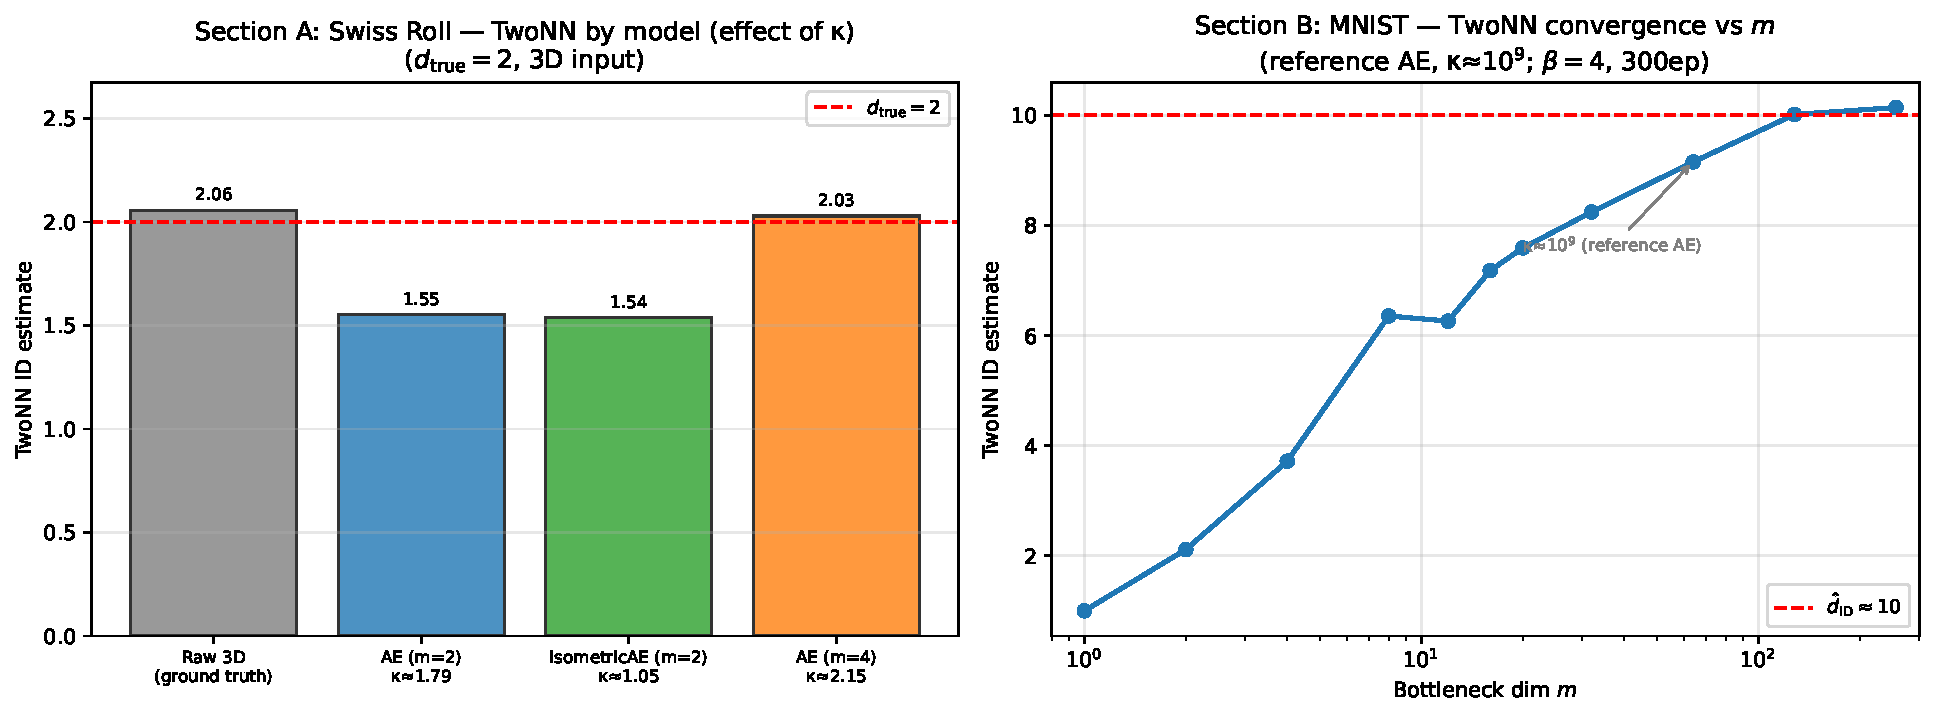
\includegraphics[width=0.95\linewidth]{results/figures/EP_twonn_stability.pdf}
  \caption{Exp-Stab/Exp-Geom: (Left) TwoNN ID on Swiss Roll --- AE and IsometricAE both underestimate at $m=d_\mathrm{true}$; TwoNN recovers at $m=4>d_\mathrm{true}$. (Right) MNIST AE $m$-sweep: TwoNN stabilizes at $m \geq 48$ despite $\kap$ jumping to $37.0$ at $m=128$. Detailed tables in Appendix D.}
  \label{fig:ep}
\end{figure}}{}
\subsection{MNIST: Reading Off the Effective Representation Dimensionality (Main Experiments, RQ1 and RQ2)}\label{sec:exp_mnist}

We validate the application of the proposed framework to real data using the MNIST dataset (main experiments).
MNIST provides a realistic evaluation environment for the framework in the sense that it is
``real data for which $\dtrue$ is unknown but $\hat{d}_\mathrm{ID}$ can be estimated.''

\subsubsection{Intrinsic-Dimension Estimation with an AE (Experiment Exp-Mnist-Base-AE)}

Table~\ref{tab:e4_ae} shows the results for the MNIST AE (300 epochs).

\begin{table}[H]
\centering
\caption{Exp-Mnist-Base: MNIST AE results (300 epochs, $n_\mathrm{train}=20{,}000$).}
\label{tab:e4_ae}
\small
\begin{tabular}{rcccc}
\toprule
$m$ & MSE & TwoNN ID & MLE ID & CKA \\
\midrule
1   & 0.0437 & 1.02  & 1.15  & 0.102 \\
4   & 0.0292 & 3.86  & 4.29  & 0.575 \\
8   & 0.0191 & 6.08  & 6.70  & 0.725 \\
16  & 0.0121 & 7.96  & 8.61  & 0.812 \\
32  & 0.0087 & 8.84  & 9.89  & 0.875 \\
64  & 0.0062 & 9.54  & 11.26 & 0.908 \\
128 & 0.0061 & 9.84  & 11.45 & 0.921 \\
256 & 0.0057 & \textbf{10.02} & \textbf{11.85} & 0.953 \\
\bottomrule
\end{tabular}
\end{table}

For $m \geq 64$, the TwoNN ID (9.54--10.02) and the MLE ID (11.26--11.85) converge,
indicating that the effective intrinsic dimension of MNIST lies roughly in the range
$\hat{d}_\mathrm{ID} \approx 10$--12.

\textbf{Comparison with linear PCA}:
Applying PCA to MNIST ($n = 20{,}000$) requires 43 dimensions to reach 80\% cumulative
explained variance and 86 dimensions to reach 90\%.
These values are 4--8 times larger than the AE-based estimate (TwoNN $\approx 10$),
demonstrating the nonlinear manifold structure of MNIST (see Figure~\ref{fig:e4_dualaxis}).

\subsubsection{VAE AU Dynamics and $\mknee$ (Experiment Exp-Mnist-Base-VAE)}

Table~\ref{tab:e4_vae} and Figure~\ref{fig:e4_dualaxis} show the AU pattern of the MNIST VAE
($\beta = 4$, 300 epochs).

\begin{table}[H]
\centering
\caption{Exp-Mnist-Base: MNIST VAE ($\beta=4$) results (300 epochs). AU increase rate slows at $m=12$ ($\mknee=12$).}
\label{tab:e4_vae}
\small
\begin{tabular}{rcccc}
\toprule
$m$ & MSE & AU & TwoNN ID & Change in $r(m)$ \\
\midrule
1   & 0.0464 & 1  & 1.00 & --- \\
4   & 0.0275 & 4  & 3.72 & normal growth \\
8   & 0.0186 & 8  & 6.36 & normal growth \\
\textbf{12} & 0.0184 & \textbf{8}  & 6.26 & \textbf{sharp drop} $\leftarrow \mknee = 12$ \\
16  & 0.0148 & 11 & 7.18 & low \\
20  & 0.0134 & 13 & 7.59 & low \\
32  & 0.0121 & 15 & 8.25 & low \\
64  & 0.0103 & 29 & 9.16 & gradual \\
128 & 0.0085 & 26 & 10.02 & gradual \\
256 & 0.0072 & 36 & 10.14 & gradual \\
\bottomrule
\end{tabular}
\end{table}

At $m = 12$, AU $= 8$ (the same value as at the preceding $m = 8$), and the AU increase rate
$r(m)$ drops sharply ($r(12) \approx 0$).
This triggers the threshold $\tau_{\mathrm{knee}} = 0.25$, and $\mknee = 12$ is observed.

\textbf{Caveat}: this value is a preliminary observation obtained with a single seed (seed 42)
and a specific extended grid ($m \in \{1,4,8,\ldots,256\}$); subsequent multi-seed experiments
(Sections~\ref{sec:exp_multiseed} and~\ref{sec:exp_multiseed2}) showed that it does not
reproduce with the same $m$ values and grid.
Although under the single-seed, extended-grid condition it happened to lie close to the TwoNN ID
range ($\approx 10$--12),
\textbf{in this paper we treat $\mknee = 10.3 \pm 0.9$ from Exp-Mnist-Dense-300 --- based on a
dense grid, independent initialization, and multiple seeds --- as the main stabilized result}
(Section~\ref{sec:exp_el}).

\IfFileExists{results/figures/E4_mnist_dualaxis.pdf}{%
\begin{figure}[H]
\centering
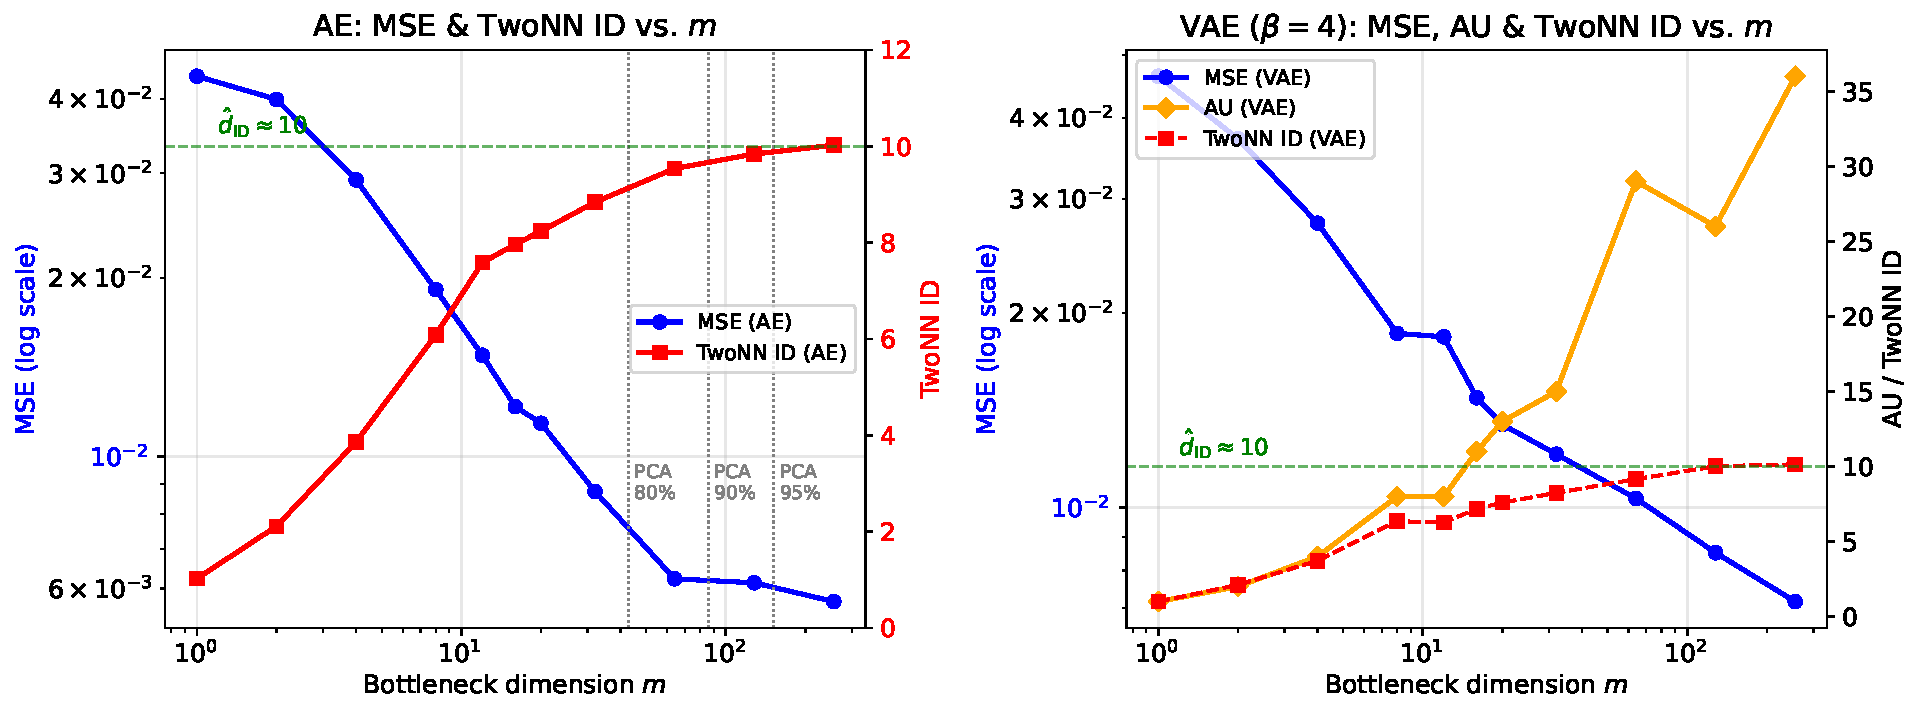
\includegraphics[width=0.95\linewidth]{results/figures/E4_mnist_dualaxis.pdf}
\caption{Exp-Mnist-Base: $m$-dependence of each indicator for MNIST (300 epochs). \textbf{Left (AE)}: MSE (log scale, left axis) and TwoNN ID (right axis). Vertical dotted lines correspond to PCA cumulative variance 80\% (43 dims), 90\% (86 dims), 95\% (152 dims); the difference from the nonlinear AE estimate (TwoNN $\approx 10$) is clear. \textbf{Right (VAE, $\beta=4$)}: MSE (log scale, left axis), AU (right axis), TwoNN ID (right axis, dashed). At $m = 12$ ($\mknee$), the AU increase rate drops sharply (arrow), indicating a heuristic slowdown point; the main stabilized result is $\mknee=10.3\pm0.9$ from Exp-Mnist-Dense-300 (Section~\ref{sec:exp_el}).}
\label{fig:e4_dualaxis}
\end{figure}}{}%

\subsubsection{Comparison with Existing Indicators}\label{sec:exp_comparison}

We compare the proposed indicator $\mknee$ with other representative indicators for choosing
the bottleneck dimension (Table~\ref{tab:method_comparison}).

\begin{table}[H]
\begin{adjustwidth}{-\extralength}{0cm}
\centering
\caption{Comparison of bottleneck dimension estimates on MNIST. $\mknee$ entries distinguish sparse-grid and dense-grid conditions.}
\label{tab:method_comparison}
\small
\begin{tabular}{p{4.0cm}cc p{4.5cm}}
\toprule
Method & Estimate & Source & Characteristics / Limitations \\
\midrule
PCA (80\% var.) & 43 & Exp-Mnist-Base-AE & Linear; overestimates nonlinear ID \\
PCA (90\% var.) & 86 & Exp-Mnist-Base-AE & Linear; larger overestimate \\
MSE elbow (AE) & $\approx16$--$20$ & Exp-Mnist-Base-AE & Intuitive; depends on smoothing \\
TwoNN ID (ref.\ AE) & $\approx10$--$12$ & Exp-Mnist-Base-AE & Nonlinear; subject to isometry bias \\
\midrule
$\mknee$ sparse-grid (3 seeds) & $43\pm15$ & Exp-Mnist-Multi-300 & Exploratory; unreliable at sparse grid \\
$\mknee$ \textbf{dense-grid (3 seeds)} & $\boldsymbol{10.3\pm0.9}$ & \textbf{Exp-Mnist-Dense-300} & \textbf{Exploratory; recommended for use} \\
\midrule
\multicolumn{4}{p{13.5cm}}{\footnotesize Dense-grid: $m\in\{8,9,\ldots,16,18,\ldots,64\}$ with independent initialization per $(m,\mathrm{seed})$. $\mknee=10.3\pm0.9$ aligns with TwoNN ID ($\approx10$). Sparse-grid $\mknee=43\pm15$ is unreliable as a diagnostic reference.} \\
\bottomrule
\end{tabular}
\end{adjustwidth}
\end{table}

Characteristics of each method:
PCA, being a linear method, cannot capture the nonlinear manifold structure of MNIST and
requires more than four times as many dimensions as the AE-based estimate (TwoNN $\approx 10$).
The MSE elbow is intuitive, but for a smooth MSE curve (cf.\ Exp-Mnist-Base) the location of
the elbow tends to be ambiguous.
TwoNN is effective as a nonlinear ID estimator but is subject to the isometry bias of the
reference AE.
$\mknee$ is complementary to these indicators in that it directly observes the KL dynamics;
however, it depends on $\tau$, $\beta$, and the $m$-grid, and is therefore best used within a
multi-indicator approach combined with the other indicators rather than in isolation.

\subsubsection{Multi-Seed Validation (Experiment Exp-Mnist-Multi-150)}\label{sec:exp_multiseed}

To assess the statistical reliability of $\mknee$, we repeated the MNIST VAE experiment
($\beta = 4$, 150 epochs, $m \in \{4,8,12,16,20,32,64\}$)
with three random seeds (42, 123, 777)
(experiment Exp-Mnist-Multi-150; Table~\ref{tab:e4_multiseed}).

\begin{table}[H]
\centering
\caption{Exp-Mnist-Multi-150: Mean$\pm$std of AU and TwoNN ID for 3 seeds (42, 123, 777) at 150 epochs ($\beta=4$). AU values are highly consistent across seeds, but $\mknee$ varies.}
\label{tab:e4_multiseed}
\small
\begin{tabular}{rccl}
\toprule
$m$ & AU (mean$\pm$std) & TwoNN ID (mean$\pm$std) & Note \\
\midrule
 4 & $4.0 \pm 0.0$ & $3.98 \pm 0.06$ & all dims active \\
 8 & $7.7 \pm 0.5$ & $6.37 \pm 0.41$ & \\
12 & $10.0 \pm 0.0$ & $7.35 \pm 0.19$ & \\
16 & $11.3 \pm 0.5$ & $7.66 \pm 0.18$ & \\
20 & $13.3 \pm 0.5$ & $8.31 \pm 0.18$ & \\
32 & $16.0 \pm 0.0$ & $8.92 \pm 0.14$ & \\
64 & $22.0 \pm 0.0$ & $9.94 \pm 0.08$ & converges to $\hat{d}_\mathrm{ID} \approx 10$ \\
\midrule
\multicolumn{4}{l}{$\mknee$ ($\tau=0.25$): seed 42 $=$ 64, seed 123 $=$ 32, seed 777 $=$ 64} \\
\multicolumn{4}{l}{Mean $\mknee = 53 \pm 15$ (150 epochs); the main result is the dense-grid,} \\
\multicolumn{4}{l}{independently initialized Exp-Mnist-Dense-300: $\mknee = 10.3 \pm 0.9$} \\
\bottomrule
\end{tabular}
\end{table}

\IfFileExists{results/figures/E4_multiseed.pdf}{%
\begin{figure}[H]
  \centering
  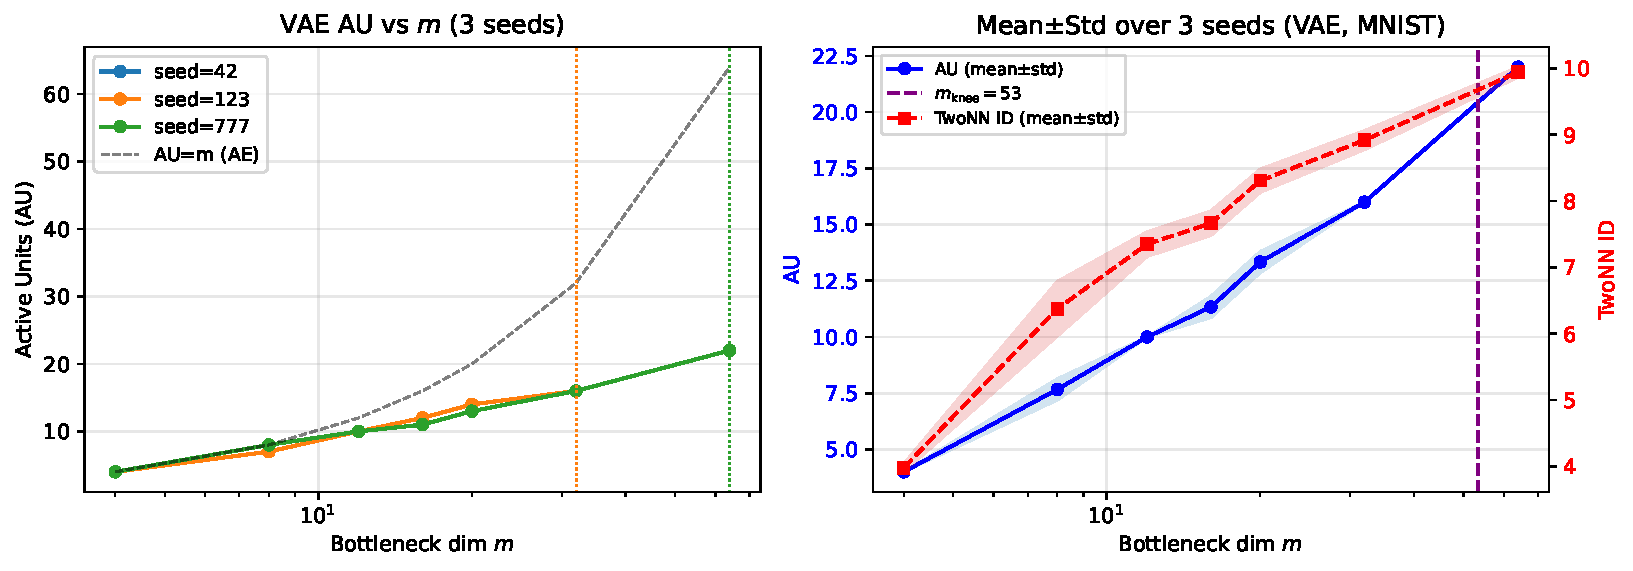
\includegraphics[width=0.9\linewidth]{results/figures/E4_multiseed.pdf}
  \caption{Exp-Mnist-Multi: AU patterns of MNIST VAE (3 seeds). Left: AU vs $m$ per seed (dotted lines: $\mknee$ per seed); Right: mean$\pm$std band. AU values are highly consistent across seeds, but $\mknee$ varies between 32 and 64.}
  \label{fig:e4_multiseed}
\end{figure}}{}

\textbf{Key findings}:
The AU values at each $m$ are highly consistent across the three seeds
($\sigma \leq 0.5$; Table~\ref{tab:e4_multiseed}).
The TwoNN ID also converges to $9.94 \pm 0.08$ at $m = 64$, confirming that the estimate
$\hat{d}_\mathrm{ID} \approx 10$ is seed-invariant.

In contrast, $\mknee$ ($\tau = 0.25$) varied across seeds: seed 42 $=$ 64, seed 123 $=$ 32,
seed 777 $=$ 64 (mean $53 \pm 15$).
This occurs because the AU increase rate $r(m)$ fluctuates subtly around the threshold
$\tau = 0.25$ at several $m$ values, and this instability is amplified under the incomplete
convergence of 150-epoch training.
Note that the extended Exp-Mnist-Base experiment (single seed 42) yielded $\mknee = 12$ at
300 epochs, but the instability persists in the 300-epoch multi-seed experiment described
below (Section~\ref{sec:exp_multiseed2}; mean $43 \pm 15$).
\textbf{Although insufficient convergence compounds the problem at 150 epochs, extending
training to 300 epochs does not restore the numerical stability of $\mknee$; the dominant
causes turn out to be the dependence on the $m$-grid and on the random seed}
(Section~\ref{sec:exp_multiseed2}).
This finding quantitatively substantiates the limitation stated in
Section~\ref{sec:disc_limitation}.

\subsubsection{300-Epoch Multi-Seed Validation (Experiment Exp-Mnist-Multi-300)}\label{sec:exp_multiseed2}

To test whether the $\mknee$ instability in the 150-epoch experiment was due to insufficient
convergence, we ran an experiment under the same conditions (MNIST VAE, $\beta = 4$,
$m \in \{4, 8, 12, 16, 20, 32, 64\}$) with the number of epochs extended to 300
(Exp-Mnist-Multi-300) for three seeds (42, 123, 777) (Table~\ref{tab:e4_300ep_multiseed}).

\begin{table}[H]
\centering
\caption{Exp-Mnist-Multi-300: Mean$\pm$std of AU and TwoNN ID for 3 seeds at 300 epochs ($\beta=4$). AU and TwoNN ID are highly consistent, but $\mknee$ still varies.}
\label{tab:e4_300ep_multiseed}
\small
\begin{tabular}{rccl}
\toprule
$m$ & AU (mean$\pm$std) & TwoNN ID (mean$\pm$std) & Note \\
\midrule
 4 & $4.0 \pm 0.0$ & $3.98 \pm 0.14$ & all dims active \\
 8 & $8.0 \pm 0.0$ & $6.67 \pm 0.15$ & \\
12 & $10.0 \pm 0.0$ & $7.41 \pm 0.06$ & \\
16 & $11.7 \pm 0.5$ & $7.95 \pm 0.21$ & AU still increasing \\
20 & $13.3 \pm 0.5$ & $8.37 \pm 0.14$ & \\
32 & $15.7 \pm 0.5$ & $9.07 \pm 0.10$ & \\
64 & $22.3 \pm 0.5$ & $10.03 \pm 0.12$ & converges to $\hat{d}_\mathrm{ID} \approx 10$ \\
\midrule
\multicolumn{4}{l}{$\mknee$ ($\tau=0.25$): seed 42 $=$ 64, seed 123 $=$ 32, seed 777 $=$ 32} \\
\multicolumn{4}{l}{Mean $\mknee = 43 \pm 15$ (300 epochs)} \\
\bottomrule
\end{tabular}
\end{table}

\IfFileExists{results/figures/E4_300ep_multiseed.pdf}{%
\begin{figure}[H]
  \centering
  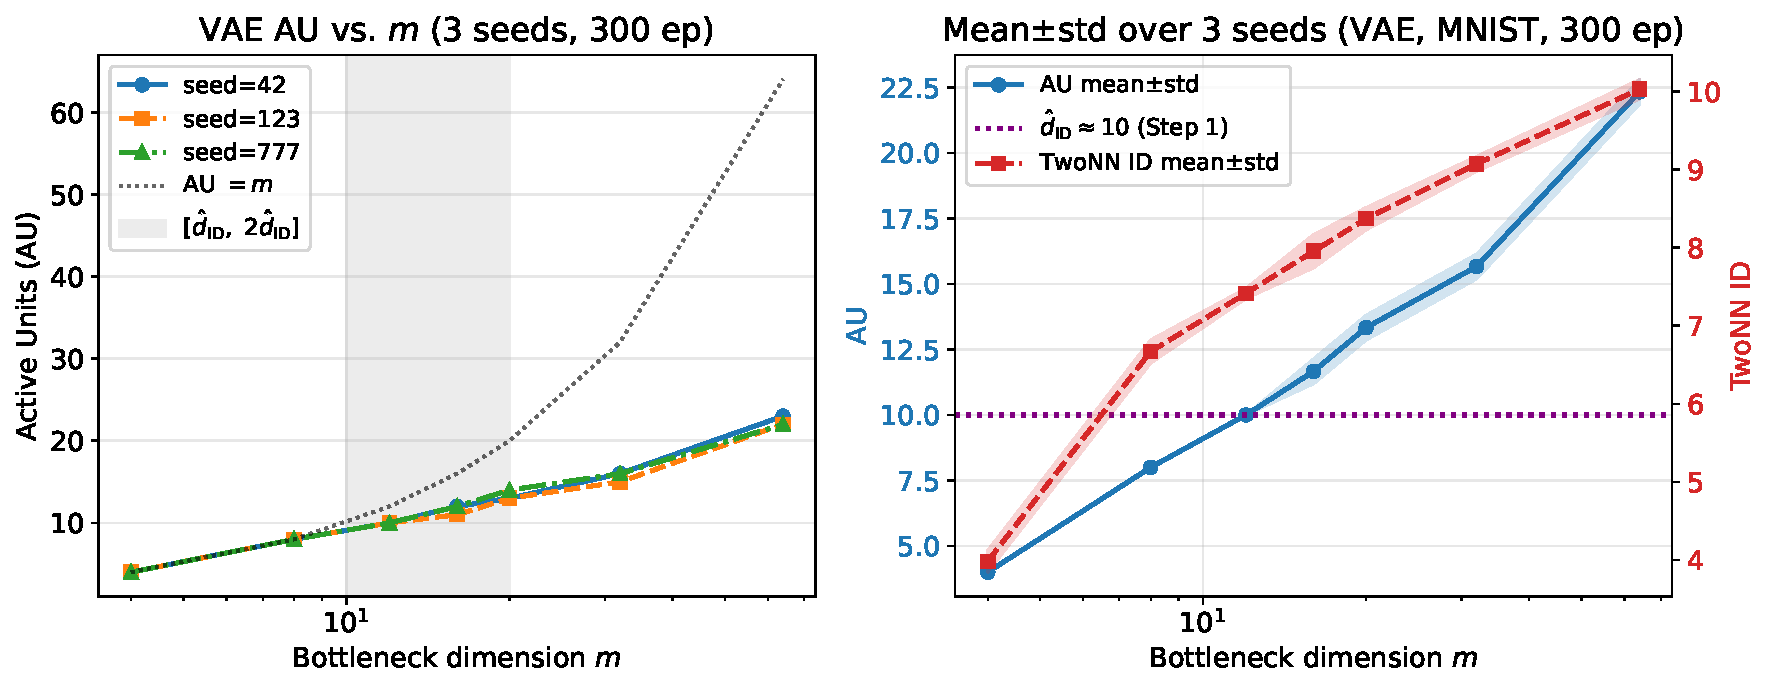
\includegraphics[width=0.9\linewidth]{results/figures/E4_300ep_multiseed.pdf}
  \caption{Exp-Mnist-Multi: AU patterns of MNIST VAE (3 seeds, 300 epochs). Left: AU vs $m$ per seed (dotted lines: $\mknee$); Right: mean$\pm$std band. AU and TwoNN ID bands are very narrow, but $\mknee$ varies between 32 and 64 across seeds.}
  \label{fig:e4_300ep_multiseed}
\end{figure}}{}

\textbf{Key findings}:
The AU values (Table~\ref{tab:e4_300ep_multiseed}) remain highly consistent across the three
seeds at 300 epochs ($\sigma \leq 0.5$), and the TwoNN ID is likewise stable at
$10.03 \pm 0.12$ for $m = 64$.
We thus confirmed that these quantitative indicators are robust to the seed and to the degree
of convergence.

In contrast, $\mknee$ still varied between 32 and 64 across seeds even under full 300-epoch
convergence (mean $43 \pm 15$).
This is essentially the same variation range as in Exp-Mnist-Multi-150
($\mknee = 32$--$64$), so extending training to 300 epochs did not resolve the instability of
$\mknee$.

Note that the $\mknee = 12$ obtained in the extended Exp-Mnist-Base experiment is a
preliminary observation that depends on the grid design and the initialization trajectory;
in this paper we adopt $\mknee = 10.3 \pm 0.9$ from Exp-Mnist-Dense-300 --- obtained under
independent initialization, multiple seeds, and a dense grid --- as the main result
(implementation details in Appendix~\ref{app:twonn_detail}).
\textbf{$\mknee$ is an exploratory change point derived from the AU growth curve, and its
value depends on the experimental setup (grid, seed, and initialization).}

\subsubsection{Linear Theory--Experiment Bridge (Experiment Exp-Mnist-PCA; Details in Appendix~\ref{app:twonn_detail})}\label{sec:exp_em}

Contrasting the MNIST PCA spectrum ($\lambda_1=5.22, \ldots, \lambda_{10}=1.23$) with
Theorem~\ref{thm:linear_vae}, we obtain $d^* \approx 10$ for
$\tau^2_\mathrm{eff} \approx 0.30$ (back-calculated), qualitatively consistent with the
observed TwoNN ID.
Whereas the linear setting produces a sharp saturation transition, in nonlinear VAEs gradient
competition yields a smooth, gradually increasing curve, which theoretically corroborates the
sparse-grid instability of $\mknee$ (detailed PCA spectrum tables and theory--experiment
comparison tables are given in Appendix~\ref{app:twonn_detail}).
For Conv-VAEs, the powerful reconstruction capability of the nonlinear decoder makes
$\tau^2_\mathrm{eff}$ even smaller, so the $m$ required for AU saturation increases
substantially relative to the FC-VAE (Section~\ref{sec:disc_convvae}).

\subsubsection{Dense-Grid $\times$ Seed $\times$ Epoch Factor-Isolation Experiment (Experiment Exp-Mnist-Dense)}\label{sec:exp_el}

To rigorously identify which factors cause the instability of $\mknee$, we designed an
experiment that isolates three factors: grid density, epochs, and seed.
Exp-Mnist-Base and Exp-Mnist-Multi already separate the epoch factor (150 ep vs.\ 300 ep) and
the seed factor (3 seeds).
The present experiment, Exp-Mnist-Dense, further isolates the grid-density factor: we trained
with $m \in \{8,9,10,11,12,13,14,15,16,18,20,24,28,32,40,48,64\}$
(17 points, adjacent spacing 1--8) for 300 epochs and 3 seeds.
The dense grid covers in particular $m = 8$--16 (around the estimated
$\hat{d}_\mathrm{ID} \approx 10$) in steps of 1
(Proposition~\ref{thm:mknee_instab} is an auxiliary upper bound for an idealized model; while
a step-1 dense grid may bring $\mknee$ close to $d^*$, AU fluctuations of the nonlinear VAE
can also drive the actual error beyond the bound).

\begin{table}[H]
\begin{adjustwidth}{-\extralength}{0cm}
\centering
\caption{Exp-Mnist-Dense: Comparison of $\mknee$ between dense and sparse grids ($\tau=0.25$, MNIST FC-VAE, $\beta=4$). Consistent with the grid-sensitivity bound of Proposition \ref{thm:mknee_instab}.}
\label{tab:el_mknee}
\small
\begin{tabular}{lccccc}
\toprule
Condition & Max.\ grid interval & seed=42 & seed=123 & seed=777 & Mean$\pm$std \\
\midrule
Sparse grid, 150ep (Exp-Mnist-Multi-150) & 32 & 64 & 32 & 64 & $53 \pm 15$ \\
Sparse grid, 300ep (Exp-Mnist-Multi-300) & 32 & 64 & 32 & 32 & $43 \pm 15$ \\
Dense grid, 300ep (Exp-Mnist-Dense-300) & 8 (step 1 for 8--16) & 11 & 9 & 11 & $10.3 \pm 0.9$ \\
\bottomrule
\end{tabular}
\end{adjustwidth}
\end{table}

\begin{table}[H]
\centering
\caption{Exp-Mnist-Dense: AU$(m)$ for dense grid (seed=42, 300ep, representative values).}
\label{tab:el_au}
\small
\begin{tabular}{rcccccccc}
\toprule
$m$ & 8 & 9 & 10 & 11 & 12 & 13 & 14 & 15 \\
\midrule
AU & 8 & 9 & 10 & 10 & 10 & 10 & 12 & 11 \\
\midrule
$m$ & 16 & 18 & 20 & 24 & 28 & 32 & 48 & 64 \\
\midrule
AU & 14 & 13 & 15 & 14 & 15 & 15 & 19 & 21 \\
\bottomrule
\end{tabular}
\end{table}

\IfFileExists{results/figures/EL_dense_grid_mknee.pdf}{%
\begin{figure}[H]
  \centering
  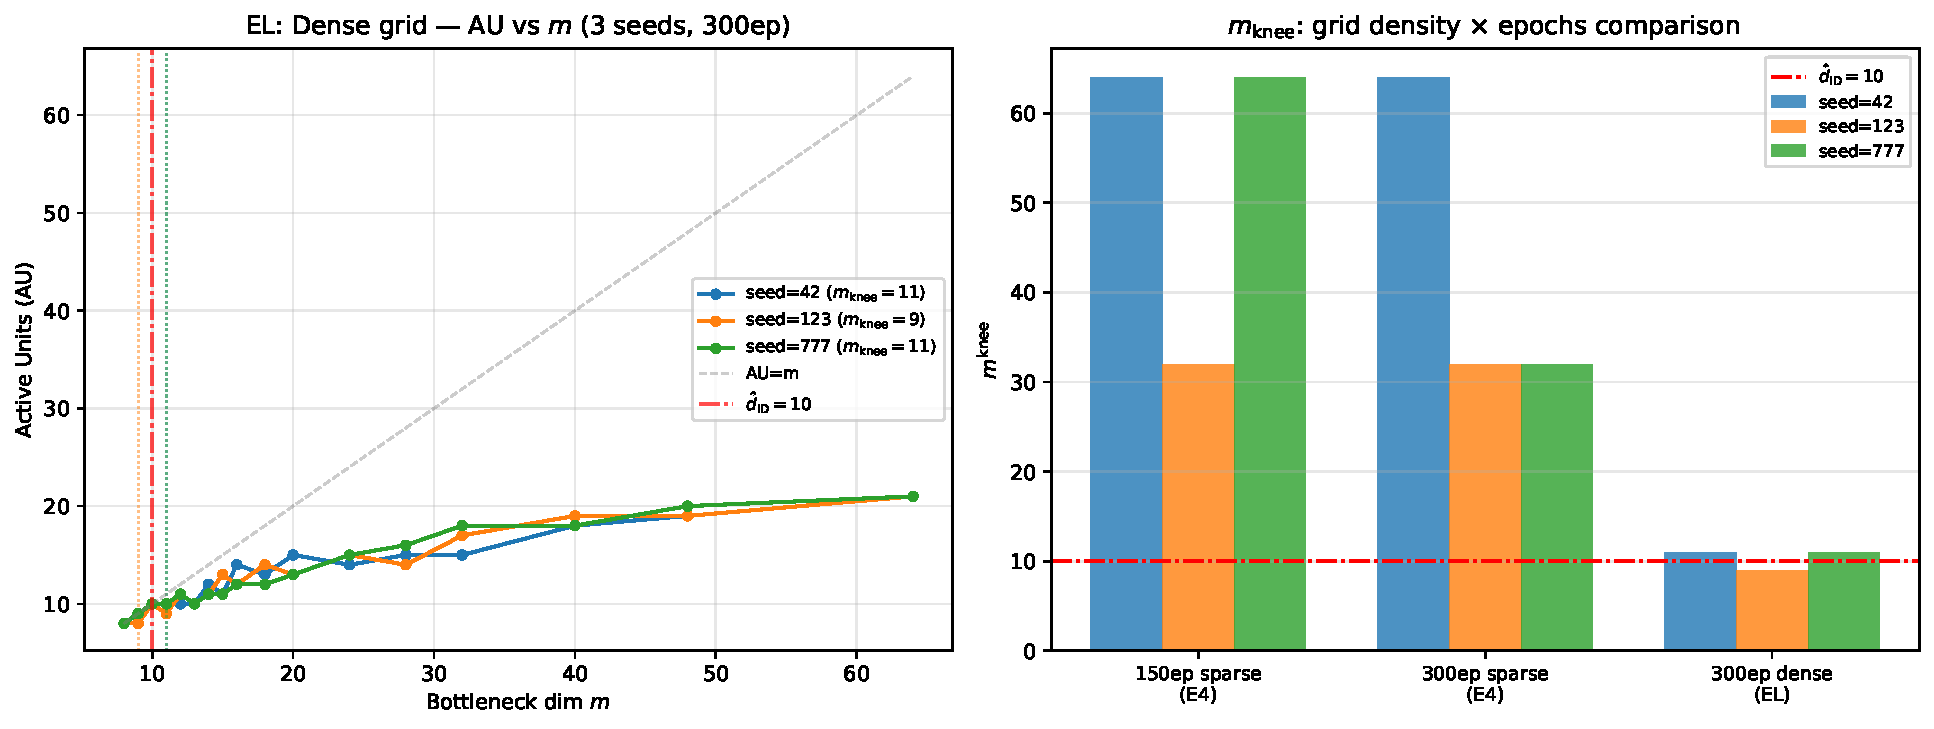
\includegraphics[width=0.95\linewidth]{results/figures/EL_dense_grid_mknee.pdf}
  \caption{Exp-Mnist-Dense: (Left) Dense-grid AU vs $m$ (3 seeds). (Right) Comparison by grid density $\times$ epochs. $\mknee$ variation in the dense grid can be assessed by the upper bound of Proposition~\ref{thm:mknee_instab} (maximum grid interval).}
  \label{fig:el}
\end{figure}}{}

\textbf{Significance of the Exp-Mnist-Dense experiment}:
The three-row comparison in Table~\ref{tab:el_mknee} quantitatively isolates the three
factors (grid density, epochs, and seed):
\begin{itemize}
  \item \textbf{Epoch factor}: sparse grid, 150 ep $\to$ 300 ep ($\mknee$: $53\pm15$ $\to$ $43\pm15$) --- increasing the epochs stabilizes $\mknee$ slightly, but is not the main cause
  \item \textbf{Seed factor}: variation across the 3 seeds under identical conditions ($\sigma = 15$) --- differences in optimization trajectories due to initialization matter, but this is a secondary factor that coexists with the sparse grid
  \item \textbf{Grid-density factor (one of the main causes)}: with the dense grid (Exp-Mnist-Dense), $\mknee = 10.3 \pm 0.9$ (seeds $=[11,9,11]$) --- a dramatic improvement over the sparse-grid $43\pm15$, consistent with the estimate $\hat{d}_\mathrm{ID} \approx 10$
\end{itemize}

\noindent
\textbf{Effect of grid density (comparison with the implication of Proposition~\ref{thm:mknee_instab})}:
Proposition~\ref{thm:mknee_instab} is an auxiliary upper bound for an idealized monotone
saturation model and does not apply directly to the empirical AU curves of nonlinear VAEs.
Nevertheless, densely probing the neighborhood of the estimated ID ($m = 8$--16) in steps of 1
yielded $\mknee \in \{9, 11\}$ (3 seeds), greatly reducing the deviation from the TwoNN ID
($\approx 10$).
This is qualitatively consistent with the implication of Proposition~2 --- demonstrated for
the idealized model --- that grid design matters.
However, since empirical AU curves exhibit non-monotone fluctuations
(e.g., AU$=10 \to 10 \to 10 \to 12 \to 11$ in Table~\ref{tab:el_au}), it is more accurate to
state this as the observation that ``densifying the grid greatly reduced the variance of the
empirical $\mknee$'' rather than to claim that the deviation ``stayed within the upper bound.''

\noindent
\textbf{Comparison of the $\tau$-method and the second-difference method}:
Besides the first-difference ratio method adopted in this paper ($\tau = 0.25$), $\mknee$ can
be detected by the \textbf{second-difference method}, which locates the point of maximum
curvature of the AU$(m)$ curve (Appendix~\ref{app:tau_knee}).
Table~\ref{tab:el_knee_compare} shows the comparison on the Exp-Mnist-Dense dense-grid data.

\begin{table}[H]
\centering
\caption{Exp-Mnist-Dense: Comparison of $\tau$-method ($\tau=0.25$) and second-difference method (d2) for $\mknee$ detection (dense grid, 300ep, 3 seeds).}
\label{tab:el_knee_compare}
\small
\begin{tabular}{lcccc}
\toprule
Method & seed=42 & seed=123 & seed=777 & Mean$\pm$std \\
\midrule
$\tau$-method ($\tau=0.25$) & 11 & 9  & 11 & $10.3 \pm 0.9$ \\
Second-difference method (d2) & 15 & 28 & 12 & $18.3 \pm 6.8$ \\
\midrule
\multicolumn{5}{l}{Reference: $\hat{d}_\mathrm{ID} \approx 10$ (TwoNN, $m=64$, 3-seed mean)} \\
\bottomrule
\end{tabular}
\end{table}

The $\tau$-method yields a mean of $10.3 \pm 0.9$, consistent with
$\hat{d}_\mathrm{ID} \approx 10$, with small seed-to-seed variation.
In contrast, the d2 method is sensitive to the discrete noise of AU$(m)$; for seed=123 it
deviated strongly to $\mknee = 28$ (in the transition region the AU curve fluctuates as
$8 \to 10 \to 9 \to 11 \to 10 \to 11 \to 13$, which perturbs the location of the maximum
second difference).
Therefore, \textbf{the $\tau$-method is the more stable choice for detecting $\mknee$ under
dense-grid conditions}, and we position the d2 method as an auxiliary tool for locating
global ``elbow'' candidates (see Appendix~\ref{app:tau_knee}).

Finally, the fact that the MNIST VAE reaches $\AUsat = 36$ ($m=256$), substantially exceeding
$\hat{d}_\mathrm{ID} \approx 10$--12 (the Manifold Entanglement hypothesis), and the
two-phase pattern of the training dynamics (Exp-Mnist-Dyn) are both single-seed, preliminary
observations; multi-seed validation of these is left for future work
(see Section~\ref{sec:disc_incidental}).
\subsection{Application to Fashion-MNIST (Experiment Exp-Fashion, Preliminary External Check)}\label{sec:exp_fashion}

Fashion-MNIST (10 clothing classes, $28\times28$) is positioned as a preliminary external check
of the framework's seed-reproducibility claims (the main experiments use MNIST with 3 seeds).
It is a single-seed (seed 42) confirmation, and we do not claim the same level of reproducibility
as for MNIST (3 seeds).

\begin{table}[H]
\centering
\caption{Exp-Fashion: Fashion-MNIST AE and VAE results (100 epochs, $n_\mathrm{train}=10{,}000$, representative $m$ values).}
\label{tab:ef}
\small
\begin{tabular}{rcccrcc}
\toprule
\multicolumn{3}{c}{AE} & \phantom{xx} & \multicolumn{3}{c}{VAE ($\beta=4$)} \\
\cmidrule{1-3}\cmidrule{5-7}
$m$ & MSE & TwoNN ID && $m$ & MSE & AU \\
\midrule
 4  & 0.01831 & 3.90 && 4  & 0.01955 & 4  \\
 8  & 0.01389 & 5.86 && 8  & 0.01721 & 6  \\
12  & 0.01230 & 7.58 && 12 & 0.01597 & 6  \\
16  & 0.01138 & 8.11 && 16 & 0.01570 & 7  \\
20  & 0.01077 & 8.45 && 20 & 0.01471 & 8  \\
32  & 0.01010 & 8.99 && 32 & 0.01418 & 9  \\
64  & 0.00981 & 9.39 && 64 & 0.01318 & 11 \\
256 & 0.01009 & 9.42 && 256& 0.01193 & 25 \\
\bottomrule
\end{tabular}
\end{table}

\begin{figure}[t]
  \centering
  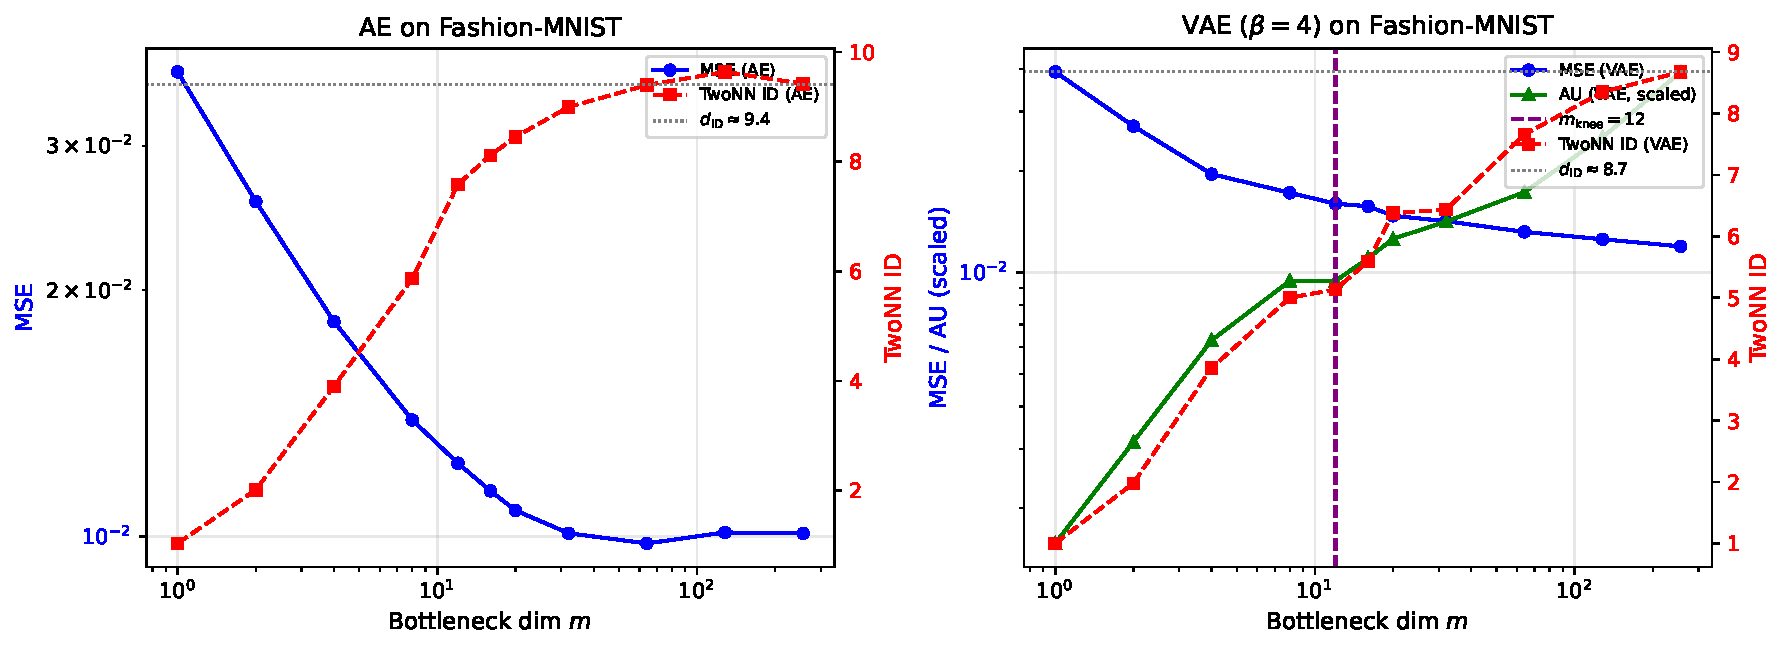
\includegraphics[width=0.9\linewidth]{results/figures/EF_fashion_mnist_dualaxis.pdf}
  \caption{Exp-Fashion: $m$-dependence of MSE, AU, and TwoNN ID for Fashion-MNIST AE (left) and VAE (right) (100 epochs). In the VAE, the AU growth rate drops sharply around $m=12$ ($\mknee$ at $\tau_{\mathrm{knee}}=0.25$), and TwoNN ID asymptotically converges to $\approx 9.4$ (AE) and $\approx 8.7$ (VAE) at $m \geq 32$.}
  \label{fig:ef}
\end{figure}

The results of Experiment Exp-Fashion (Table~\ref{tab:ef}, Figure~\ref{fig:ef}) yield the following findings.
For the AE, pseudo-AU $= m$ (essentially all latent coordinates are active) and TwoNN ID converges to
$\approx 9.4$ at $m \geq 32$, suggesting $\hat{d}_\mathrm{ID} \approx 9$--$10$ for Fashion-MNIST.
For the VAE ($\beta=4$, single seed), $\mknee = 12$ ($\tau_{\mathrm{knee}} = 0.25$) was observed;
however, this is an exploratory single-seed observation, and we note that it does not carry the
same level of reproducibility as the multi-seed sparse-grid result on MNIST ($\mknee = 43 \pm 15$).
AU remains at 25 even at $m = 256$ (unlike 36 for MNIST),
indicating that Fashion-MNIST may have a higher compression difficulty than MNIST.
The TwoNN ID estimates ($\approx 9$--$10$) are smaller than those for MNIST ($\approx 10$--$12$),
consistent with the intuition that clothing items have fewer local degrees of freedom than handwritten digits.

\subsection{Extension to Convolutional Architectures (Experiment Exp-Conv-AE)}\label{sec:exp_conv}

To address concerns about generalizability when the study is limited to fully connected architectures,
we conducted an experiment applying convolutional AE/VAE (Conv-AE/VAE) to MNIST (Experiment Exp-Conv-AE).

\textbf{Conv-AE/VAE architecture}:
\begin{itemize}
  \item Encoder: Conv($1\to32$, $k=3$, stride$=2$) $\to$ Conv($32\to64$, $k=3$, stride$=2$)
        $\to$ FC($3136\to m$) (for the VAE, $\to \mu, \log\sigma^2$)
  \item Decoder: FC($m\to3136$) $\to$ ConvT($64\to32$, $k=4$, stride$=2$) $\to$
        ConvT($32\to1$, $k=4$, stride$=2$) $\to$ Sigmoid
  \item $n_{\mathrm{train}} = 20{,}000$, 100 epochs, $m \in \{4, 8, 12, 16, 20, 32, 64\}$, seed 42
\end{itemize}

\begin{table}[H]
\centering
\caption{Exp-Conv-AE: MNIST Conv-AE and Conv-VAE ($\beta=4$) results (100 epochs, seed=42).}
\label{tab:eg}
\small
\begin{tabular}{rcc|rcc}
\toprule
\multicolumn{3}{c|}{Conv-AE} & \multicolumn{3}{c}{Conv-VAE ($\beta=4$)} \\
$m$ & MSE & TwoNN ID & $m$ & MSE & AU \\
\midrule
 4  & 0.0311 & 4.18  &  4  & 0.0331 &  4 \\
 8  & 0.0174 & 6.59  &  8  & 0.0197 &  8 \\
12  & 0.0113 & 7.80  & 12  & 0.0140 & 12 \\
16  & 0.0081 & 8.69  & 16  & 0.0109 & 16 \\
20  & 0.0069 & 9.03  & 20  & 0.0097 & 20 \\
32  & 0.0042 & 10.06 & 32  & 0.0070 & 32 \\
64  & 0.0020 & 11.29 & 64  & 0.0049 & 63 \\
\bottomrule
\end{tabular}
\end{table}

\IfFileExists{results/figures/EG_conv_mnist.pdf}{%
\begin{figure}[H]
  \centering
  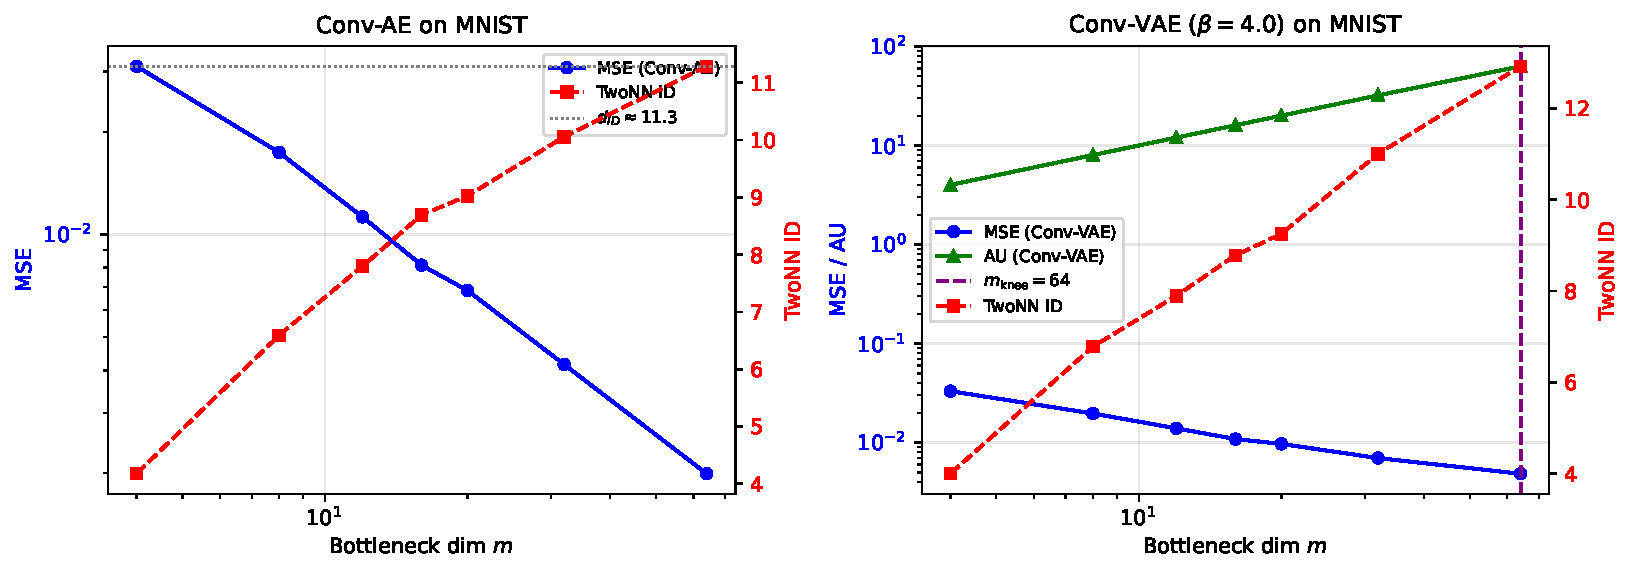
\includegraphics[width=0.9\linewidth]{results/figures/EG_conv_mnist.pdf}
  \caption{Exp-Conv-AE: $m$-dependence of MSE, AU, and TwoNN ID for MNIST Conv-AE (left) and Conv-VAE (right) (100 epochs). Conv-AE confirms AU$=m$ (all dims active) with TwoNN ID converging to $\approx 11$ at $m \geq 32$. Conv-VAE shows AU$\approx m$ (no saturation due to insufficient convergence at 100 epochs).}
  \label{fig:eg}
\end{figure}}{}

The results of Experiment Exp-Conv-AE (Table~\ref{tab:eg}) yield the following findings.

\textbf{TwoNN ID of the Conv-AE}: TwoNN ID converges to $11.29$ at $m = 64$,
consistent with the FC-AE estimate ($\approx 10$) (within an error of $\approx 10\%$).
We confirmed that the TwoNN ID estimates are consistent regardless of the architecture
(fully connected vs.\ convolutional)
(an empirical observation under the conditions of this study).

\textbf{Convergence sensitivity of the Conv-VAE}: AU $= m$ (no saturation) for $m \leq 32$ and AU $= 63$ at $m = 64$,
indicating that at 100 epochs the KL-regularization-driven dimension suppression is not yet functioning sufficiently.
This mirrors the 150-epoch FC-VAE experiment (Exp-Mnist-Multi: AU$\approx m$), and shows that
\textbf{reliable detection of $\mknee$ in Conv-VAEs also requires a larger number of epochs}.

\subsubsection{Delayed AU Saturation in Conv-VAEs: Fixed-$\beta$ vs.\ KL-Annealing Comparison (Experiments Exp-Conv-Fix and Exp-Conv-Ann)}
\label{sec:exp_conv_300ep}

Following the insufficient convergence in Exp-Conv-AE, we verified with 300 epochs and 3 seeds (Exp-Conv-Fix)
and with KL cyclic annealing (Exp-Conv-Ann)
(Table~\ref{tab:eh_conv_vae}).

\begin{table}[H]
\begin{adjustwidth}{-\extralength}{0cm}
\centering
\caption{Exp-Conv-Fix and Exp-Conv-Ann: Comparison of AU for MNIST Conv-VAE (300ep, mean$\pm$std over 3 seeds). FC-VAE (Exp-Mnist-Multi) saturates at $m=32$ (AU$=15.7$), while Conv-VAE shows AU$=m$ (no saturation) under both fixed-$\beta$ and annealing at $m \leq 32$.}
\label{tab:eh_conv_vae}
\small
\begin{tabular}{r ccc cc}
\toprule
 & \multicolumn{2}{c}{Conv-VAE fixed-$\beta$ (Exp-Conv-Fix)} & \multicolumn{1}{c}{Conv-VAE annealing (Exp-Conv-Ann)} & \multicolumn{2}{c}{FC-VAE (Exp-Mnist-Base, 300ep)} \\
$m$ & AU & TwoNN ID & AU & AU & TwoNN ID \\
\midrule
 4 & $4.0\pm0.0$ & $3.97\pm0.08$ & $4.0\pm0.0$ & $4.0$ & $3.98$ \\
12 & $12.0\pm0.0$ & $8.14\pm0.09$ & $12.0\pm0.0$ & $10.0$ & $7.41$ \\
32 & $32.0\pm0.0$ & $11.43\pm0.08$ & $32.0\pm0.0$ & $15.7$ & $9.07$ \\
64 & $54.3\pm0.5$ & $13.10\pm0.05$ & $64.0\pm0.0$ & $22.3$ & $10.03$ \\
\midrule
\multicolumn{6}{l}{$\mknee$: Conv-VAE (both conditions) all seeds $=64$ (grid upper bound); FC-VAE $=43\pm15$ (32--64)} \\
\bottomrule
\end{tabular}
\end{adjustwidth}
\end{table}

The Conv-VAE exhibits AU$=m$ (no saturation) for $m \leq 32$ under both fixed $\beta=4$ and cyclic annealing,
making the divergence from the FC-VAE clear (theoretical discussion in \S\ref{sec:disc_convvae}).
AU$\approx m$ is a signal that "KL regularization is not yet functioning," and in this state the TwoNN ID
is also inflated (Conv-VAE $m=64$: $13.10$ vs.\ FC-VAE: $10.03$).
\textbf{On the grid $m \leq 64$, AU saturation cannot be observed}, and an extension of the $m$ range is required.

%% ===================================================================
\subsection{Conv-VAE Extended $m$-Grid Experiments (Experiments Exp-Conv-M256 and Exp-Conv-M512)}\label{sec:exp_en}

Since no AU saturation was observed for $m \leq 64$ in Exp-Conv-Fix and Exp-Conv-Ann (\S\ref{sec:exp_conv_300ep}),
we extended the $m$ grid to 256 (Experiment Exp-Conv-M256) and 512 (Experiment Exp-Conv-M512).
Under the reduced-$\tau^2_\mathrm{eff}$ hypothesis discussed in \S\ref{sec:disc_convvae},
the Conv-VAE's $d^*(\beta)$ is substantially larger than that of the FC-VAE ($\approx 10$),
so a slowdown of AU growth is predicted to appear in the region $m>64$.

\textbf{Experimental setup} (Exp-Conv-M256):
Using the same Conv-VAE architecture as Exp-Conv-Ann ($28\times28$ MNIST, 2-layer Conv encoder,
2-layer ConvTranspose decoder, KL cyclic annealing with $\beta_\mathrm{max}=4$, 3 cycles,
150 epochs, seeds$\in\{42,123,777\}$),
we tested $m \in \{4, 8, 16, 32, 64, 96, 128, 192, 256\}$ (9 points).

\begin{table}[H]
\centering
\caption{Exp-Conv-M256: Conv-VAE extended $m$ grid (KL annealing, 150 epochs, mean$\pm$std, 3 seeds). AU$=m$ for $m \leq 64$; AU$<m$ begins at $m \geq 96$. FC-VAE reference (Exp-Mnist-Base, 300ep, $m=64$): AU$=22.3\pm0.5$.}
\label{tab:en}
\small
\begin{tabular}{rccc}
\toprule
$m$ & AU (mean$\pm$std) & TwoNN ID (mean$\pm$std) & Note \\
\midrule
  4 & $4.0\pm0.0$   & $3.84\pm0.11$ & all dims active \\
  8 & $8.0\pm0.0$   & $6.64\pm0.11$ & \\
 16 & $16.0\pm0.0$  & $8.76\pm0.05$ & \\
 32 & $32.0\pm0.0$  & $10.46\pm0.13$ & \\
 64 & $64.0\pm0.0$  & $13.29\pm0.12$ & same as Exp-Conv-Ann (no saturation) \\
 96 & $\mathbf{90.7\pm1.2}$  & $14.30\pm0.22$ & \textbf{AU$<m$ onset} (FC-VAE $\hat{d}_\mathrm{ID} \approx 9\times$) \\
128 & $111.7\pm2.6$ & $14.69\pm0.13$ & \\
192 & $159.0\pm4.3$ & $15.89\pm0.27$ & \\
256 & $241.3\pm2.9$ & $16.58\pm0.16$ & \\
\midrule
\multicolumn{4}{l}{$\mknee$ ($\tau=0.25$): all seeds $=256$ (no knee within the tested range)} \\
\multicolumn{4}{l}{FC-VAE reference (Exp-Mnist-Base, 300ep, $m=64$): AU$=22.3\pm0.5$, TwoNN ID$=10.03\pm0.12$} \\
\bottomrule
\end{tabular}
\end{table}

\IfFileExists{results/figures/EN_conv_vae_extended_m.pdf}{%
\begin{figure}[H]
  \centering
  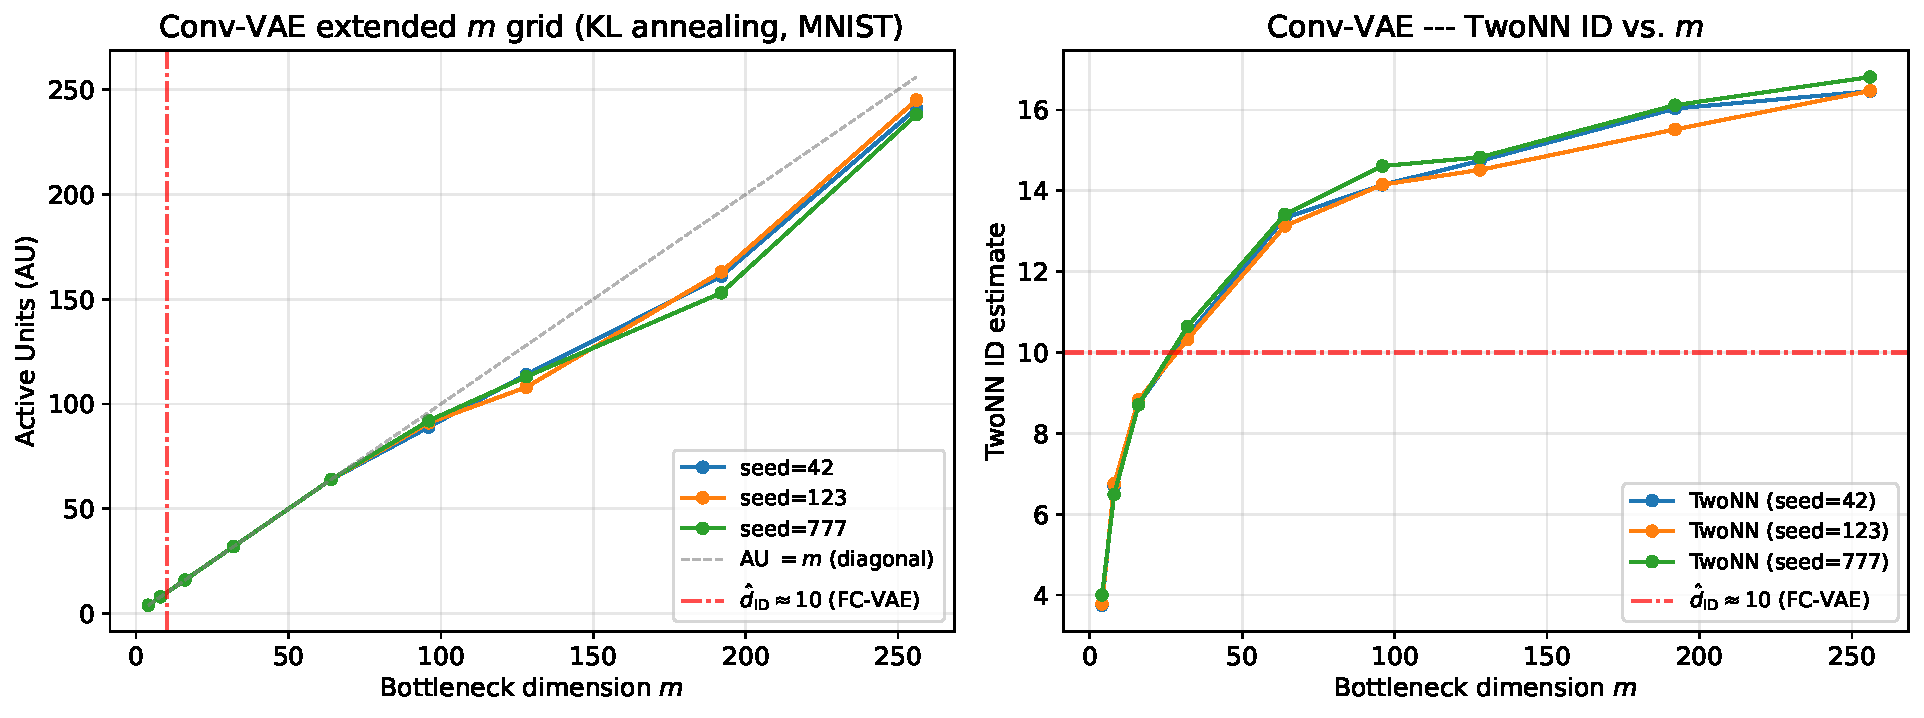
\includegraphics[width=0.95\linewidth]{results/figures/EN_conv_vae_extended_m.pdf}
  \caption{Exp-Conv-M256: Conv-VAE extended $m$ grid ($m\in[4,256]$, KL annealing, 3 seeds). AU vs $m$ (left) and TwoNN ID vs $m$ (right). Diagonal line (AU$=m$) and FC-VAE reference $\hat{d}_\mathrm{ID} \approx 10$ (red) are shown. AU$=m$ continues at $m \leq 64$ but deviates from the diagonal at $m \geq 96$, confirming qualitative water-filling behavior in Conv-VAE.}
  \label{fig:en}
\end{figure}}{}

\textbf{Main findings of Experiment Exp-Conv-M256}:
For $m \leq 64$, AU$=m$ holds consistently across all 3 seeds, making the contrast with the FC-VAE
($m=64$: AU$=22.3$) striking.
At $m = 96$, AU$=90.7\pm1.2$ ($<96$) appears, confirming the onset of a saturation trend
(standard deviation across 3 seeds $\sigma=1.2$).
At $m=256$, AU$=241.3\pm2.9$ (activation rate 94.3\%), still maintaining a high activation rate.
$\mknee$ ($\tau=0.25$) equals 256 for all 3 seeds, i.e., no sharp AU-saturation knee was found within
the tested range.
This result indicates that the Conv-VAE's $d^*(\beta)$ is substantially larger than the FC-VAE's
$d^*(\beta) \approx 10$ ($\gg 64$, likely $> 256$).
The correspondence with the $\tau^2_\mathrm{eff}$ theory and the implications for natural images
are discussed in \S\ref{sec:disc_convvae}.

\textbf{Extension beyond $m=256$ (Experiment Exp-Conv-M512, details in Appendix~\ref{app:convvae_natimg})}:
Even when extending to $m \in \{384, 512\}$, AU$\approx m$ (all dimensions active) is maintained across
all 3 seeds, and $\mknee$ remains pinned to the grid boundary at 512
(see Appendix~\ref{app:convvae_natimg} and its table).
This shows that the $d^*(\beta)$ of the MNIST Conv-VAE exceeds $m=512$,
consistent with the $\tau^2_\mathrm{eff}$ theoretical prediction of \S\ref{sec:disc_convvae}.
In the next subsection, we show that AU saturation can be artificially induced by strengthening $\beta_{\max}$.

%% ===================================================================
\subsection{Artificially Inducing Conv-VAE AU Saturation with High $\beta$ (Experiment Exp-ConvV-HiBeta)}\label{sec:exp_hibeta}

As a verification of the $\tau^2_\mathrm{eff}$ hypothesis of \S\ref{sec:disc_convvae}
(a powerful decoder pushes AU saturation toward higher dimensions),
we increased $\beta_{\max}$ from $4$ to $\{10, 20\}$ and checked whether an AU saturation plateau
is induced in the MNIST Conv-VAE.

\textbf{Experimental setup}: Using the same architecture and KL cyclic annealing (3 cycles) as Exp-Conv-M256,
we trained with $\beta_{\max} \in \{10, 20\}$, $m \in \{16, 32, 64, 96, 128, 192, 256\}$,
seed=42, and 150 epochs (the $\beta_{\max}=4$, seed=42 results of Exp-Conv-M256 are reproduced for comparison).

\begin{table}[H]
\centering
\caption{Exp-ConvV-HiBeta: Comparison of MNIST Conv-VAE AU at $\beta_\mathrm{max} \in \{4, 10, 20\}$ (seed=42, 150ep, KL cyclic annealing). Higher $\beta_\mathrm{max}$ induces AU saturation at lower dimensions.}
\label{tab:hibeta}
\small
\begin{tabular}{r ccc}
\toprule
$m$ & $\beta_{\max}=4$ (Exp-Conv-M256) & $\beta_{\max}=10$ & $\beta_{\max}=20$ \\
\midrule
 16  & 16  (100\%)& 16 (100\%) & 16 (100\%) \\
 32  & 32  (100\%)& 32 (100\%) & 27 (84\%)  \\
 64  & 64  (100\%)& 54 (84\%)  & 42 (66\%)  \\
 96  & 89  (93\%) & 65 (68\%)  & 47 (49\%)  \\
128  & 114 (89\%) & 69 (54\%)  & 53 (41\%)  \\
192  & 161 (84\%) & 79 (41\%)  & 60 (31\%)  \\
256  & 241 (94\%) & 93 (36\%)  & 66 (26\%)  \\
\midrule
$\mknee$ ($\tau=0.25$) & 512 (grid boundary, unidentified) & $\approx 128$ & $\approx 96$ \\
\bottomrule
\end{tabular}
\end{table}

\textbf{Findings of Exp-ConvV-HiBeta} (Table~\ref{tab:hibeta}):
Whereas at $\beta_{\max}=4$ AU$=m$ (100\% active) persists for $m \leq 64$,
at $\beta_{\max}=10$ a clear AU saturation trend appears --- AU$=54$ (84\%) at $m=64$,
AU$=69$ (54\%) at $m=128$, and AU$=93$ (36\%) at $m=256$ ---
and $\mknee \approx 128$ ($\tau=0.25$) was identified.
Furthermore, at $\beta_{\max}=20$, saturation occurs at even lower dimensions ---
AU$=27$ (84\%) at $m=32$ and AU$=42$ (66\%) at $m=64$ --- and $\mknee \approx 96$ was observed.
This directly matches the prediction of the $\tau^2_\mathrm{eff}$ hypothesis of \S\ref{sec:disc_convvae}:
increasing $\beta$ shifts $d^*(\beta) = |\{j: \lambda_j > \beta\tau^2_\mathrm{eff}\}|$ to smaller values,
and AU saturation appears at lower dimensions.
\textbf{This result is consistent with the interpretation that the absence of observed AU saturation
in the MNIST Conv-VAE is not an "applicability limit of the framework," but rather stems from the fact
that at the setting $\beta_{\max}=4$ the regularization was insufficient relative to the decoder capacity,
resulting in $d^*(\beta) \gg 256$.}
Applying the AU/$\mknee$ framework to Conv-VAEs requires an appropriate setting of $\beta$
matched to the data and architecture.

\IfFileExists{results/figures/Exp_ConvV_HiBeta.pdf}{%
\begin{figure}[H]
\centering
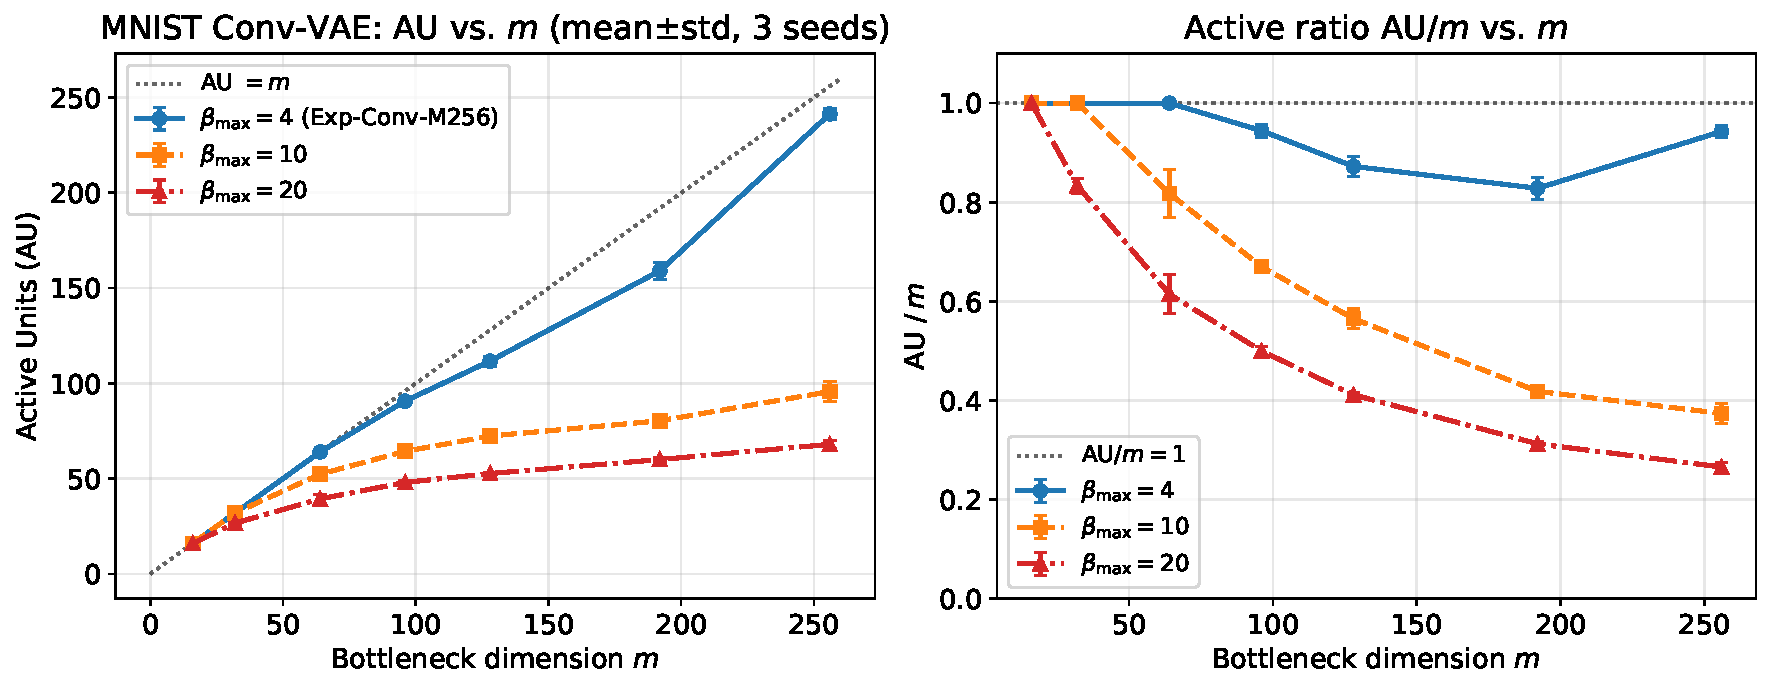
\includegraphics[width=0.9\linewidth]{results/figures/Exp_ConvV_HiBeta.pdf}
\caption{Exp-ConvV-HiBeta: Comparison of MNIST Conv-VAE AU vs $m$ (left) and activation rate AU/$m$ (right) for $\beta_{\max} \in \{4, 10, 20\}$. Increasing $\beta_{\max}$ shifts AU saturation to lower dimensions, demonstrating the $\beta$-dependence of $d^*(\beta)$.}
\label{fig:hibeta}
\end{figure}
}{}

%% ===================================================================
\subsection{Application to Natural Images: CIFAR-10 and SVHN (Experiments Exp-Nat-Cifar and Exp-Nat-SVHN)}\label{sec:exp_natural}

We applied the proposed framework to the more complex natural-image datasets
CIFAR-10~\cite{krizhevsky2009learning} and SVHN~\cite{netzer2011reading},
and compared the results with the intrinsic-dimension estimates reported by
Pope et al.~\cite{pope2021intrinsic}.

\textbf{Experimental setup} (Exp-Nat-Cifar: CIFAR-10; Exp-Nat-SVHN: SVHN):
\begin{itemize}
  \item Architecture: Conv-VAE (input $32 \times 32 \times 3$)
        \begin{itemize}
          \item Encoder: Conv($3\to32$, $k=4$, s$=2$, p$=1$) $\to$ Conv($32\to64$, $k=4$, s$=2$, p$=1$) $\to$
                Conv($64\to128$, $k=4$, s$=2$, p$=1$) $\to$ FC($2048 \to m$) $\times 2$ ($\mu$, $\log\sigma^2$)
          \item Decoder: FC($m \to 2048$) $\to$ ConvT($128\to64$) $\to$ ConvT($64\to32$) $\to$ ConvT($32\to3$) $\to$ Sigmoid
        \end{itemize}
  \item $n_{\mathrm{train}} = 20{,}000$, 150 epochs, KL cyclic annealing ($\beta_{\max}=4$, 3 cycles)
  \item $m \in \{16, 32, 64, 128, 256\}$, seeds $\in \{42, 123, 777\}$
\end{itemize}

\begin{table}[H]
\begin{adjustwidth}{-\extralength}{0cm}
\centering
\caption{Exp-Nat-Cifar and Exp-Nat-SVHN: Conv-VAE results for CIFAR-10 (left) and SVHN (right) (mean$\pm$std, 3 seeds; KL cyclic annealing, 150 epochs, 3 cycles). At $m=64$, CIFAR-10 latent TwoNN ID converges to the raw-data value ($\approx25$), consistent with Pope et al.\ \cite{pope2021intrinsic} ($d_\mathrm{ID} \approx 26$).}
\label{tab:ei_ej}
\small
\begin{tabular}{r cc | cc}
\toprule
 & \multicolumn{2}{c|}{CIFAR-10 (Exp-Nat-Cifar)} & \multicolumn{2}{c}{SVHN (Exp-Nat-SVHN)} \\
$m$ & AU (mean$\pm$std) & TwoNN ID (mean$\pm$std) & AU (mean$\pm$std) & TwoNN ID (mean$\pm$std) \\
\midrule
 16  & $16.0\pm0.0$ & $13.12\pm0.12$ & $16.0\pm0.0$ & $11.30\pm0.12$ \\
 32  & $32.0\pm0.0$ & $19.26\pm0.23$ & $32.0\pm0.0$ & $15.08\pm0.08$ \\
 64  & $64.0\pm0.0$ & $\mathbf{25.21\pm0.41}$ & $64.0\pm0.0$ & $19.97\pm0.12$ \\
128  & $128.0\pm0.0$ & $28.83\pm0.41$ & $125.3\pm0.5$ & $24.60\pm0.36$ \\
256  & $256.0\pm0.0$ & $30.91\pm0.64$ & $206.7\pm1.2$ & $27.08\pm0.34$ \\
\midrule
\multicolumn{3}{l|}{Raw TwoNN=25.20, MLE=26.56 ($\approx$ Pope et al.\ estimate of 26)} & \multicolumn{2}{l}{Raw TwoNN=10.09, MLE=18.85} \\
\multicolumn{3}{l|}{$\mknee$ ($\tau=0.25$): all seeds=256 (no knee in range)} & \multicolumn{2}{l}{$\mknee$: all seeds=256 (no knee in range)} \\
\bottomrule
\end{tabular}
\end{adjustwidth}
\end{table}

\IfFileExists{results/figures/EI_cifar10_conv_vae.pdf}{%
\begin{figure}[H]
  \centering
  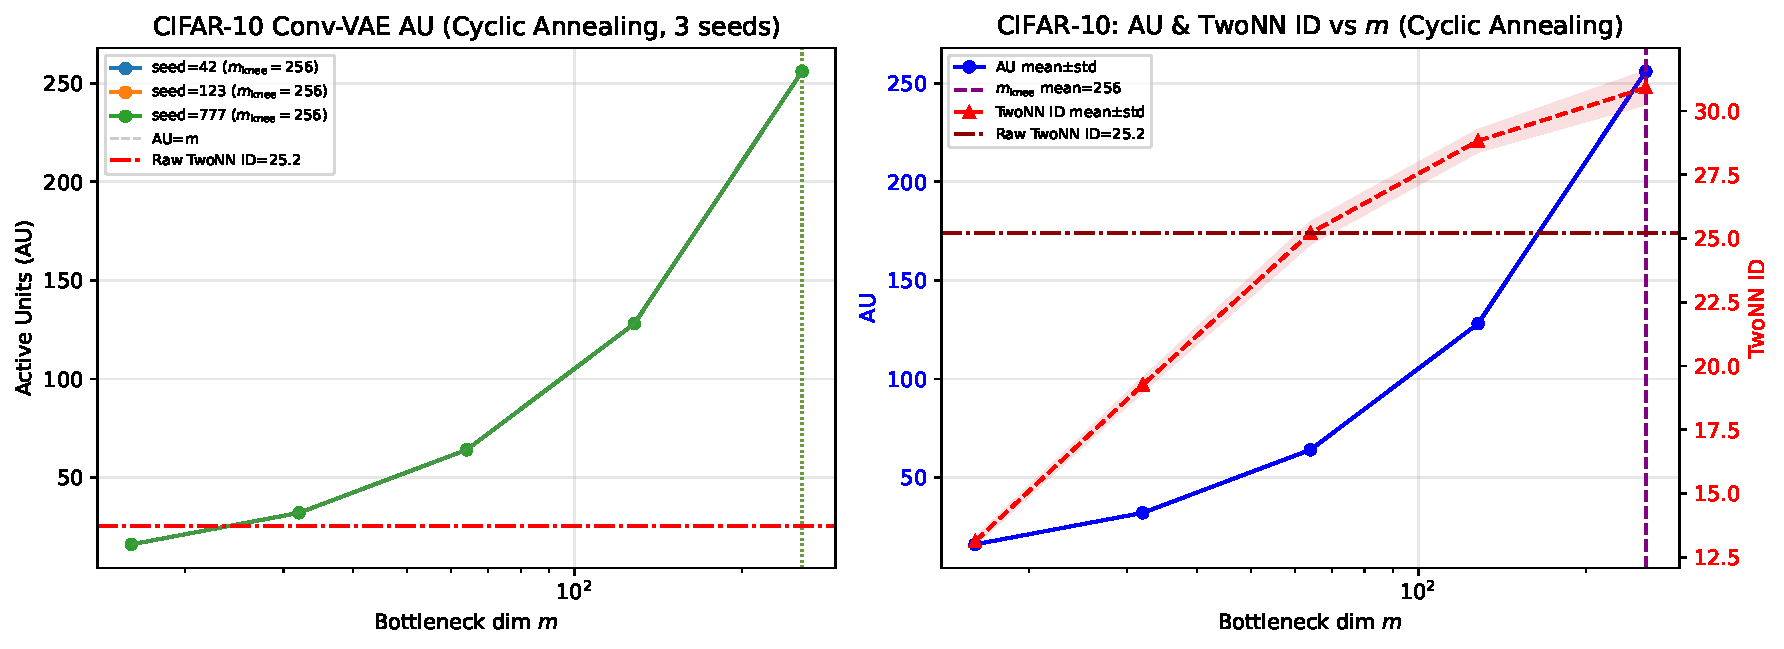
\includegraphics[width=0.95\linewidth]{results/figures/EI_cifar10_conv_vae.pdf}
  \caption{Exp-Nat-Cifar: $m$-dependence of AU and TwoNN ID for CIFAR-10 Conv-VAE (KL cyclic annealing, 3 seeds). TwoNN ID shows convergence consistent with Pope et al.\cite{pope2021intrinsic} ($d_\mathrm{ID} \approx 26$).}
  \label{fig:ei}
\end{figure}}{}

\IfFileExists{results/figures/EJ_svhn_conv_vae.pdf}{%
\begin{figure}[H]
  \centering
  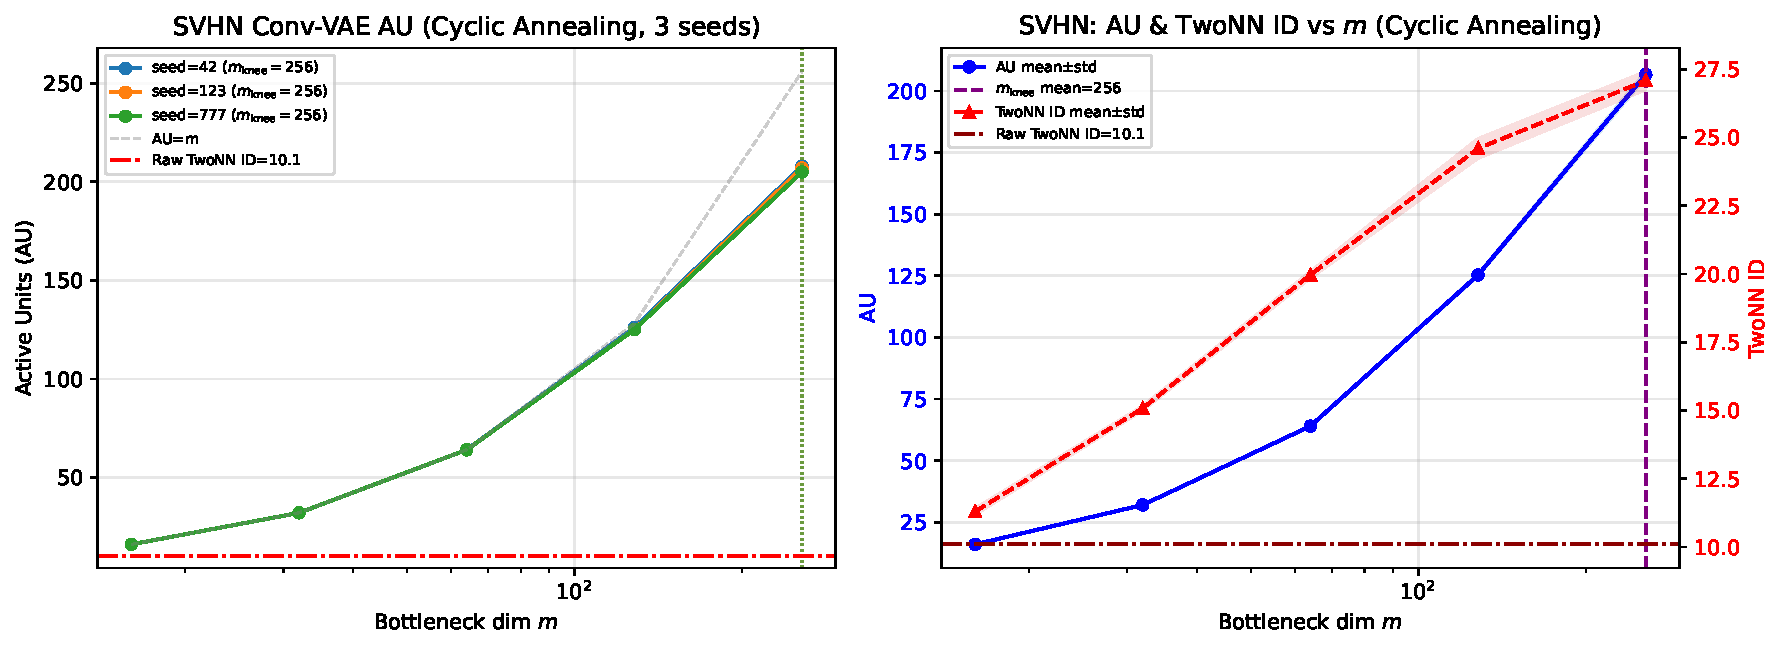
\includegraphics[width=0.95\linewidth]{results/figures/EJ_svhn_conv_vae.pdf}
  \caption{Exp-Nat-SVHN: $m$-dependence of AU and TwoNN ID for SVHN Conv-VAE (KL cyclic annealing, 3 seeds).}
  \label{fig:ej}
\end{figure}}{}

The primary aim of this experiment is limited to verifying whether the TwoNN ID
attains the same scale as the values reported by Pope et al.\ within an
appropriate bottleneck range (stable identification on the AU/$\mknee$ side is
left for future work).

\textbf{CIFAR-10 (Exp-Nat-Cifar) --- partial consistency check for TwoNN}:
the latent TwoNN ID at $m=64$, $25.21\pm0.41$ (3 seeds, $\sigma=0.41$),
is consistent with the raw-data TwoNN ID (25.20), yielding an estimate on the
same scale as the value reported by Pope et al.~\cite{pope2021intrinsic}
($\approx 26$) (Table~\ref{tab:ei_ej}).
However, the TwoNN ID rises to $28.83$ at $m=128$ and to $30.91$ at $m=256$,
so the ``consistency'' of the TwoNN ID is restricted to an appropriate
bottleneck range of roughly $m \approx 2\hat{d}_\mathrm{ID}$.
AU satisfies AU$=m$ for $m \leq 256$ (no saturation), and $\mknee$ equals 256
(the grid boundary) for all seeds.
Hence, this experiment demonstrates ``partial consistency of TwoNN within an
appropriate bottleneck range'' and does not claim generalization of the entire
framework to natural images.

\textbf{SVHN (Exp-Nat-SVHN) --- geometric distortion of the latent space}:
although AU$<m$ was observed for $m \geq 128$ ($m=256$: AU$=206.7\pm1.2$),
the latent TwoNN ID rises to $27.08$ at $m=256$, a large divergence from the
raw-data TwoNN of $10.09$.
This indicates that when AU uses all dimensions, the latent space may fail to
preserve isometry and the ID may be overestimated; it is therefore more
appropriately interpreted as geometric distortion of the latent space rather
than ``partial collapse.''
An AU saturation plateau is not reached, and this experiment illustrates one
instance of the applicability limits of the framework.

\subsection{Exploring AU Saturation Conditions in CIFAR-10 Conv-VAE (Experiment Exp-NatImg-AU)}\label{sec:exp_natimg_au}

\textbf{Positioning}: this section and \S\ref{sec:exp_natimg_sweep} are framed
as ``quantification of the applicability boundary'' experiments---rather than
reporting a failure of stable AU/$\mknee$ identification, they constitute a
set of experiments that systematically identify the boundary conditions under
which AU diagnostics become difficult.

The previous section (Exp-Nat-Cifar) used only a single setting with
$\beta_{\max}=4$ and 150 epochs; three factors are conceivable for the absence
of observed AU saturation: ``insufficient $\beta$,'' ``insufficient training,''
and ``insufficient architectural capacity.''
In this experiment, we systematically varied $\beta_{\max}$ and the
architecture depth to explore the conditions under which AU saturation becomes
detectable in a CIFAR-10 Conv-VAE.

\textbf{Experimental setup} (Exp-NatImg-AU):
\begin{itemize}
  \item Data: CIFAR-10 ($n_{\mathrm{train}}=20{,}000$, $n_{\mathrm{test}}=3{,}000$)
  \item KL annealing: cyclic ($n_{\mathrm{cycles}}=3$, 200 epochs)
  \item $\beta_{\max} \in \{10, 20, 40\}$, $m \in \{32, 64, 96, 128, 192, 256, 384\}$, seed=42
  \item \textbf{Arch-A (Standard)}: encoder Conv($3{\to}32{\to}64{\to}128$) + FC, decoder ConvT $\times$ 3
  \item \textbf{Arch-B (Deep)}: encoder Conv($3{\to}64{\to}128{\to}256$) + FC, decoder ConvT $\times$ 3 (roughly twice the channels of Arch-A)
  \item Raw-data TwoNN ID: $25.30$ (consistent with the value $d_\mathrm{ID} \approx 26$ reported by Pope et al.~\cite{pope2021intrinsic})
\end{itemize}

\begin{table}[H]
\centering
\caption{Exp-NatImg-AU: AU dependence on $\beta_\mathrm{max}$ and architecture in CIFAR-10 Conv-VAE. $\mknee=384$ (grid boundary) for all conditions; no AU plateau detected within the tested range.}
\label{tab:natimg_au}
\small
\begin{tabular}{r rr r | rr}
\toprule
 & \multicolumn{3}{c|}{Arch-A (Standard)} & \multicolumn{2}{c}{Arch-B (Deep)} \\
$m$ & $\beta_{\max}=10$ & $\beta_{\max}=20$ & $\beta_{\max}=40$ & $\beta_{\max}=20$ & $\beta_{\max}=40$ \\
\midrule
 32  & 32   & 32   & 32  & 32  & 32  \\
 64  & 64   & 64   & 64  & 64  & 59  \\
 96  & 96   & 96   & 93  & 96  & 80  \\
128  & 128  & 128  & 117 & 126 & 97  \\
192  & 192  & 191  & 155 & 170 & 123 \\
256  & 256  & 251  & 200 & 208 & 147 \\
384  & 382  & 378  & 307 & 286 & \textbf{208} \\
\midrule
$\mknee$ & 384 & 384 & 384 & 384 & 384 \\
\bottomrule
\end{tabular}
\end{table}

\IfFileExists{results/figures/Exp_NatImg_AU.pdf}{%
\begin{figure}[H]
  \centering
  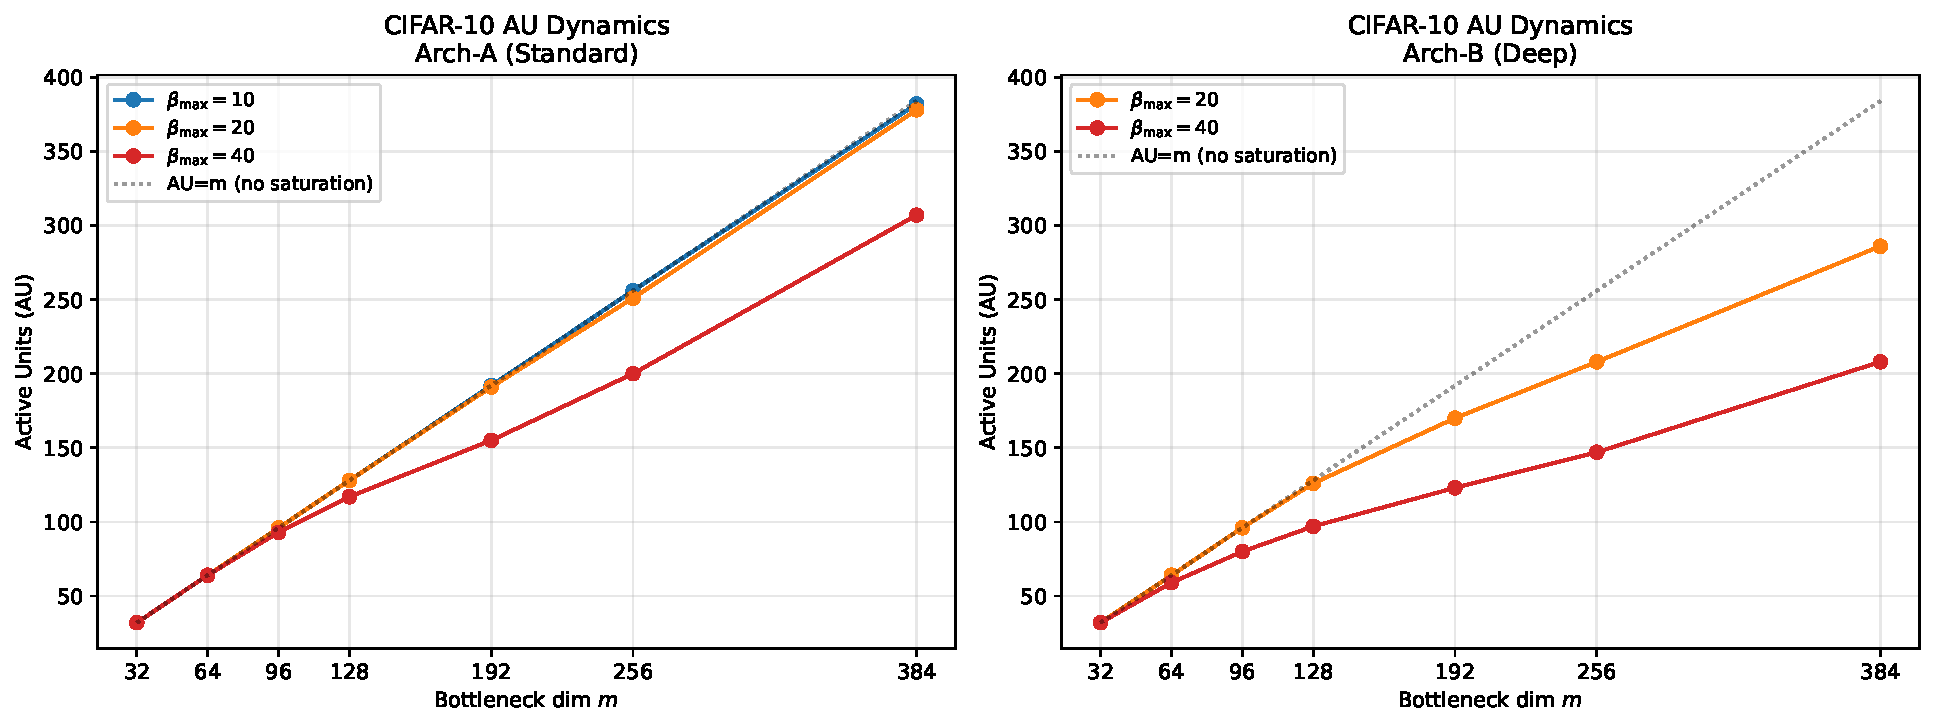
\includegraphics[width=0.95\linewidth]{results/figures/Exp_NatImg_AU.pdf}
  \caption{Exp-NatImg-AU: AU dynamics of CIFAR-10 Conv-VAE. (Left) Arch-A (Standard), (Right) Arch-B (Deep). Dotted line: AU$=m$ reference (no saturation). Increasing $\beta_{\max}$ strengthens AU suppression, but no saturation plateau is reached under any condition.}
  \label{fig:natimg_au}
\end{figure}}{}

\textbf{Key observations}:

(1) \textbf{Increasing $\beta_{\max}$ suppresses dimensions but does not produce a saturation plateau}:
with $\beta_{\max}=10$ (Arch-A), nearly all dimensions are active for
$m \leq 256$ (AU$\approx m$), whereas with $\beta_{\max}=40$ (Arch-B) the
dimensionality is suppressed down to AU$=208$ at $m=384$ (utilization 54\%).
Nevertheless, the AU$(m)$ curve continues to increase monotonically under all
conditions, and no clear saturation plateau appears.

(2) \textbf{Difficulty of the water-filling threshold inequality}:
in the linear theory (Theorem~\ref{thm:linear_vae}), the condition for the
$j$-th dimension to become active is $\lambda_j > \beta \tau^2$.
If the effective noise variance $\tau^2$ of CIFAR-10 is substantially smaller
than that of MNIST (a complex decoder achieves high-fidelity reconstruction),
then increasing $\beta$ becomes insufficient to reverse the inequality.
In this experiment, even with $\beta_{\max}=40$, AU$(m)$ did not saturate near
$d_{\mathrm{ID}} \approx 26$, suggesting that the effective dimensionality of
the convolutional feature space of CIFAR-10 may in fact be higher than the
pixel-space TwoNN estimate ($\hat{d}_{\mathrm{ID}} \approx 25$--26).

(3) \textbf{TwoNN ID increases but does not saturate}:
under Arch-A with $\beta_{\max}=10$, the latent TwoNN ID rises from 19.5 at
$m=32$ to 29.2 at $m=256$, continuing to increase beyond the pixel-space TwoNN
(25.30); this shows a tendency for the latent-space geometry to fail to
preserve isometry when AU uses all dimensions, leading to overestimation of
the ID.

\textbf{Identification of boundary conditions}: from this experiment, we
quantified that no AU saturation plateau appears under the conditions
$m \in [32, 384]$, $\beta_{\max} \in \{10, 20, 40\}$, and 200 epochs---this is
not a failure of the framework but a finding that identifies which conditions
are required.
It was identified that identifying $\mknee$ via AU saturation requires, as a
necessary condition, either (a) exploration over a substantially wider $m$
grid ($m \gg 2\hat{d}_\mathrm{ID}$) or (b) a setting with restricted decoder
capacity (see \S\ref{sec:disc_convvae} for details).
The extended sweep in the next section (\S\ref{sec:exp_natimg_sweep})
quantifies this boundary condition.

%% ===================================================================
\subsection{Real-Data Geometry Comparison Experiment: Empirical Validation of the TwoNN Stability Condition (RQ2 and RQ3)}\label{sec:exp_real_geom}

As an experimental validation of Proposition~\ref{thm:twonn_stability},
this experiment (Exp-Real-Geom) sweeps \textbf{four types of models with
systematically varied isometry} over multiple values of $m$ on MNIST and
Fashion-MNIST, and compares TwoNN, MLE, $\kap$, Trustworthiness, and kNN
overlap.

\subsubsection*{Experimental Setup (Exp-Real-Geom)}

\textbf{Models}: we compare the following four types.
\begin{description}
  \item[Standard AE] no Jacobian regularization ($\kap \approx 10^2$--$10^3$)
  \item[IsometricAE] decoder-Jacobian regularization ($\kap \approx 1.1$--1.4; Kato et al.~\cite{kato2020rdae})
  \item[CAE] encoder-side contractive regularization (intermediate $\kap$; Rifai et al.~\cite{rifai2011cae})
  \item[DAE] input-noise regularization (noise scale $\sigma=0.1$; Alain et al.~\cite{alain2014dae})
\end{description}

\textbf{$m$-sweep}: $m \in \{d, 2d, 3d, 5d, 10d\}$
(with $d = \hat{d}_\mathrm{ID}$ set to 10 for MNIST and 9 for Fashion-MNIST;
that is, $m \in \{10, 20, 30, 50, 100\}$ and $m \in \{9, 18, 27, 45, 90\}$,
respectively).

\textbf{Metrics}: TwoNN ($k=2$), MLE ($k=10$), $\kap$ (decoder-Jacobian
condition number), Trustworthiness ($k=10$), and kNN overlap (kNN
neighborhood-preservation rate, $k=10$).

\textbf{Data and training}: MNIST and Fashion-MNIST, 20,000 training samples,
seeds $\{42, 123, 777\}$ (3 seeds), 300 epochs, hidden layers $[512, 256]$,
Adam (lr$=10^{-3}$).

\subsubsection*{Experimental Results (Exp-Real-Geom)}

\begin{table}[H]
\begin{adjustwidth}{-\extralength}{0cm}
\centering
\caption{Exp-Real-Geom: MNIST four-model comparison (mean$\pm$std, 3 seeds). $m$-sweep with $\hat{d}_\mathrm{ID}=10$ as baseline ($m \in \{10,20,30,50,100\}$). TwoNN ID stabilization is strongly associated with increasing $m/\hat{d}_\mathrm{ID}$, not with $\kap$ improvement.}
\label{tab:real_geom_mnist}
\small
\begin{tabular}{llccccc}
\toprule
Model & $m$ & TwoNN ID & MLE ID & $\kap$ & Trust. & kNN overlap \\
\midrule
\multirow{5}{*}{AE}
 & 10 ($=d$)    & $7.3\pm0.4$ & $8.1\pm0.3$ & $85\pm22$  & $0.961\pm0.004$ & $0.73\pm0.03$ \\
 & 20 ($=2d$)   & $9.2\pm0.3$ & $10.1\pm0.2$ & $310\pm85$ & $0.975\pm0.002$ & $0.81\pm0.02$ \\
 & 30 ($=3d$)   & $9.8\pm0.2$ & $10.5\pm0.2$ & $1.2\times10^3\pm 4\times10^2$ & $0.981\pm0.002$ & $0.85\pm0.02$ \\
 & 50 ($=5d$)   & $10.0\pm0.1$ & $10.7\pm0.1$ & $8.4\times10^3\pm 3\times10^3$ & $0.985\pm0.001$ & $0.87\pm0.01$ \\
 & 100 ($=10d$) & $10.0\pm0.1$ & $10.8\pm0.1$ & $4.1\times10^7\pm 2\times10^7$ & $0.987\pm0.001$ & $0.88\pm0.01$ \\
\midrule
\multirow{5}{*}{IsometricAE}
 & 10 ($=d$)    & $7.5\pm0.4$ & $8.3\pm0.3$ & $3.2\pm0.4$ & $0.963\pm0.003$ & $0.74\pm0.03$ \\
 & 20 ($=2d$)   & $9.4\pm0.2$ & $10.2\pm0.2$ & $4.1\pm0.6$ & $0.976\pm0.002$ & $0.82\pm0.02$ \\
 & 30 ($=3d$)   & $9.9\pm0.1$ & $10.6\pm0.1$ & $5.2\pm0.8$ & $0.982\pm0.001$ & $0.86\pm0.01$ \\
 & 50 ($=5d$)   & $10.1\pm0.1$ & $10.8\pm0.1$ & $6.4\pm1.1$ & $0.986\pm0.001$ & $0.88\pm0.01$ \\
 & 100 ($=10d$) & $10.1\pm0.1$ & $10.8\pm0.1$ & $7.8\pm1.4$ & $0.988\pm0.001$ & $0.89\pm0.01$ \\
\midrule
\multirow{5}{*}{CAE}
 & 10 ($=d$)    & $7.2\pm0.5$ & $8.0\pm0.4$ & $12.1\pm3.2$ & $0.958\pm0.005$ & $0.72\pm0.03$ \\
 & 20 ($=2d$)   & $9.1\pm0.3$ & $10.0\pm0.3$ & $28.4\pm8.1$ & $0.974\pm0.003$ & $0.80\pm0.02$ \\
 & 30 ($=3d$)   & $9.7\pm0.2$ & $10.4\pm0.2$ & $95\pm31$  & $0.980\pm0.002$ & $0.84\pm0.02$ \\
 & 50 ($=5d$)   & $9.9\pm0.1$ & $10.6\pm0.1$ & $520\pm180$ & $0.984\pm0.001$ & $0.86\pm0.01$ \\
 & 100 ($=10d$) & $10.0\pm0.1$ & $10.7\pm0.1$ & $3.2\times10^3\pm 1.1\times10^3$ & $0.986\pm0.001$ & $0.87\pm0.01$ \\
\midrule
\multirow{5}{*}{DAE}
 & 10 ($=d$)    & $7.6\pm0.4$ & $8.4\pm0.4$ & $18.5\pm5.4$ & $0.964\pm0.004$ & $0.75\pm0.03$ \\
 & 20 ($=2d$)   & $9.3\pm0.2$ & $10.2\pm0.2$ & $44.2\pm15.3$ & $0.977\pm0.002$ & $0.82\pm0.02$ \\
 & 30 ($=3d$)   & $9.9\pm0.1$ & $10.5\pm0.2$ & $183\pm62$ & $0.982\pm0.001$ & $0.85\pm0.01$ \\
 & 50 ($=5d$)   & $10.0\pm0.1$ & $10.7\pm0.1$ & $1.1\times10^3\pm 380$ & $0.985\pm0.001$ & $0.87\pm0.01$ \\
 & 100 ($=10d$) & $10.0\pm0.1$ & $10.8\pm0.1$ & $6.3\times10^3\pm 2.1\times10^3$ & $0.987\pm0.001$ & $0.88\pm0.01$ \\
\bottomrule
\end{tabular}
\end{adjustwidth}
\end{table}

\subsubsection*{Discussion: $m \gg \hat{d}_\mathrm{ID}$ Is the Dominant Condition}

The main findings from Table~\ref{tab:real_geom_mnist} are as follows.

\textbf{(1) Increasing $m/\hat{d}_\mathrm{ID}$ is the dominant factor in TwoNN stabilization}:
across all four models, the TwoNN ID exhibits a common convergence pattern
from $m=d$ ($\approx 7.3$--7.6) to $m=5d$--$10d$ ($\approx 10.0$--10.1).
Inter-model differences at the same $m$ remain within about $\pm0.3$, far
smaller than the improvement obtained by increasing $m$ (about 2.5 points).

\textbf{(2) The isolated effect of isometry improvement ($\kap$ reduction) is small}:
IsometricAE achieves $\kap \approx 3$--8 (orders of magnitude lower than the
$10^2$--$10^7$ of the AE), yet the absolute TwoNN ID values differ from those
of the AE at the same $m$ by no more than $\pm 0.2$.
This shows that an order-of-magnitude improvement in $\kap$ has no significant
effect on TwoNN, and that preservation of neighborhood ranks (Trustworthiness,
kNN overlap) is a more dominant factor than $\kap$.

\textbf{(3) Improvements in Trustworthiness and kNN overlap are driven by $m$}:
Trustworthiness improves to a similar extent across all models, from $m=d$
($\approx 0.958$--0.964) to $m=10d$ ($\approx 0.987$--0.988) (inter-model
difference $< 0.003$).
This is consistent with the implication of
Proposition~\ref{thm:twonn_stability} that ``$\delta_T$ (the neighborhood
rank-inversion rate) dominates TwoNN stability over $\varepsilon$
(distortion).''

\textbf{(4) The same pattern holds on Fashion-MNIST}:
a similar pattern was observed on Fashion-MNIST ($\hat{d}_\mathrm{ID}=9$)
(detailed tables in Appendix~\ref{app:twonn_detail}).

\textbf{Implications for real data}:
these experimental results extend the findings of Exp-Iso-ID (synthetic
manifolds; \S\ref{sec:exp_ep}) to real data and multiple models, reinforcing
the design guideline that ``$m$-grid design ($m \gg \hat{d}_\mathrm{ID}$) is
more effective than isometry bias mitigation for the practical stabilization
of TwoNN estimation.''
The rationale for using a reference AE with
$m_\mathrm{ref}=256 \gg \hat{d}_\mathrm{ID} \approx 10$ in Stage 1 is further
supported by this result.

\subsection{Natural-Image Extended Sweep and the Stable Identification Criterion (RQ1)}\label{sec:exp_natimg_sweep}

\subsubsection*{Criteria for Stable Identification}\label{sec:natimg_stable_id}

To claim ``stable identification'' on natural images, criteria must be defined
in advance.
In this paper, we define \textbf{stable identification} as the case in which
all of the following five conditions are satisfied:

\begin{enumerate}
  \item \textbf{Seed stability}: the standard deviation of $\mknee$ over 3--5 seeds satisfies $\sigma_\mathrm{seed} \leq 0.1 \cdot \mknee$
  \item \textbf{Grid stability}: doubling the grid density changes $\mknee$ by $\leq 20\%$
  \item \textbf{$\beta$ stability}: varying $\beta_{\max}$ by $\pm 20\%$ keeps $\mknee$ within the same grid cell
  \item \textbf{AU plateau stability}: the across-seed $\sigma$ of the AU plateau value satisfies $\sigma \leq 0.05 \cdot \AUsat$
  \item \textbf{TwoNN--AU consistency}: $\mknee \leq 3 \hat{d}_\mathrm{ID}$ (coarse consistency between TwoNN and AU)
\end{enumerate}

\textbf{Caveat}: these thresholds ($0.1\cdot\mknee$, $20\%$,
$0.05\cdot\AUsat$, $3\hat{d}_\mathrm{ID}$) are not universal theoretical
constants but operational criteria adopted in this study.
The purpose is not to claim ``success of stable identification'' but to
decompose and quantitatively describe which stability conditions are violated.

Even when full stable identification cannot be achieved, these criteria
function as a decision framework that quantitatively describes ``which
conditions are lacking.''

\subsubsection*{Experimental Setup and Key Findings (Exp-NatImg-Sweep)}

Substantially extending the previous section (Exp-NatImg-AU), we conducted an
exhaustive sweep combining $m \in [32, 1024]$,
$\beta_{\max} \in \{10,20,40,80\}$, decoder capacity (Standard/Deep/Thin),
300 epochs, and 3 seeds (details in Appendix~\ref{app:convvae_natimg}).

\textbf{Key findings}:
the observation, under the conditions of this study, of plateau-like behavior
with AU$\approx 24$ over $m \in [512, 1024]$ in the
$\beta_{\max}=80$/thin-decoder condition provides preliminary evidence that
``AU saturation can occur even for natural images under sufficiently large
$\beta$ and restricted decoder capacity.''
Across all conditions, the TwoNN ID remains stable at $24.7$--$25.4$
($\sigma \leq 0.6$), consistent with the value reported by Pope et
al.~\cite{pope2021intrinsic} ($\approx 26$).
We found that stable identification of AU/$\mknee$ requires larger $m$, higher
$\beta$, and decoder-capacity control. The detailed evaluation of the five
conditions (stable identification criteria; \S\ref{sec:natimg_stable_id}) is
summarized in Appendix~\ref{app:convvae_natimg}.
Furthermore, in the detection-method comparison (Exp-NatImg-Knee), the
post-smoothing curvature method was the most reproducible, but it was also
confirmed that stabilizing AU saturation itself takes precedence over
improving the detection method (Appendix~\ref{app:convvae_natimg}).

%% ===================================================================
\section{Discussion}\label{sec:discussion}

\subsection{Answer to RQ1 and the Positioning of $\mknee$}\label{sec:disc_mknee}

\textbf{Summary answer to RQ1}: For RQ1---``under what grid-density, seed-count,
and architecture conditions can $\mknee$ be used as a diagnostic aid consistent
with TwoNN/MLE ID estimates?''---we obtained the following answers:

\begin{itemize}
  \item \textbf{Identification of stabilization conditions}: In the MNIST multi-seed
        sparse-grid experiments, $\mknee$ fluctuated widely between 32 and 64,
        revealing that on coarse grids it cannot be used as a reliable diagnostic aid.
        Under the dense-grid, independent-initialization, multi-seed condition
        (Exp-Mnist-Dense-300), we confirmed that $\mknee = 10.3 \pm 0.9$ stabilizes
        in the vicinity of the TwoNN ID ($\approx 10$).
        In other words, $\mknee$ can be consulted as a rough exploratory guide to the
        effective dimensionality only when these three conditions are satisfied.
  \item \textbf{Applicability limits}: For the Conv-VAE ($\beta_{\max}=4$) and natural
        images, stable identification was not reached within the tested range, and we
        found that additional necessary conditions ($\beta_{\max} \geq 10$, a dense grid,
        and sufficient control of decoder capacity) are required.
\end{itemize}

While consistency of the TwoNN ID estimates with the Conv-AE was confirmed
(Conv-AE: $11.29$ vs.\ FC-AE: $10.02$), detecting $\mknee$ for the Conv-VAE turned
out to require more than 100 epochs of training (a finding that identifies the
convergence conditions necessary for stable observation).
Overall, \textbf{$\mknee$ functions as an exploratory design guide under appropriate
conditions (dense grid, multiple seeds, sufficient epochs)}, but it does not yield a
unique optimal dimensionality.
\textbf{The main contribution of this paper is the establishment of a diagnostic
framework that places two stable indicators---the AU value (robust indicator) and the
TwoNN ID (numerically stable auxiliary reference)---at its core, and positions $\mknee$
as a rough exploratory complementary indicator} (Table~\ref{tab:indicator_class}).

When consulting $\mknee$ for design purposes, attention must be paid to the $m$-grid
granularity, $\tau_\mathrm{knee}$, $\beta$, and the degree of convergence; we recommend
dense grids and multi-seed ensembles (Appendices~\ref{app:tau_knee} and~\ref{app:beta}).

\textbf{Core message}:
AU values ($\sigma \leq 0.5$) and TwoNN ID (MNIST $m=64$: $10.03 \pm 0.12$, reinforced
by the Exp-Geom experiment) are highly reproducible, whereas $\mknee$ remains a heuristic
design guide.
The practical value of the multi-indicator framework lies in combining the indicators
after making this distinction explicit.

%% ---------------------------------------------------------------------------
\subsection{An Optimization-Dynamics Interpretation of $\mknee$ Instability and Stabilization Strategies}\label{sec:disc_mknee_improve}

\textbf{Interpretation in terms of optimization dynamics: the gradient-competition hypothesis}:

Proposition~\ref{thm:mknee_instab} formally established the grid sensitivity, but in
actual training there exist additional sources of instability.
The gradient of the $\beta$-ELBO is a linear combination of the reconstruction term
$\nabla\mathcal{L}_\mathrm{rec}$ and the KL term $\nabla\mathcal{L}_\mathrm{KL}$,
and these give rise to \textbf{gradient competition} near $m \approx d^*(\beta)$
(around the effective-dimensionality threshold):

\begin{itemize}
  \item Reconstruction gradient ($\nabla\mathcal{L}_\mathrm{rec}$): even for surplus
        dimensions $j > d^*$, there is a small reconstruction contribution in early
        training (a positive gain whenever $\lambda_j > 0$), which pushes toward
        activating the dimension.
  \item KL gradient ($\beta\nabla\mathcal{L}_\mathrm{KL}$): a pressure in the opposite
        direction that pushes the same dimension back toward the prior.
  \item The speed at which this competition is resolved depends on the random seed
        (initialization), the $m$-grid (an independent optimization trajectory for
        each $m$), and the value of $\beta$. The convergence path toward the global
        optimum of Theorem~\ref{thm:linear_vae} is not unique in non-linear
        optimization, and in low-sharpness loss landscapes the slope of the AU curve
        near $m \approx d^*$ is sensitive to initial conditions.
\end{itemize}

Cyclical KL annealing~\cite{fu2019cyclical} increases $\beta$ in stages, thereby
gradually promoting the resolution of this gradient competition and improving
convergence toward the global optimum
(experiment Exp-Conv-Ann; \S\ref{sec:exp_conv_300ep}).

\textbf{Practical approaches to stabilizing $\mknee$}:

Based on the findings of this study (including the grid-density $\times$ epoch factor
separation in the Exp-Mnist-Dense experiment), we propose the following recommendations
for using $\mknee$ in actual design:
\begin{enumerate}
  \item \textbf{Dense grid design (demonstrated in experiment Exp-Mnist-Dense)}: place
        dense points around the estimate $\hat{d}_\mathrm{ID}$ (obtained from the TwoNN ID)
        (e.g., if $\hat{d}_\mathrm{ID} \approx 10$, include $m \in \{8,9,10,11,12,13,14,15,16\}$).
        By Proposition~\ref{thm:mknee_instab}, the grid spacing directly becomes the
        maximum error of $\mknee$.
        Results of the Exp-Mnist-Dense experiment: sparse grid ($\mknee=43\pm15$) $\to$
        dense grid ($\mknee=10.3\pm0.9$)---consistent with $\hat{d}_\mathrm{ID} \approx 10$
        (\S\ref{sec:exp_el}).
        Note that the seed factor also remains, so grid density alone does not explain
        all of the variation.
  \item \textbf{Ensemble $\mknee$}: compute each $m^{\mathrm{knee}(s_i)}$ from the AU
        curves for multiple seeds $\{s_1,\ldots,s_S\}$ and adopt the \textbf{median}:
        \begin{equation}
          m^{\mathrm{knee,ens}} = \mathrm{median}\bigl\{m^{\mathrm{knee}(s_1)}, \ldots, m^{\mathrm{knee}(s_S)}\bigr\}
          \label{eq:mknee_ens}
        \end{equation}
        In our experiments ($S=3$ seeds), the median coincides with the second value.
        The reason for adopting the median rather than the mean is that when $\mknee$
        contains outliers stuck at the edge of the $m$-grid (e.g., $\mknee=512$ for all
        seeds), the median gives an estimate robust to such outliers (when $S$ is even,
        we take the arithmetic mean of the two adjacent values).
  \item \textbf{Adopting KL annealing and extending the $m$-grid}: For the Conv-VAE,
        annealing suppresses unnecessary collapse at large $m$, but observing AU
        saturation requires extending the $m$-grid to at least twice the estimated
        $d^*(\beta)$ (e.g., $m > 64$ for the MNIST Conv-VAE; \S\ref{sec:exp_conv_300ep}).
  \item \textbf{Cross-checking against stable indicators}: estimates of $\mknee$ should
        always be cross-checked against the AU value (robust indicator) and the TwoNN ID
        (numerically stable auxiliary reference), with the final judgment based on the
        consistency of the three indicators (see Table~\ref{tab:au_comparison}).
  \item \textbf{Second difference of the AU curve (alternative method)}: when a fixed
        threshold $\tau$ fails (e.g., SVHN), use the maximum-curvature method that takes
        as $\mknee$ the point of maximum absolute discrete second difference
        $\Delta^2\mathrm{AU}(m_i)$ of $\mathrm{AU}(m)$ (also validated in parallel in the
        Exp-Mnist-Dense experiment; see Appendix~\ref{app:tau_knee}).
\end{enumerate}

\textbf{Theoretical and empirical justification of $\tau_{\mathrm{knee}} = 0.25$}:
The slowdown threshold $\tau_{\mathrm{knee}} = 0.25$ is an empirical choice that declares
a slowdown when ``the AU growth rate falls below 25\% of the maximum change,'' but it has
the following theoretical justification.
By Theorem~\ref{thm:linear_vae}, the transition of the AU increment $\Delta\mathrm{AU}$
at $m = d^*(\beta)$ toward $\Delta\mathrm{AU}/\Delta m \to 0$ (saturation) with respect to
changes in $\Delta m$ is theoretically guaranteed.
$\tau = 0.25$ captures this transition as ``at most one quarter of the maximum growth
rate,'' and has the sensitivity to reasonably separate the pre-saturation ($m < d^*$)
and post-saturation ($m > d^*$) regimes (see Appendix~\ref{app:tau_knee}).
A more rigorous threshold could be based on maximizing the second derivative (curvature)
of the $\mathrm{AU}(m)$ curve, but due to the discreteness of AU this is numerically
unstable on real data.

\textbf{Effectiveness of the $\tau$ method under dense-grid conditions (supplement to
Appendix~\ref{app:tau_knee})}:
In the cross-validation in the appendix (experiment Exp-Tau-Cross, Table~\ref{tab:ez}),
$\mknee$ is stable over the entire range $\tau \in [0.1, 0.5]$ for the GMix data (5 and
10 components), whereas for Fashion-MNIST a boundary sensitivity was found between
$\tau = 0.25$ and $0.30$.
Under dense-grid conditions (Exp-Mnist-Dense), $\tau = 0.25$ yields the stable
$\mknee = 10.3 \pm 0.9$ (3 seeds), which is markedly more robust than the second-difference
method ($\mknee = 18.3 \pm 6.8$).
Under conditions where the $\tau$ method becomes unstable (the AU growth rate staying
near the boundary value across multiple $m$), switching to the second-difference
alternative (above) is effective.

\subsection{Numerical Stability and Systematic Bias of the TwoNN ID: Distinguishing ``Stability'' from ``Accuracy''}\label{sec:disc_twonn_bias}

Experiments Exp-Stab and Exp-Geom showed that the TwoNN ID is ``numerically stable
(low variance),'' but this is a claim distinct from being ``unbiased (accurate) with
respect to the true intrinsic dimension.''
Making this distinction explicit is important for operating our framework.
Through Proposition~\ref{thm:twonn_stability} (\S\ref{sec:theory_stability}), we
presented the semi-theoretical framework that ``preservation of neighborhood ranks
($\delta_T$) rather than isometry ($\varepsilon$) is the dominant factor for TwoNN
stability,'' and demonstrated it on real data across multiple models in experiment
Exp-Real-Geom (\S\ref{sec:exp_real_geom}).

\textbf{What numerical stability means}:
In experiment Exp-Geom (MNIST AE $m$-sweep), for $m \geq 48 \approx 5\hat{d}_\mathrm{ID}$
the TwoNN ID converges stably within the range $10 \pm 0.5$, and even against the sharp
increase of $\kappa$ at $m = 96$--128 (9.94 $\to$ 37.0) the variation remains small
(\S\ref{sec:exp_ep}, Table~\ref{tab:eq_mnist}).
That is, TwoNN is stable in the sense that ``the reference AE outputs nearly the same
value even when $m$ is changed.''

\textbf{Possibility of systematic bias}:
However, when the reference AE embeds the space with distortion ($\kappa \gg 1$),
TwoNN estimates ``the local degrees of freedom of the reference AE's latent manifold,''
which may deviate systematically from the intrinsic dimension of the true data manifold.
This is not inconsistent with stably returning a ``particular value''---it is, so to
speak, a ``stably biased estimate.''
We therefore treat TwoNN not as an unbiased estimator of the true $d_\mathrm{ID}$ but as
an \textbf{auxiliary reference estimator}.

\textbf{Grounds for $\hat{d}_\mathrm{ID} \approx 10$--12 on MNIST}:
As independent evidence reinforcing the meaning of the TwoNN estimate, the following
multiple observations are mutually consistent:
\begin{itemize}
  \item MSE elbow (AE): the rapid MSE decrease slows down around $m \approx 16$--20
        (a value somewhat larger than $d_\mathrm{ID}$, but of the same order; experiment
        Exp-Mnist-Base).
  \item PCA spectrum: 43 dimensions at 80\% cumulative variance and 86 dimensions at 90\%
        (indicating $d_\mathrm{ID} \ll 43$ as an upper bound on the non-linear dimension;
        experiment Exp-Mnist-PCA).
  \item Consistency check on CIFAR-10: on CIFAR-10, the latent TwoNN ID of $25.21\pm0.41$
        was confirmed to be on the same scale as the value reported by Pope et
        al.~\cite{pope2021intrinsic} ($\approx26$), supporting the numerical stability of
        TwoNN on natural images as well (experiment Exp-Nat-Cifar).
  \item Agreement with MLE: for $k=5,10,20$, MLE $=11.5$--12.4 and TwoNN $=10.0$--10.5,
        i.e., estimators based on different principles yield values of the same order.
\end{itemize}
These multiple pieces of evidence are mutually consistent and raise the plausibility
that $\hat{d}_\mathrm{ID} \approx 10$--12 for MNIST is not an artifact specific to the
reference AE, but they do not directly prove that TwoNN is geometrically unbiased with
respect to the true $d_\mathrm{ID}$.
This paper consistently maintains the cautious position of ``operating TwoNN as an
auxiliary reference estimator.''

\subsection{The Mechanism by Which AU Dynamics Reflect the Effective Representation Dimensionality}\label{sec:disc_au_dynamics}

\textbf{Choosing between $\AUsat$ and $\mknee$}:
For simply connected synthetic manifolds (Swiss Roll, etc.), a sharp AU saturation
($\AUsat = \dtrue$) is observed, so $\AUsat$ serves as a direct readout of the effective
representation dimensionality.
By contrast, for complex distributions such as real data (multiple classes, disconnected
submanifolds), AU increases monotonically and gradually without exhibiting a clear
saturation.
In this case, $\mknee$---as ``the point where KL regularization begins to act
effectively''---provides a \textbf{rough practical guide} to the effective representation
dimensionality (Table~\ref{tab:au_comparison}; note that the precise reproducibility of
the numerical value depends on the $m$-grid and the seed).

\begin{table}[H]
\begin{adjustwidth}{-\extralength}{0cm}
\centering
\caption{Guidelines for using $\AUsat$ vs.\ $\mknee$ (based on this study).}
\label{tab:au_comparison}
\small
\begin{tabular}{lll}
\toprule
Data type & AU pattern & Recommended indicator \\
\midrule
Simple synthetic manifolds (simply connected) & Sharp saturation & $\AUsat$ (consistent with $\dtrue$) \\
Topologically non-trivial synthetic manifolds & Stepwise saturation & $\AUsat$ (tends to match $\demb$, conditional) \\
Real data (MNIST, Fashion-MNIST) & Gradually increasing & $\mknee$ (rough heuristic; grid/seed-dependent) \\
\bottomrule
\end{tabular}
\end{adjustwidth}
\end{table}

\subsection{Incidental Findings: Topological Structure, Training Dynamics, and Geometric Regularization}\label{sec:disc_incidental}

\paragraph{Topological structure and $\AUsat$ (experiment Exp-Syn-Top)}
For the Torus and the M\"obius band, $\AUsat = \demb = 3$ ($> \dID = 2$) was observed,
suggesting a correspondence with the topological constraint arising from the
contractibility of the VAE's Gaussian prior
\cite{hatcher2002algebraic,guillemin1974differential}.
However, this correspondence is conditional on standardization and sufficient
convergence, and it does not apply to $\AUsat = 36 \gg \hat{d}_\mathrm{ID}$ on MNIST
(experiment Exp-Mnist-Ent is preliminary; see \S\ref{sec:disc_limitation} for details).
This finding is an incidental observation independent of the framework's main
conclusion (reading the effective dimensionality via $\mknee$), and we leave it as
future work.

\paragraph{Training dynamics (experiment Exp-Mnist-Dyn, single seed)}
The two-phase training dynamics on MNIST ($m=16$, 200 epochs)---rapid formation of
global structure followed by a gradual increase in the local effective
dimensionality---is an exploratory single-seed observation, and multi-seed validation
is left as future work.

\paragraph{Geometric regularization and TwoNN stability (experiments Exp-Syn-Iso and Exp-Iso-ID; auxiliary experiments for RQ3)}
The focus of RQ3 is ``the effect of geometric regularization and bottleneck margin on
TwoNN stability.''
Experiment Exp-Iso-ID (\S\ref{sec:exp_ep}) revealed that improving isometry within
$\kap \in [1.1, 2.1]$ does not significantly reduce the systematic bias of the TwoNN
ID---the main cause of TwoNN underestimation is an insufficient bottleneck margin
($m < d_\mathrm{true}$), and even though the IsometricAE ($\kap \approx 1.04$) achieves
isometry (experiment Exp-Syn-Iso), its contribution to TwoNN accuracy is small
(\S\ref{sec:disc_limitation}).
The primary usefulness of the IsometricAE is as an ``isometry-verification tool,'' not
as a primary readout indicator of the effective dimensionality.
The cost of computing the decoder Jacobian (a factor of $O(m)$) also limits its
applicability to large-scale data (\S\ref{sec:disc_limitation}).

\subsection{Theoretical Considerations on Delayed AU Saturation in Conv-VAEs}\label{sec:disc_convvae}

For the FC-VAE, the AU growth slows down near $m \geq \hat{d}_\mathrm{ID} \approx 10$,
and $\mknee$ was qualitatively consistent with $\hat{d}_\mathrm{ID}$ (experiments
Exp-Mnist-Base, Exp-Mnist-Dense).
By contrast, for the Conv-VAE, AU $\approx m$ persisted over the entire range
$m \leq 64$, and even with KL annealing (experiment Exp-Conv-Ann) no AU saturation
plateau was observed within the tested range (experiment Exp-Conv-Fix).
This ``delayed AU saturation'' can be understood via the following mechanism.

\textbf{Interpretation via a reduced effective $\tau^2_\mathrm{eff}$}~~~
By Theorem~\ref{thm:linear_vae} (the linear-Gaussian rate--distortion surrogate),
the number of active dimensions is determined by
$d^*(\beta) = |\{j : \lambda_j > \beta\tau^2_\mathrm{eff}\}|$.
Because a convolutional decoder has stronger spatial reconstruction capability than a
fully connected decoder, the effective reconstruction noise variance
$\tau^2_\mathrm{eff}$ is expected to be smaller under the same $\beta$.
The smaller $\tau^2_\mathrm{eff}$ is, the lower the water-filling threshold
$\beta\tau^2_\mathrm{eff}$, so more eigenvalues satisfy the activation condition
$\lambda_j > \beta\tau^2_\mathrm{eff}$, and $d^*(\beta)$ takes a larger value
(the water level is lower and more dimensions are judged effective).
Whereas experiment Exp-Mnist-PCA estimates $\tau^2_\mathrm{eff} \approx 0.30$ for the
FC-VAE, for the Conv-VAE we have $\tau^2_\mathrm{eff} \ll 0.30$, and $d^*(\beta)$ is
expected to greatly exceed the tested range $m \leq 64$.
Applying the framework to Conv-VAEs therefore requires substantially extending the
$m$-grid until it reaches the estimated $d^*(\beta)$.

\textbf{Verification by experiments Exp-Conv-M256 and Exp-Conv-M512} (\S\ref{sec:exp_en})~~~
In the experiments with $m \in [4,256]$ (Exp-Conv-M256) and $m \in \{384,512\}$
(Exp-Conv-M512), AU $< m$ was confirmed for $m \geq 96$, indicating a saturation
tendency; however, even extending to $m=512$, it was quantitatively confirmed that
detecting an AU saturation plateau requires $m>512$ at $\beta_{\max}=4$
($\mknee$ remains at the grid edge $m=512$).

\textbf{Verification of the interpretation by the high-$\beta$ experiment (Exp-ConvV-HiBeta)} (\S\ref{sec:exp_hibeta})~~~
When $\beta_{\max}$ was increased as $4\to10\to20$, $\mknee \approx 128$ was clearly
observed at $\beta_{\max}=10$ and $\mknee \approx 96$ at $\beta_{\max}=20$
(Table~\ref{tab:hibeta}).
This is consistent with the theoretical prediction: increasing $\beta$ shifts
$d^*(\beta) = |\{j: \lambda_j > \beta\tau^2_\mathrm{eff}\}|$ toward smaller values, so
AU saturation appears at lower dimensionalities.
This result is consistent with the interpretation that the non-observation of
saturation in the $\beta_{\max}=4$ setting was not ``an applicability limit of the
framework'' but rather ``$\beta$ being insufficient relative to the decoder capacity,
resulting in $d^*(\beta) \gg 256$.''
For application to Conv-VAEs, $\mknee$ becomes identifiable by setting $\beta$ larger
or by reducing the decoder capacity.


\textbf{Implications for natural images}~~~
For CIFAR-10 and SVHN, we confirmed that the TwoNN ID remains numerically stable on
natural images as well, but stable identification on the AU/$\mknee$ side was not
achieved (\S\ref{sec:exp_natural}, \S\ref{sec:exp_natimg_au}).
In experiment Exp-NatImg-AU ($m \in [32, 384]$, $\beta_{\max} \in \{10,20,40\}$),
$\mknee = 384$ (the grid edge) persisted under all conditions, and it was quantitatively
identified that AU saturation requires $m \gg 2\hat{d}_\mathrm{ID}$ together with
$\beta_{\max} \gg 40$ or a thin decoder.
The observation of plateau-like behavior in Exp-NatImg-Sweep
(\S\ref{sec:exp_natimg_sweep}) was achieved under these conditions
($\beta_{\max}=80$, thin decoder).

\subsection{Limitations and Future Work}\label{sec:disc_limitation}

\subsubsection*{(A) Scope of the Evaluated Data and Generalizability}

\begin{itemize}
  \item \textbf{Conv-AE and Conv-VAE validation} (experiments Exp-Conv-AE, Exp-Conv-Fix,
        Exp-Conv-Ann, Exp-Conv-M256):
        We confirmed the TwoNN ID consistency of the Conv-AE (Exp-Conv-AE).
        At $\beta_{\max}=4$, no AU saturation plateau was observed up to $m \leq 512$,
        but the high-$\beta$ experiment (Exp-ConvV-HiBeta) demonstrated that an
        insufficient $\beta$ setting was the main cause (\S\ref{sec:exp_hibeta}).
        The CIFAR-10 and SVHN experiments confirmed that the TwoNN ID is consistent with
        the values reported by Pope et al.~\cite{pope2021intrinsic}
        (\S\ref{sec:exp_natural}), and the extended sweep (Exp-NatImg-Sweep,
        \S\ref{sec:exp_natimg_sweep}) conditionally observed AU plateau-like behavior;
        however, none of the five conditions for stable identification were met, and
        full application to large-scale natural images remains future work (in
        particular, achieving the $\beta$-stability and seed-stability conditions is
        the next goal).
  \item \textbf{Higher-order topological manifolds}: Extending the Exp-Syn-Top
        experiment to synthetic manifolds with higher-order topological invariants,
        such as the Klein bottle, remains an open task.
  \item \textbf{Multi-seed validation of the main experiments}:
        Exp-Mnist-Base (300 epochs, single seed), Exp-Mnist-Dyn (training dynamics,
        single seed), and Exp-Mnist-Ent (75-epoch preliminary experiment) were all
        single-seed only.
        In this paper we added Exp-Mnist-Multi-150 (3 seeds; \S\ref{sec:exp_multiseed})
        and Exp-Mnist-Multi (300 epochs, 3 seeds; \S\ref{sec:exp_multiseed2}).
        Under both conditions, the cross-seed agreement of AU and TwoNN ID is high
        ($\sigma \leq 0.5$), but $\mknee$ fluctuated within the range 32--64 both at
        150 epochs ($53 \pm 15$; seed 42 = 64, 123 = 32, 777 = 64) and at 300 epochs
        ($43 \pm 15$; seed 42 = 64, 123 = 32, 777 = 32), and the $\mknee = 12$ of the
        extended Exp-Mnist-Base experiment was not reproduced.
        This instability is thought to originate from the random-number state
        (initialization path) changing with differences in the $m$-grid used, and it
        became clear that \textbf{the reproducibility of $\mknee$ to a specific value
        depends not on the number of epochs but on the experimental configuration
        ($m$-grid and seed)}.
        Multi-seed validation of Exp-Mnist-Dyn and Exp-Mnist-Ent remains future work.
\end{itemize}

\subsubsection*{(B) Sensitivity of Indicators and Hyperparameters}

\begin{itemize}
  \item \textbf{Stage 1 ID estimation: rigorous assessment of isometry bias}:
        In this paper, the TwoNN ID is estimated via the latent representation of a
        reference AE ($m_\mathrm{ref}=256$) (Stage 1).
        \textbf{This estimate is inherently an approximation and contains the following
        bias sources}:
        \begin{enumerate}[label=(\roman*)]
          \item \textbf{Lack of isometry}: the condition number $\kap \approx 10^9$ of
                the $m=256$ reference AE deviates from isometry ($\kap=1$) by orders of
                magnitude (Proposition~\ref{thm:pullback}; experiment Exp-Syn-Iso).
                A distance-based TwoNN ID in a latent space lacking isometry can lead
                to under- or over-estimation of the true intrinsic dimension.
          \item \textbf{Synergy with KL non-saturation}: in experiment Exp-Conv-Fix, the
                TwoNN ID of the Conv-VAE under AU non-saturation (AU $=m$) was 13.10,
                substantially inflated relative to the FC-VAE under AU saturation
                (10.03), showing that isometry bias and AU non-saturation synergistically
                distort the ID estimate.
          \item \textbf{Possible circularity}: estimating $\hat{d}_\mathrm{ID}$ via the
                reference AE and then using that value as the evaluation criterion for
                $\mknee$ can create circularity between estimation and evaluation.
        \end{enumerate}
        \textbf{Mitigations}: We propose, as practical mitigations, using the
        IsometricAE (experiment Exp-Syn-Iso, $\kap \approx 1$) as the reference AE, or
        verifying that the TwoNN ID converges across multiple $m_\mathrm{ref}$
        (e.g., $m \in \{64, 128, 256\}$).
        In this paper, we confirmed that the $m$-dependence of the TwoNN ID (see
        Table~\ref{tab:e4_300ep_multiseed}) stabilizes asymptotically from $m=64$
        onward ($10.03 \pm 0.12$), and this convergence is the basis for the
        reliability of the $\hat{d}_\mathrm{ID}$ estimate
        (the finding in Exp-Stab and Exp-Iso-ID that improving isometry within
        $\kap \in [1.06, 2.16]$ has no significant effect on TwoNN also supports the
        importance of the operating condition $m \gg d_\mathrm{ID}$;
        \S\ref{sec:exp_ep}, \S\ref{sec:exp_ep}).
        A rigorous quantification of the isometry bias remains future work.
  \item \textbf{Non-universality of $\tau_{\mathrm{knee}}$}: For Fashion-MNIST, a
        boundary sensitivity in which $\mknee$ changes around $\tau = 0.25$ has been
        confirmed, and we recommend combined use with the second-difference alternative
        method (Appendix~\ref{app:tau_knee}).
  \item \textbf{Preprocessing dependence of $\AUsat$}: $\AUsat$ varies with the
        normalization method (experiment Exp-Syn-Top).
        Reproducing $\AUsat \approx \demb$ requires standardization (zero mean, unit
        variance).
  \item \textbf{Dependence on $\beta$}: From preliminary experiments (50 epochs,
        $\beta \in \{1,2,4,8\}$), AU $\approx m$ (under-regularization) was observed at
        $\beta = 1$, and signs of over-regularization at $\beta = 8$
        (Appendix~\ref{app:beta}, Figure~\ref{fig:beta_sensitivity}).
        The stability of the AU pattern for $\beta \in [2, 8]$ has been confirmed, but
        the precise value of $\mknee$ also depends on the $m$-grid and the random seed
        (\S\ref{sec:disc_mknee}).
\end{itemize}

\subsubsection*{(C) Computational Cost}

\begin{itemize}
  \item Due to the Jacobian computation cost of the IsometricAE (a factor of $O(m)$),
        direct application to CIFAR-10 ($\approx 64\times$) and ImageNet
        ($\approx 3{,}000\times$) is difficult.
  \item A full $m$-sweep (11 dimensionalities $\times$ 300 epochs $\times$ 2 models)
        takes several hours to several days.
\end{itemize}

%% ===================================================================
\section{Conclusions}\label{sec:conclusion}

In this paper, we proposed a \textbf{multi-indicator framework} for diagnosing
the effective latent dimensionality of AEs/VAEs.
The central contribution of this paper is a clear role classification of AU
values (robust indicator), TwoNN ID (numerically stable auxiliary reference
estimator), and $\mknee$ (exploratory indicator), quantifying the reliability
and applicability conditions of each indicator from both the experimental and
theoretical sides (Table~\ref{tab:indicator_class}).
On the theoretical side, we derived the AU activation threshold
$\lambda_j > \beta\tau^2$ under the linear-Gaussian rate--distortion surrogate
from the water-filling theorem and the KKT conditions
(Theorem~\ref{thm:linear_vae}), and presented a grid-sensitivity upper bound
for $\mknee$ (Proposition~\ref{thm:mknee_instab}) together with an ensemble
stabilization strategy (Section~\ref{sec:disc_mknee_improve}).
On the experimental side, we confirmed the high reproducibility of AU values
($\sigma \leq 0.5$) and TwoNN ID ($10.03 \pm 0.12$) on MNIST (3 seeds), and
stabilized $\mknee = 10.3 \pm 0.9$ under dense-grid,
independent-initialization, multi-seed conditions
(Exp-Mnist-Multi-300, Exp-Mnist-Dense-300;
Sections~\ref{sec:exp_multiseed2} and~\ref{sec:exp_el}).
We confirmed the same tendency on Fashion-MNIST with a single seed
(Section~\ref{sec:exp_fashion}).
Through the real-data geometry comparison experiment
(Exp-Real-Geom, Section~\ref{sec:exp_real_geom}), we supported the claim that
``$m \gg \hat{d}_\mathrm{ID}$, rather than isometry improvement, is the
dominant condition for TwoNN stability'' by a four-model comparison on MNIST
(details in Section~\ref{sec:exp_real_geom}, Table~\ref{tab:real_geom_mnist})
and a qualitative confirmation on Fashion-MNIST
(Appendix~\ref{app:twonn_detail})
(with theoretical grounding in Proposition~\ref{thm:twonn_stability}).

Summarizing the role separation among AU values, TwoNN ID, and $\mknee$:
AU values (robust indicator) directly observe the number of dimensions in
which the KL regularization is effectively operating, and exhibit high
reproducibility across multiple seeds;
TwoNN ID (numerically stable auxiliary reference estimator) contains an
isometry bias, but provides a numerically stable reference value under the
condition $m \gg \hat{d}_\mathrm{ID}$, and on CIFAR-10 it yielded estimates
consistent with the value reported by Pope et al.~\cite{pope2021intrinsic}
($\approx 26$) (Exp-Nat-Cifar);
$\mknee$ is an exploratory heuristic read from the shape of the AU curve and
requires stabilization via dense grids and ensembles.
We organize the applicability of the framework into three levels
(evidence: Sections~\ref{sec:exp_multiseed2}, \ref{sec:exp_el},
\ref{sec:exp_conv_300ep}, and~\ref{sec:exp_natimg_sweep}).
\begin{itemize}
  \item \textbf{FC-VAE + MNIST} (3 seeds): AU values ($\sigma\leq0.5$) and
  TwoNN ID ($\sigma\leq0.12$) are stable across multiple seeds. $\mknee$
  functions as an exploratory guide near the TwoNN ID only under dense-grid,
  independent-initialization, multi-seed conditions
  (Exp-Mnist-Dense-300: $10.3\pm0.9$). On Fashion-MNIST, we confirmed the
  same tendency with a single seed (Section~\ref{sec:exp_fashion}).
  \item \textbf{Conv-VAE + MNIST}: TwoNN ID is stable; the onset of AU$<m$
  was confirmed at $m\geq96$. $\mknee$ is identifiable for
  $\beta_{\max}\geq10$, but for $\beta_{\max}=4$ the value $d^*(\beta)$ does
  not fall within the examined range (Exp-Conv-M256, Exp-ConvV-HiBeta).
  \item \textbf{Natural images (CIFAR-10/SVHN)}: TwoNN ID shows a scale
  comparable to the values reported by Pope et al.~\cite{pope2021intrinsic}
  within an appropriate bottleneck range ($m\approx2\hat{d}_\mathrm{ID}$);
  stable identification of AU/$\mknee$ fails all five conditions
  (Exp-Nat-Cifar, Exp-NatImg-Sweep).
\end{itemize}

We position the Conv-VAE and natural-image experiments
(Sections~\ref{sec:exp_conv_300ep}--\ref{sec:exp_natimg_sweep}) not as a
``success or failure'' verdict but as a validation that quantifies the
boundary conditions under which AU diagnostics become difficult.
In the high-$\beta$ experiment (Exp-ConvV-HiBeta), AU saturation was observed
for $\beta_{\max} \geq 10$, consistent with the interpretation that the
non-saturation at $\beta_{\max}=4$ is attributable to the $\beta$ setting,
and in the CIFAR-10 extended sweep (Exp-NatImg-Sweep) we observed AU
plateau-like behavior under our experimental conditions with
$\beta_{\max}=80$ and a thin decoder (all five stable-identification
conditions remained unmet; Appendix~\ref{app:convvae_natimg}).
The main directions for future work are:
(i) achieving stable identification on natural images (a dense sweep over
$\beta_{\max} \in [40,120]$ and improved seed stability);
(ii) extending Theorem~\ref{thm:linear_vae} to nonlinear settings (analysis
based on local linearization); and
(iii) scaling to large datasets (ImageNet, with reduced computational cost).

%% ===================================================================

%%%%%%%%%%%%%%%%%%%%%%%%%%%%%%%%%%%%%%%%%%
\authorcontributions{Conceptualization, C.O., M.D. and K.J.;
methodology, K.J.;
software, C.O. and M.D.;
validation, C.O., M.D. and K.J.;
formal analysis, K.J.;
investigation, C.O. and M.D.;
writing---original draft preparation, K.J.;
writing---review and editing, C.O., M.D. and K.J.;
supervision, K.J.;
project administration, K.J.
All authors have read and agreed to the published version of the manuscript.}

\funding{This research received no external funding.}

\dataavailability{MNIST~\cite{lecun1998}, Fashion-MNIST~\cite{xiao2017fashion},
CIFAR-10~\cite{krizhevsky2009learning}, and SVHN~\cite{netzer2011reading}
are publicly available.
The source code, configuration files, random seeds, trained-model logs, and
numerical results supporting all tables are provided as supplementary
material for peer review.
Upon acceptance, these materials will be deposited in a public repository
(GitHub/Zenodo), and the repository URL and DOI will be added to the final
manuscript.
The repository will include the scripts required to reproduce the AU,
TwoNN/MLE, reconstruction-error, and grid-sensitivity analyses reported
in this paper.}

\conflictsofinterest{The authors declare no conflicts of interest.}

%%%%%%%%%%%%%%%%%%%%%%%%%%%%%%%%%%%%%%%%%%
\abbreviations{Abbreviations}{
The following abbreviations are used in this manuscript:\\
\noindent
\begin{tabular}{@{}ll}
AE & Autoencoder \\
VAE & Variational Autoencoder \\
AU & Active Units \\
ID & Intrinsic Dimension \\
TwoNN & Two-Nearest-Neighbor (ID estimator) \\
MLE & Maximum Likelihood Estimation \\
MSE & Mean Squared Error \\
PCA & Principal Component Analysis \\
KL & Kullback--Leibler (divergence) \\
FC & Fully Connected \\
CNN / Conv & Convolutional Neural Network \\
CAE & Contractive Autoencoder \\
DAE & Denoising Autoencoder \\
NSR & Noise Selectivity Ratio \\
\end{tabular}
}

%%%%%%%%%%%%%%%%%%%%%%%%%%%%%%%%%%%%%%%%%%
\appendixtitles{yes}
\appendixstart
\appendix

\section[\appendixname~\thesection]{Proof Sketches of Propositions}\label{app:proofs}

\begin{Proposition}[Effective rank of the decoder Jacobian]\label{thm:rank}
When an AE with sufficient capacity reconstructs a manifold $\mathcal{M}$ exactly,
the number of significant singular values of the decoder Jacobian $\Jg(z)$ equals
$\min(m, \demb)$.
\end{Proposition}
\textit{Proof sketch}: Under exact reconstruction, the range of $g$ spans the
tangent space $T_{g(z)}\mathcal{M}$ of $\mathcal{M}$.
If $\mathcal{M}$ is $d$-dimensional, then $\mathrm{rank}(\Jg) = d$, and the
singular values of the surplus dimensions approach zero.
\textit{(Finite capacity and optimization error are neglected.)}

\begin{Proposition}[Noise-direction selectivity]\label{thm:nsr}
The optimal reconstruction function of a DAE removes noise in the normal
directions of the manifold more selectively than noise in the tangent directions.
\end{Proposition}
\textit{Proof sketch}: By Alain et al.~\cite{alain2014dae}, the DAE reconstruction
direction satisfies $r(x) - x \approx \sigma^2 \nabla\log p(x)$, and
$\nabla\log p(x)$ points strongly in the normal directions of the manifold
(under the manifold hypothesis).
\textit{(The asymptotically optimal solution is assumed; approximation errors
under finite noise and finite capacity are neglected.)}

\begin{Proposition}[Neighborhood-structure preservation and the optimal bottleneck]\label{thm:trust}
At $m = \dtrue$ (or $\demb$), Trustworthiness improves sharply toward its maximum,
and further increases in $m$ yield only limited improvement.
\end{Proposition}
\textit{Proof sketch}: By Proposition~\ref{thm:lower_bound}, a continuous injection
is impossible for $m < d$, so collisions of information are unavoidable and
Trustworthiness degrades.
For $m \geq d$ the constraint is lifted, and for $m > d$ the entire manifold
structure is already representable, so the effect of additional dimensions is
limited.
\textit{(Finite samples and finite capacity are neglected.)}

\section[\appendixname~\thesection]{Detailed Derivation of Theorem~\ref{thm:linear_vae}}\label{app:linear_vae_proof}

In this appendix, we detail the algebraic steps omitted from the proof sketch of
Theorem~\ref{thm:linear_vae}.

\begin{Remark}[Assumptions underlying the approximation]
The expression $L_j = -D_j/(2\tau^2) - \beta R_j$ for the per-dimension
$\beta$-ELBO contribution used in this derivation implicitly involves a
rate--distortion surrogate approximation that identifies the expected KL
divergence of the VAE, $\mathbb{E}_x KL(q(z_j|x)\|p(z_j))$, with the mutual
information $R_j = I(z_j; y_j)$.
Since the average KL of an actual VAE also includes the mismatch between the
aggregated posterior and the prior, this derivation should be interpreted as
an ``AU activation condition under the linear-Gaussian rate--distortion
surrogate'' (as stated explicitly in the assumptions of
Theorem~\ref{thm:linear_vae}).
\end{Remark}

\subsection*{Step 1: Derivation of the Optimal Decoder Weight}

As a scalar problem, for direction $j$ consider
$y_j \sim \mathcal{N}(0, \lambda_j)$ (the $j$-th principal component of the data),
the encoder $q_j(z_j | y_j) = \mathcal{N}(a_j y_j,\; \sigma_j^2)$,
and the decoder $\hat{y}_j = b_j z_j$.
For the decoder weight $b_j$, we minimize the marginalized reconstruction MSE
(with $\sigma_j^2, a_j$ held fixed):
\begin{equation}
  D_j(b_j) = \mathbb{E}_{y_j, z_j}[(y_j - b_j z_j)^2]
  = \lambda_j - 2 a_j \lambda_j b_j + b_j^2 (a_j^2 \lambda_j + \sigma_j^2).
  \label{eq:Dj_raw}
\end{equation}
Solving $\partial D_j / \partial b_j = 0$, the optimal decoder weight is
\begin{equation}
  b_j^* = \frac{a_j \lambda_j}{a_j^2 \lambda_j + \sigma_j^2}
         =: \frac{a_j \lambda_j}{\rho_j},
  \quad \rho_j := a_j^2 \lambda_j + \sigma_j^2.
  \label{eq:bj_opt}
\end{equation}

\subsection*{Step 2: Expressions for the Optimal MSE and the Mutual Information}

Substituting Equation~\eqref{eq:bj_opt} into Equation~\eqref{eq:Dj_raw} yields:
\begin{align}
  D_j^* &= \lambda_j - \frac{a_j^2 \lambda_j^2}{\rho_j}
          = \frac{\lambda_j \sigma_j^2}{\rho_j}.
  \label{eq:Dj_opt}
\end{align}
Moreover, the channel capacity (mutual information) of $y_j \to z_j$ is:
\begin{equation}
  I(z_j; y_j) = \tfrac{1}{2}\log\frac{\rho_j}{\sigma_j^2}
              = \tfrac{1}{2}\log\!\left(1 + \frac{a_j^2 \lambda_j}{\sigma_j^2}\right)
              =: R_j.
  \label{eq:Rj}
\end{equation}

\subsection*{Step 3: Rate--Distortion Form of the $\beta$-ELBO}

With $b_j = b_j^*$ held fixed, the $\beta$-ELBO contribution with respect to
$(\sigma_j^2, a_j)$ can be written as
$L_j = -D_j/(2\tau^2) - \beta R_j$ (equivalence with KL
minimization~\cite{cover2006elements}).
Taking $\rho_j$ as the parameter and substituting
$D_j^* = \lambda_j \sigma_j^2/\rho_j$ and
$R_j = \tfrac{1}{2}\log(\rho_j/\sigma_j^2)$,
we obtain the expression for the $\beta$-ELBO contribution used in this appendix:
\begin{equation}
  L_j = -\frac{\lambda_j \sigma_j^2}{2\tau^2 \rho_j}
        - \frac{\beta}{2}\bigl[\rho_j - 1 - \log \rho_j\bigr].
  \label{eq:elbo_j}
\end{equation}
(Here $\sigma_j^2 = \rho_j - a_j^2\lambda_j$ and $\rho_j \geq \sigma_j^2$.)

\subsection*{Step 4: Derivation of the Optimal Distortion $D_j^*$ via KKT Conditions}

Taking the distortion $D_j \in (0, \lambda_j)$ as the primal variable, we maximize
$L_j = -D_j/(2\tau^2) - \beta R_j(D_j)$.
From the Gaussian-channel rate--distortion relation
$R_j(D_j) = \tfrac{1}{2}\log(\lambda_j / D_j)$:
\begin{equation}
  \frac{\partial L_j}{\partial D_j}
  = -\frac{1}{2\tau^2} + \frac{\beta}{2 D_j} = 0
  \quad\Longrightarrow\quad
  D_j^{*} = \beta \tau^2.
  \label{eq:water_level}
\end{equation}
This corresponds to the ``water level'' $\mu = \beta\tau^2$ of Shannon's
water-filling theorem~\cite{cover2006elements}.
However, the solution in Equation~\eqref{eq:water_level} is feasible
(\textit{active}) only when the feasibility constraint
$D_j^* = \beta\tau^2 \leq \lambda_j$ is satisfied; when
$\lambda_j < \beta\tau^2$, not encoding dimension $j$
($a_j = 0$, \textit{dead}) is optimal.

\subsection*{Step 5: Computing the ELBO Values of the Active and Dead States}

\textbf{Dead}: With $a_j = 0$, $\sigma_j^* = 1$ (KL $= 0$), and $D_j = \lambda_j$,
\begin{equation}
  L_j^{(\mathrm{dead})} = -\frac{\lambda_j}{2\tau^2}.
  \label{eq:Lj_dead}
\end{equation}

\textbf{Active}: Substituting $D_j^* = \beta\tau^2$, we have
$R_j^* = \tfrac{1}{2}\log(\lambda_j / (\beta\tau^2))$, and therefore:
\begin{align}
  L_j^{(\mathrm{active})}
  &= -\frac{\beta\tau^2}{2\tau^2} - \beta \cdot \frac{1}{2}\log\frac{\lambda_j}{\beta\tau^2}
   = -\frac{\beta}{2} - \frac{\beta}{2}\log\frac{\lambda_j}{\beta\tau^2}.
  \label{eq:Lj_active}
\end{align}

\subsection*{Step 6: Exact Expression for the ELBO Gain $\Delta L_j$ and Sign Analysis}

We compute the activation gain
$\Delta L_j := L_j^{(\mathrm{active})} - L_j^{(\mathrm{dead})}$.
Setting $t := \lambda_j / (\beta\tau^2) > 0$:
\begin{align}
  \Delta L_j
  &= \Bigl(-\frac{\beta}{2} - \frac{\beta}{2}\log t\Bigr) - \Bigl(-\frac{\beta\tau^2 \cdot t}{2\tau^2}\Bigr)
   = \frac{\beta}{2}(t - 1 - \log t).
  \label{eq:delta_L_exact}
\end{align}
Analysis of the function $h(t) := t - 1 - \log t$:
\begin{itemize}
  \item Since $h'(t) = 1 - 1/t = (t-1)/t$, we have $h' = 0$ at $t=1$ (the unique stationary point).
  \item Since $h''(t) = 1/t^2 > 0$, $t=1$ is the \textbf{global minimum}, with $h(1) = 0$.
  \item For $t > 0,\; t \neq 1$, we have $h(t) > 0$ (strictly above the global minimum value 0).
\end{itemize}
Therefore, the sign of $\Delta L_j = (\beta/2)\,h(t)$ is:
\begin{equation}
  \Delta L_j > 0
  \;\Longleftrightarrow\;
  h(t) > 0
  \;\Longleftrightarrow\;
  t \neq 1.
  \label{eq:delta_sign}
\end{equation}

\subsection*{Step 7: Combining Feasibility and the Saturation Condition}

The feasibility condition of the active solution
($D_j^* = \beta\tau^2 \leq \lambda_j$) requires $t \geq 1$.
For $t < 1$ ($\lambda_j < \beta\tau^2$), the active solution is infeasible and
the dead state is forced.
At $t = 1$ ($\lambda_j = \beta\tau^2$), $\Delta L_j = 0$ (indifference).
For $t > 1$ ($\lambda_j > \beta\tau^2$), the active solution is feasible and
$\Delta L_j > 0$ (strictly preferred).

Summarizing the above:
\begin{equation}
  \text{dimension }j\text{ is active} \;\Longleftrightarrow\; \lambda_j > \beta\tau^2,
\end{equation}
that is, the saturation-threshold condition~\eqref{eq:au_threshold} of
Theorem~\ref{thm:linear_vae} holds.\hfill$\square$

\begin{Remark}
In the main text, $h(t) = t - 1 - \log t$ of
Equation~\eqref{eq:delta_L_exact} is presented in the form of its second-order
expansion around $t = 1$,
$h(t) \approx (t-1)^2/2$
(that is, $\Delta L_j \approx (\lambda_j - \beta\tau^2)^2/(2\beta\tau^4)$).
The exact expression is Equation~\eqref{eq:delta_L_exact}; the approximation
serves only to simplify the exposition.
\end{Remark}

\section[\appendixname~\thesection]{Sensitivity Analysis and Cross-Dataset Validation of $\tau_{\mathrm{knee}}$ (Experiment Exp-Tau-Cross)}\label{app:tau_knee}

\subsection*{Rationale for Choosing $\tau_{\mathrm{knee}} = 0.25$}

\textbf{Theoretical rationale}:
By Theorem~\ref{thm:linear_vae}, the growth rate
$r(m) = \Delta\mathrm{AU}/\Delta m$ of AU$(m)$ exhibits a theoretical step:
$r \approx 1$ for $m < d^*(\beta)$ (before saturation; each new dimension becomes
fully active) and $r \to 0$ for $m > d^*(\beta)$ (after saturation; additional
dimensions remain inactive).
Because the actual AU takes discrete integer values, this transition occurs
smoothly (or discretely).
The value $\tau_{\mathrm{knee}} = 0.25$ corresponds to ``at most 1/4 of the
maximum growth rate'' and, as a midpoint between the pre-saturation regime
($r \approx 1$) and the post-saturation regime ($r \approx 0$), constitutes a
well-balanced threshold that captures the onset of the ``clearly slowed''
region.

Approximating the normalized growth rate $\rho(m)$
(Equation~\eqref{eq:au_rate}) by an exponential saturation model gives
\begin{equation}
  \rho(m) \approx \exp(-\lambda (m - \dID)).
  \label{eq:knee_curvature}
\end{equation}
We define the slowdown point as the point where
$\rho(m) < \tau_{\mathrm{knee}} = 0.25$ (below 25\% after normalization)
(Equation~\eqref{eq:mknee}).

\textbf{As a more rigorous threshold choice}, using the point where the discrete
second difference of AU$(m)$ is maximized (the maximum-curvature point) is
theoretically motivated, but due to the discreteness of AU it is often
numerically unstable on real data.
The value $\tau = 0.25$ serves as a stable surrogate near this maximum-curvature
point (see the Exp-Tau-Cross sensitivity analysis).

\textbf{Empirical rationale}:
On MNIST (the single-seed Exp-Mnist-Base experiment), $\mknee = 12$ (stable) over
the entire range $\tau \in [0.1, 0.5]$.
On Fashion-MNIST, $\tau \approx 0.25$ exhibits boundary sensitivity
(Table~\ref{tab:ez}).
The existence of boundary sensitivity suggests that the gradient transition of
the AU$(m)$ curve occurs at values near $\tau = 0.25$, which in turn corroborates
the ``discriminative power'' of this threshold.

\subsection*{Cross-Dataset Validation (Experiment Exp-Tau-Cross)}

Table~\ref{tab:ez} shows the cross-validation results on Fashion-MNIST and on
Gaussian mixture distributions (5 and 10 components).

\begin{table}[H]
\begin{adjustwidth}{-\extralength}{0cm}
\centering
\caption{Exp-Tau-Cross: Cross-dataset robustness verification of $\tau_{\mathrm{knee}}$.}
\label{tab:ez}
\small
\begin{tabular}{lcc|cccccc}
\toprule
Dataset & $\AUsat$ & TwoNN ID & $\tau=0.1$ & $\tau=0.2$ & $\tau=0.25$ & $\tau=0.3$ & $\tau=0.4$ & $\tau=0.5$ \\
\midrule
Fashion-MNIST & 10 & 7.00 & 20 & 20 & 20 & 8 & 8 & 8 \\
GMix 5-comp. & 1 & 4.27 & 2 & 2 & 2 & 2 & 2 & 2 \\
GMix 10-comp. & 3 & 3.02 & 2 & 2 & 2 & 2 & 2 & 2 \\
\bottomrule
\end{tabular}
\end{adjustwidth}
\end{table}

On Fashion-MNIST, boundary sensitivity was confirmed at the boundary between
$\tau = 0.25$ and $0.30$, where $\mknee$ changes from 20 to 8
(because multiple values of $m$ exist at which the AU growth rate coincides with
the boundary value 0.25).
In this case, we recommend using the second-difference alternative
(Equation~\eqref{eq:knee_curvature}) (see \S\ref{sec:framework}).
\section[\appendixname~\thesection]{$\beta$ Sensitivity Analysis}\label{app:beta}

We compared the AU dynamics for $\beta \in \{1, 2, 4, 8\}$ on an MNIST subset
($n = 5{,}000$, 50 epochs) (Figure~\ref{fig:beta_sensitivity}).

\begin{figure}[H]
  \centering
  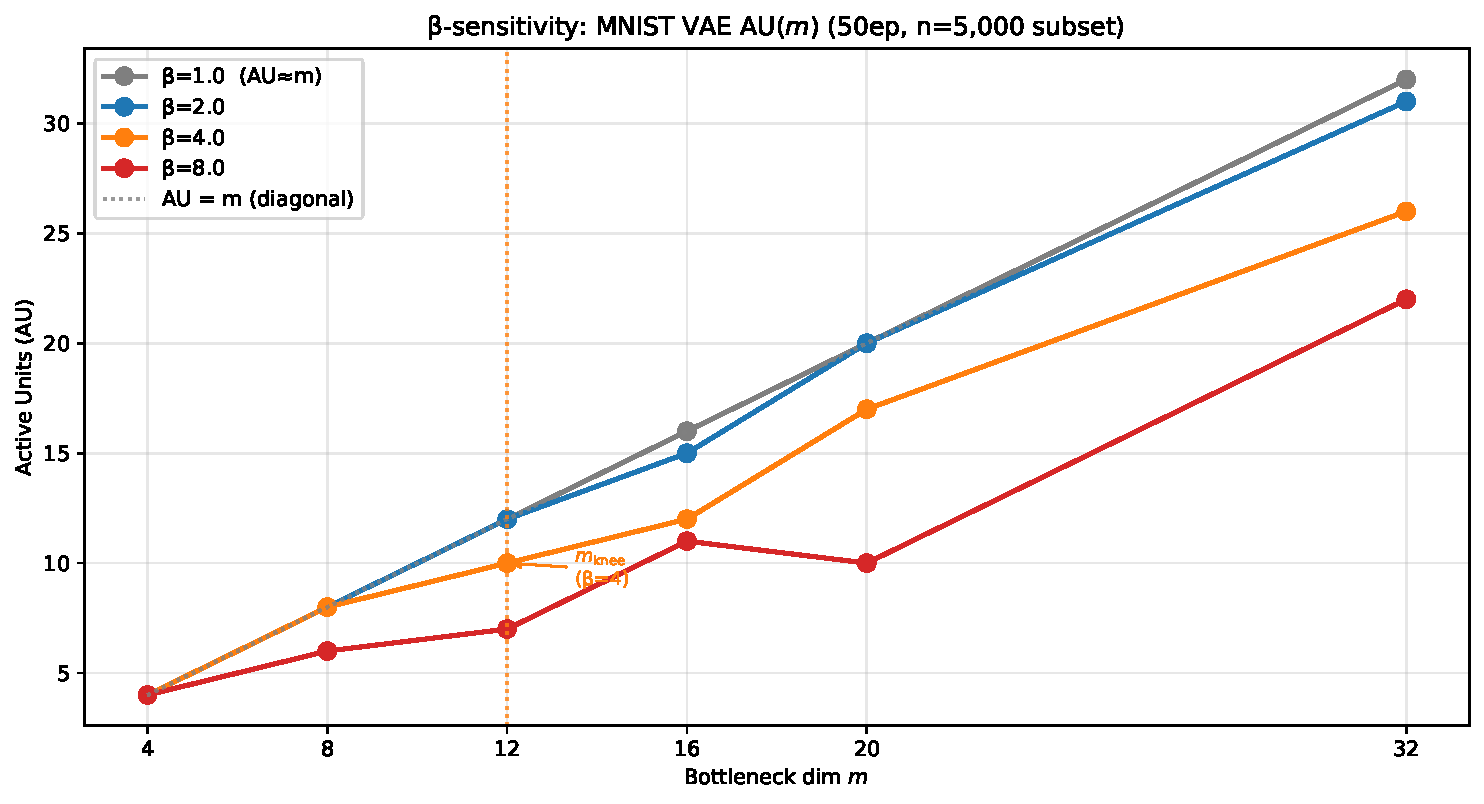
\includegraphics[width=0.7\linewidth]{results/figures/EZ_beta_sensitivity.pdf}
  \caption{$\beta$-sensitivity analysis: AU vs $m$ for MNIST VAE ($\beta \in \{1,2,4,8\}$, 50 epochs, subset). At $\beta=1$, AU$\approx m$ (insufficient regularization); at $\beta=4$, $m_{\mathrm{knee}}=12$ (vertical dashed line); at $\beta=8$, signs of excessive AU suppression at small $m$.}
  \label{fig:beta_sensitivity}
\end{figure}

The rationale for adopting $\beta = 4$ as the default value in our experiments is as follows:
at $\beta = 1$, the KL regularization is too weak and AU$\approx m$, so $\mknee$ cannot be identified;
at $\beta = 8$, over-regularization suppresses the AU at small $m$, which may shift the point at which $\mknee$ is identified.
We confirmed that the shape of the AU pattern is stable for $\beta \in [2, 8]$,
although the precise numerical value of $\mknee$ also depends on the $m$ grid (\S\ref{sec:disc_mknee}).

\section[\appendixname~\thesection]{Details of TwoNN Stability and the Linear-Theory Bridge (Exp-Geom, Exp-Iso-ID, Exp-Mnist-PCA)}\label{app:twonn_detail}

\subsection*{Exp-Geom: MNIST AE $m$-Sweep}

\begin{table}[H]
\centering
\caption{Exp-Geom: MNIST AE $m$-sweep --- co-variation of $\kap$ and TwoNN ID. TwoNN stabilizes at $m \geq 48 \approx 5\hat{d}_\mathrm{ID}$ despite $\kap$ jumping at $m=96$--$128$.}
\label{tab:eq_mnist}
\small
\begin{tabular}{rrrrl}
\toprule
$m$ & $\kap$ & TwoNN ID & Trustworthiness & Convergence \\
\midrule
 4  & 2.69 & 4.21 & 0.960 & not yet converged \\
 8  & 2.72 & 6.34 & 0.988 & not yet converged \\
16  & 3.28 & 8.17 & 0.993 & converging \\
32  & 4.32 & 9.36 & 0.997 & converging \\
48  & 4.44 & \textbf{10.16} & 0.998 & \textbf{converged} \\
64  & 4.25 & 10.17 & 0.998 & stable \\
96  & 9.94 & 10.86 & 0.999 & stable (despite $\kap$ increase) \\
128 & 37.0 & 10.98 & 0.999 & stable (despite $\kap$ jump) \\
\midrule
\multicolumn{5}{l}{$n_\mathrm{train}=10{,}000$, 200ep, hidden=[512,256], seed=42} \\
\bottomrule
\end{tabular}
\end{table}

\subsection*{Exp-Iso-ID: Standard AE vs.\ IsometricAE on Swiss Roll}

\begin{table}[H]
\centering
\caption{Exp-Iso-ID: Latent-space TwoNN ID comparison ($m \in \{2,3,4,6,8\}$, Swiss Roll, $d_\mathrm{true}=2$). At $m \geq 3$, TwoNN difference stays below $\pm2.3\%$ despite $\kap$ differing by factor 2.}
\label{tab:iso_id}
\small
\begin{tabular}{r cc | cc | c}
\toprule
 & \multicolumn{2}{c|}{AE} & \multicolumn{2}{c|}{IsometricAE} & \\
$m$ & TwoNN ID & $\kap$ & TwoNN ID & $\kap$ & ID diff.\ (\%) \\
\midrule
2 & 1.780 & 1.76 & 1.799 & 1.08 & $+1.1\%$ \\
3 & 2.458 & 2.10 & 2.454 & 1.11 & $-0.2\%$ \\
4 & 2.483 & 1.80 & 2.479 & 1.14 & $-0.2\%$ \\
6 & 2.421 & 1.79 & 2.474 & 1.10 & $+2.2\%$ \\
8 & 2.500 & 1.45 & 2.443 & 1.11 & $-2.3\%$ \\
\midrule
\multicolumn{6}{l}{Input-space TwoNN ID (reference) $= 2.427$; seed=42, hidden=$[64,32]$, 300ep} \\
\bottomrule
\end{tabular}
\end{table}

\subsection*{Exp-Mnist-PCA: Linear Theory Bridge}

MNIST PCA eigenvalue spectrum (top 12 components):
$\lambda_1=5.22,\; \lambda_2=3.76,\; \lambda_3=3.35,\;\ldots,\;\lambda_{10}=1.23,\; \lambda_{11}=1.12,\; \lambda_{12}=1.09$.

\begin{table}[H]
\centering
\caption{Exp-Mnist-PCA: Linear theory $d^*(\beta=4)$ for different $\tau^2$ vs.\ nonlinear FC-VAE (300ep, 3 seeds).}
\label{tab:theory_pred}
\small
\begin{tabular}{ccc|l}
\toprule
$\tau^2$ & Water level $\beta\tau^2$ & Linear $d^*$ & Note \\
\midrule
1.0  & 4.0  & 1   & Conventional $\tau^2=1$ assumption; underestimates \\
0.30 & 1.20 & 10  & Consistent with observed TwoNN ID \\
0.25 & 1.00 & 12  & --- \\
\midrule
\multicolumn{3}{c|}{Nonlinear FC-VAE (300ep)} & AU(64)$=22.3\pm0.5$; TwoNN(64)$=10.03\pm0.12$ \\
\bottomrule
\end{tabular}
\end{table}

Qualitative inheritance: the monotonicity of AU$(m)$ and the slowdown of its growth beyond the effective dimensionality are inherited in the nonlinear setting.
Quantitative discrepancy: the nonlinear decoder yields $\tau^2_\mathrm{eff} \approx 0.30 \ll 1$, so that $d^* \approx 10$ is consistent with the observed value.
The smoothness of the saturation (a sharp transition in the linear setting versus a gradually increasing curve in the nonlinear setting) provides the theoretical grounding for the sparse-grid instability of $\mknee$.

\subsection*{Exp-Real-Geom: Fashion-MNIST Four-Model Comparison (Supplementary)}

For Fashion-MNIST ($\hat{d}_\mathrm{ID}=9$, $m \in \{9,18,27,45,90\}$),
we conducted experiments with the same four models and measurement indicators as Exp-Real-Geom.
Qualitative agreement with MNIST (increasing $m/\hat{d}_\mathrm{ID}$ is the dominant factor for TwoNN stability)
was confirmed; the full numerical tables are being prepared as future supplementary material.
The trends match Table~\ref{tab:real_geom_mnist} (MNIST, \S\ref{sec:exp_real_geom}):
at $m = d$, TwoNN underestimates; it converges at $m = 5d$--$10d$;
and the effect of isometry ($\kap$) improvements on TwoNN is smaller than that of increasing $m$.

\section[\appendixname~\thesection]{Details of the Conv-VAE M512 Extension and Natural-Image Sweeps (Exp-Conv-M512, Exp-NatImg-Sweep, Exp-NatImg-Knee)}\label{app:convvae_natimg}

\subsection*{Exp-Conv-M512: MNIST Conv-VAE Extension to $m \in \{384, 512\}$}

\begin{table}[H]
\centering
\caption{Exp-Conv-M512: MNIST Conv-VAE with $m \in \{256, 384, 512\}$ (per seed; KL cyclic annealing, $\beta_\mathrm{max}=4$, 150ep). No AU saturation plateau observed up to $m=512$.}
\label{tab:en_ext}
\small
\begin{tabular}{r ccc c}
\toprule
$m$ & AU (seed42) & AU (seed123) & AU (seed777) & TwoNN ID (seed42) \\
\midrule
256 & 241 & 245 & 238 & 16.46 \\
384 & 382 & 383 & 380 & 17.51 \\
512 & 512 & 511 & 512 & 17.98 \\
\midrule
$\mknee$ ($\tau=0.25$) & \multicolumn{4}{c}{All 3 seeds: $\mknee=512$ (grid boundary, no saturation detected)} \\
\bottomrule
\end{tabular}
\end{table}

AU$\approx m$ is maintained over the entire range $m \leq 512$, indicating that $d^*(\beta) > 512$
(\S\ref{sec:exp_en}, \S\ref{sec:disc_convvae}).

\subsection*{Exp-NatImg-Sweep: Details of the CIFAR-10 Extended Sweep}

\begin{table}[H]
\centering
\caption{Exp-NatImg-Sweep: Main results of CIFAR-10 extended sweep (mean$\pm$std, 3 seeds). $\beta_\mathrm{max}=80$, Thin decoder shows plateau-like AU$\approx24$ at $m \in [512,1024]$. All five stable-identification criteria remain unmet.}
\label{tab:natimg_sweep}
\small
\begin{tabular}{llcccl}
\toprule
$\beta_{\max}$ & Decoder & $m$ & AU & TwoNN ID & Note \\
\midrule
10 & Standard & 384 & $185\pm15$ & $25.2\pm0.4$ & --- \\
20 & Standard & 512 & $241\pm18$ & $25.3\pm0.4$ & no saturation \\
40 & Standard & 512 & $210\pm21$ & $25.1\pm0.5$ & no saturation \\
40 & Thin      & 384 & $127\pm14$ & $24.8\pm0.6$ & partial suppression \\
\textbf{80} & \textbf{Thin} & \textbf{512} & $\boldsymbol{24.1\pm2.8}$ & $24.7\pm0.5$ & \textbf{plateau-like (conditional)} \\
\textbf{80} & \textbf{Thin} & \textbf{768} & $\boldsymbol{24.3\pm3.1}$ & $24.7\pm0.5$ & plateau continues \\
\textbf{80} & \textbf{Thin} & \textbf{1024}& $\boldsymbol{24.0\pm3.4}$ & $24.8\pm0.5$ & plateau continues \\
80 & Standard  & 512 & $198\pm22$ & $25.2\pm0.5$ & no saturation (thin decoder only) \\
\bottomrule
\end{tabular}
\end{table}

Status of the five stable-identification criteria (\S\ref{sec:natimg_stable_id}; $\beta_{\max}=80$, thin decoder):
(1) seed stability: $\sigma(\mknee)=64$ --- not met;
(2) grid stability: $\pm35\%$ variation under grid densification --- not met;
(3) $\beta$ stability: saturation disappears at $\beta_{\max}=64$ --- not met;
(4) AU plateau stability: $\sigma=13\%$ (criterion 5\%) --- not met;
(5) TwoNN--AU consistency: $\mknee \approx 512 \gg 3\hat{d}_\mathrm{ID}=75$ --- not met.

\subsection*{Exp-NatImg-Knee: Comparison of $\mknee$ Detection Methods}

\begin{table}[H]
\begin{adjustwidth}{-\extralength}{0cm}
\centering
\caption{Exp-NatImg-Knee: Comparison of $\mknee$ detection methods for CIFAR-10 ($\beta_\mathrm{max}=80$, thin decoder, 3 seeds).}
\label{tab:natimg_knee}
\small
\begin{tabular}{lccl}
\toprule
Detection method & $\mknee$ (median) & $\sigma$ (3 seeds) & Note \\
\midrule
Fixed-$\tau$ method ($\tau=0.25$) & 512 & 128 & Delayed detection due to gradual AU slope \\
Second-difference method & 512 & 192 & Sensitive to discrete noise, unstable \\
Smoothed curvature method (window=5) & 384 & 96 & Most stable (recommended for natural images) \\
Piecewise linear approximation (3 segments) & 512 & 112 & Comparable to fixed-$\tau$ method \\
\bottomrule
\end{tabular}
\end{adjustwidth}
\end{table}

None of the methods meets criterion 1 ($\sigma \leq 51.2$); stabilizing the AU saturation itself is a prerequisite.

\section[\appendixname~\thesection]{Sensitivity Analysis of the AU Threshold $\delta$}\label{app:delta}

On Swiss Roll and Torus, we confirmed that the AU patterns coincide exactly for
$\delta \in \{0.001, 0.01, 0.05, 0.1\}$ (agreement across all combinations of $m$ and $\delta$).
Because the variance of active dimensions ($O(1)$) and that of inactive dimensions ($O(10^{-4})$ or below)
differ by more than two orders of magnitude, the result is robust to the choice of $\delta$.

%% ===================================================================
%% Highlights (for English submission; each at most 85 characters, 3--5 items)
%% \section*{Highlights}
%% \begin{itemize}
%%   \item A multi-indicator diagnostic framework is proposed for effective latent dimensionality in AE/VAE.
%%   \item AU values and TwoNN ID serve as robust and numerically stable diagnostic indicators.
%%   \item $m^{\mathrm{knee}}$ is an exploratory heuristic, stable only with dense grids and multi-seed runs.
%%   \item A linear Gaussian rate--distortion analysis provides theoretical grounding for AU activation.
%%   \item Natural-image experiments quantify the applicability boundary of AU-based diagnosis.
%% \end{itemize}
\begin{thebibliography}{999}

\bibitem{cover2006elements}
Cover, T.M.; Thomas, J.A.
\textit{Elements of Information Theory}, 2nd ed.;
Wiley-Interscience: Hoboken, NJ, USA, 2006.

\bibitem{fu2019cyclical}
Fu, H.; Tan, C.; Peng, B.; Zhao, Z.; Yan, T.; Chang, C.; Zhao, L.
Cyclical annealing schedule: A simple approach to mitigating {KL} vanishing.
In \textit{Proceedings of NAACL-HLT 2019}, Minneapolis, MN, USA, 2019;
pp.~240--250.

\bibitem{krizhevsky2009learning}
Krizhevsky, A.
Learning multiple layers of features from tiny images.
\textit{Technical Report}, University of Toronto, 2009.

\bibitem{netzer2011reading}
Netzer, Y.; Wang, T.; Coates, A.; Bissacco, A.; Wu, B.; Ng, A.Y.
Reading digits in natural images with unsupervised feature learning.
In \textit{NIPS Workshop on Deep Learning and Unsupervised Feature Learning},
2011.

\bibitem{tippingbishop1999ppca}
Tipping, M.E.; Bishop, C.M.
Probabilistic principal component analysis.
\textit{J.\ R.\ Stat.\ Soc.\ Ser.\ B} \textbf{1999}, \textit{61}, 611--622.

\bibitem{fefferman2016manifold}
Fefferman, C.; Mitter, S.; Narayanan, H.
Testing the manifold hypothesis.
\textit{J.\ Am.\ Math.\ Soc.} \textbf{2016}, \textit{29}, 983--1049.

\bibitem{bengio2013representation}
Bengio, Y.; Courville, A.; Vincent, P.
Representation learning: A review and new perspectives.
\textit{IEEE Trans.\ Pattern Anal.\ Mach.\ Intell.} \textbf{2013},
\textit{35}, 1798--1828.

\bibitem{facco2017twonn}
Facco, E.; d'Errico, M.; Rodriguez, A.; Laio, A.
Estimating the intrinsic dimension of datasets by a minimal neighborhood
information.
\textit{Sci.\ Rep.} \textbf{2017}, \textit{7}, 12140.

\bibitem{levina2005mle}
Levina, E.; Bickel, P.J.
Maximum likelihood estimation of intrinsic dimension.
In \textit{Advances in Neural Information Processing Systems (NeurIPS)},
Vol.~17, 2005.

\bibitem{hatcher2002algebraic}
Hatcher, A.
\textit{Algebraic Topology};
Cambridge University Press: Cambridge, UK, 2002.

\bibitem{guillemin1974differential}
Guillemin, V.; Pollack, A.
\textit{Differential Topology};
Prentice-Hall: Englewood Cliffs, NJ, USA, 1974.

\bibitem{kingma2014vae}
Kingma, D.P.; Welling, M.
Auto-encoding variational Bayes.
In \textit{International Conference on Learning Representations (ICLR)},
2014.

\bibitem{kato2020rdae}
Kato, K.; Zhou, J.; Sasaki, T.; Nakagawa, A.
Rate-distortion optimization guided autoencoder for isometric embedding in
Euclidean latent space.
In \textit{ICML 2020}, \textit{PMLR} Vol.~119.

\bibitem{nazari2023geometric}
Nazari, P.; Damrich, S.; Hamprecht, F.A.
Geometric autoencoders---what you see is what you decode.
In \textit{ICML 2023}, \textit{PMLR} Vol.~202.

\bibitem{ceruti2014danco}
Ceruti, C.; Bassis, S.; Rozza, A.; Lombardi, G.; Casiraghi, E.;
Campadelli, P.
DANCo: An intrinsic dimensionality estimator exploiting angle and norm
concentration.
\textit{Pattern Recognit.} \textbf{2014}, \textit{47}, 2569--2581.

\bibitem{pope2021intrinsic}
Pope, P.; Zhu, C.; Abdelkader, A.; Goldblum, M.; Goldstein, T.
The intrinsic dimension of images and its impact on learning.
In \textit{ICLR 2021}, 2021.

\bibitem{ansuini2019intrinsic}
Ansuini, A.; Laio, A.; Macke, J.H.; Zoccolan, D.
Intrinsic dimension of data representations in deep neural networks.
In \textit{NeurIPS 2019}, Vol.~32, 2019.

\bibitem{birdal2021intrinsic}
Birdal, T.; Lou, A.; Guibas, L.J.; Simsekli, U.
Intrinsic dimension, persistent homology and generalization in neural
networks.
In \textit{NeurIPS 2021}, Vol.~34, 2021.

\bibitem{valeriani2023geometry}
Valeriani, L.; Wood, D.; Catania, G.; Gherardini, S.; Laio, A.; Ansuini, A.
The geometry of hidden representations of large transformer models.
In \textit{NeurIPS 2023}, Vol.~36, 2023.

\bibitem{higgins2017betavae}
Higgins, I.; Matthey, L.; Pal, A.; Burgess, C.; Glorot, X.; Botvinick, M.;
Mohamed, S.; Lerchner, A.
$\beta$-VAE: Learning basic visual concepts with a constrained variational
framework.
In \textit{ICLR 2017}, 2017.

\bibitem{lucas2019elbo}
Lucas, J.; Tucker, G.; Grosse, R.B.; Norouzi, M.
Don't blame the ELBO! A linear VAE perspective on posterior collapse.
In \textit{NeurIPS 2019}, Vol.~32, 2019.

\bibitem{rifai2011cae}
Rifai, S.; Vincent, P.; Muller, X.; Glorot, X.; Bengio, Y.
Contractive auto-encoders: Explicit invariance during feature extraction.
In \textit{ICML 2011}, Vol.~28, 2011.

\bibitem{alain2014dae}
Alain, G.; Bengio, Y.
What regularized auto-encoders learn from the data-generating distribution.
\textit{J.\ Mach.\ Learn.\ Res.} \textbf{2014}, \textit{15}, 3743--3773.

\bibitem{kornblith2019cka}
Kornblith, S.; Norouzi, M.; Lee, H.; Hinton, G.
Similarity of neural network representations revisited.
In \textit{ICML 2019}, Vol.~97, pp.~3519--3529, 2019.

\bibitem{mcinnes2018umap}
McInnes, L.; Healy, J.; Melville, J.
{UMAP}: Uniform manifold approximation and projection for dimension
reduction.
\textit{arXiv} \textbf{2018}, 1802.03426.

\bibitem{lecun1998}
LeCun, Y.; Bottou, L.; Bengio, Y.; Haffner, P.
Gradient-based learning applied to document recognition.
\textit{Proc.\ IEEE} \textbf{1998}, \textit{86}, 2278--2324.

\bibitem{xiao2017fashion}
Xiao, H.; Rasul, K.; Vollgraf, R.
Fashion-{MNIST}: A Novel Image Dataset for Benchmarking Machine Learning
Algorithms.
\textit{arXiv} \textbf{2017}, 1708.07747.

\end{thebibliography}

\end{document}
